% General Numbers: The Number Plane Beyond the Right Angle
% Mostafa Derraz, 2026. Full paper (stage 4 draft, 9 November 2026).
\documentclass[11pt,a4paper]{amsart}

\usepackage[T1]{fontenc}
\usepackage{lmodern}
\usepackage[sc,osf]{mathpazo}
\linespread{1.05}
\usepackage[a4paper,margin=2.8cm,headheight=14pt]{geometry}
\usepackage{microtype}
\usepackage{amsmath,amssymb,amsthm,mathtools}
\usepackage[dvipsnames]{xcolor}
\usepackage{tikz}
\usetikzlibrary{arrows.meta,calc,angles,quotes}
\usepackage{enumitem}
\usepackage{booktabs,longtable,array}
\usepackage[numbers,sort&compress]{natbib}
\usepackage[colorlinks=true,linkcolor=RoyalBlue!70!black,citecolor=RoyalBlue!70!black,urlcolor=RoyalBlue!70!black]{hyperref}
\usepackage[capitalise,nameinlink,noabbrev]{cleveref}
\hypersetup{pdftitle={General Numbers: The Number Plane Beyond the Right Angle},
  pdfauthor={Mostafa Derraz},
  pdfkeywords={General Numbers, General Sinus, Composer Unit, relative plane, oblique frame, complex numbers}}

% ---------- statements (defined after cleveref, so that \Cref names them) ----------
\theoremstyle{plain}
\newtheorem{theorem}{Theorem}[section]
\newtheorem{proposition}[theorem]{Proposition}
\newtheorem{corollary}[theorem]{Corollary}
\newtheorem{lemma}[theorem]{Lemma}
\newtheorem{axiom}[theorem]{Axiom}
\theoremstyle{definition}
\newtheorem{definition}[theorem]{Definition}
\theoremstyle{remark}
\newtheorem{remark}[theorem]{Remark}
\crefname{axiom}{Axiom}{Axioms}

% ---------- notation, as in the book ----------
\newcommand{\pb}{\bar{\phi}}                     % angle of the Composer axis
\newcommand{\Gp}{\mathcal{G}_{\bar{\phi}}}       % Composer Unit
\newcommand{\up}{\vec{u}_{\bar{\phi}}}           % direction of the Composer Unit
\newcommand{\Jp}{\mathcal{J}_{\bar{\phi}}}       % Turning Unit
\newcommand{\GN}{\mathbb{G}}                     % General Numbers
\newcommand{\GNp}{\mathbb{G}_{\bar{\phi}}}       % relative plane
\newcommand{\C}{\mathbb{C}}
\newcommand{\R}{\mathbb{R}}
\renewcommand{\Re}{\operatorname{Re}}            % real part
\DeclareMathOperator{\Com}{Com}                  % Composer part
\DeclareMathOperator{\Sh}{Sh}                    % shadow on the real axis
\DeclareMathOperator{\Ht}{Ht}                    % height above the real axis
\newcommand{\seg}[1]{\lvert #1\rvert}            % length of a segment
\newcommand{\Zb}{\bar{Z}}                        % foot of a projection

\setlist[enumerate]{leftmargin=*,itemsep=2pt}
\raggedbottom

% ---------- the tables of laws in Appendix A ----------
% one row: the name of the law, then the law and its complex case side by side
\newcommand{\gnlaw}[3]{\multicolumn{2}{@{}l@{}}{\small\itshape #1}\\* #2 & #3 \\ \addlinespace[4pt]}
\newenvironment{gnlaws}{%
  \begin{longtable}{@{}>{\small\raggedright\arraybackslash}p{0.62\textwidth}@{\hspace{0.04\textwidth}}>{\small\raggedright\arraybackslash}p{0.32\textwidth}@{}}
  \toprule
  \multicolumn{1}{@{}l}{\textsc{in a relative plane}} & \multicolumn{1}{l@{}}{\textsc{the complex case}} \\
  \midrule
  \endhead
  \bottomrule
  \endlastfoot}
  {\end{longtable}}
% the same, with a wider left column; a line breaks only between two formulas
\newenvironment{gnlawswide}{%
  \begin{longtable}{@{}>{\small\raggedright\arraybackslash\relpenalty=10000 \binoppenalty=10000 }p{0.64\textwidth}@{\hspace{0.03\textwidth}}>{\small\raggedright\arraybackslash}p{0.32\textwidth}@{}}
  \toprule
  \multicolumn{1}{@{}l}{\textsc{in a relative plane}} & \multicolumn{1}{l@{}}{\textsc{the complex case}} \\
  \midrule
  \endhead
  \bottomrule
  \endlastfoot}
  {\end{longtable}}

\begin{document}

\title{General Numbers: The Number Plane Beyond the Right Angle}

\author{Mostafa Derraz}
\address{Independent Scholar, Tangier, Morocco}
\email{m.derraz@proton.me}
\urladdr{https://orcid.org/0000-0002-2307-9298}

\date{9 November 2026}

\subjclass[2020]{Primary 33B10; Secondary 12D99, 51N20, 51M04}
\keywords{General Numbers, General Sinus, Composer Unit, relative plane, oblique frame, two-variable trigonometry, complex numbers, Euler's formula}

\begin{abstract}
Each enlargement of the number system has answered a question that the old numbers could not. The last one in the plane, Wessel's geometric reading of the complex numbers, rests on a right angle: multiplication by $i$ is a quarter turn, and the imaginary axis stands perpendicular to the real one. The General Sinus, a trigonometry of two variables defined on the oblique triangle, has freed sine and cosine from the right angle. This paper frees the frame in which the number plane is read. A General Number is $z = a + b\,\Gp$, where the Composer Unit $\Gp$ is the arrow at the angle $\pb$ to the real axis whose length is fixed, by one axiom, at $\lvert\cos\pb + \sin\pb\rvert$. For each angle the General Numbers form a relative plane, and the complex plane is the relative plane $\pb = \pi/2$. Every true relative plane is the complex plane named in an oblique frame, and we give the isomorphism explicitly. In this frame we derive the Rule of the Square, $\Gp^2 = 2\lvert\Gp\rvert\cos\pb\,\Gp - \lvert\Gp\rvert^2$, the conjugate, division and a Turning Unit $\Jp$ with $\Jp^2 = -1$, and we write Euler's and De Moivre's formulas and the $n$-th roots with the General Sinus. The algebra of each relative plane is that of the elliptic generalized complex numbers; what is new is the frame fixed by the Axiom, its native trigonometry, and the laws of arithmetic written in it. We also extend the product formulas of the General Sinus Transform to any number of factors. All results have been verified symbolically and numerically.
\end{abstract}

\maketitle

%====================================================================
\section{Introduction}\label{sec:intro}
%====================================================================

\subsection{How numbers grow}

Before there were numbers there were notches. A small bone from Border Cave, in the Lebombo Mountains of southern Africa, carries notches cut by a human hand about forty-three thousand years ago \citep{dErrico2012}, and the Ishango bone, some twenty thousand years old, carries marks arranged in groups \citep{BrooksSmith1987}. Whatever they counted, they record the oldest decision in mathematics: that a mark may stand for a thing.

From there the numbers grew, and they grew in a particular way. Each time, a reasonable question was asked that the numbers of the day could not answer, and each time the answer was a new kind of number. What is $3 - 5$? The negative numbers answered it: the red and black counting rods of Han China kept amounts owned apart from amounts owed \citep{Shen1999}, and in 628 Brahmagupta wrote rules for fortunes, debts and zero \citep{Colebrooke1817,Plofker2009}. Which number squares to $2$? The irrational numbers answered it, to the dismay of the Greeks, who found that no fraction would do. Which number squares to $-1$? This answer took longest to accept. In 1545 Cardano divided ten into two parts whose product is forty and found the impossible pair $5 \pm \sqrt{-15}$, whose product is forty all the same \citep{Cardano1545}. In 1572 Bombelli met a case he could not set aside: the cubic $x^3 = 15x + 4$ has the root $4$, yet the formula of the day reached it only through
\[
\sqrt[3]{2 + \sqrt{-121}} + \sqrt[3]{2 - \sqrt{-121}} ,
\]
and only by computing $(2 \pm i)^3 = 2 \pm 11i$ did the impossible numbers deliver the possible answer \citep{Bombelli1572}. Descartes called such numbers imaginary, and did not mean it kindly \citep{Descartes1637}. A modern lecture course puts it plainly: in mathematics we are free to define new objects so long as they contradict nothing we already have, but we cannot choose their consequences \citep{MokhithiShock2020}.

\subsection{The quarter turn}

The consequences of $i$ became visible in 1797, when the surveyor Caspar Wessel presented to the Royal Danish Academy a paper on the analytical representation of direction \citep{Wessel1799}. Describe a direction by a length and an angle, he showed, and the rule \emph{multiply the lengths and add the angles} behaves exactly like a multiplication. Multiplying by $i$ is then a quarter turn about zero, and $i^2 = -1$ says no more than that two quarter turns make a half turn. Argand found the same picture in 1806 \citep{Argand1806}, Gauss gave it his authority and the name \emph{complex} in 1831 \citep{Gauss1831}, and Hamilton made it rigorous in 1837 as an algebra of ordered pairs of real numbers \citep{Hamilton1837}. Euler's formula $e^{i\theta} = \cos\theta + i\sin\theta$ \citep{Euler1748} tied the picture to the trigonometry that astronomers had used since antiquity, whose addition formulas turn out to be nothing but the rule for multiplying numbers of length one.

In 1843 Hamilton tried to do for space what the complex numbers had done for the plane. The rules refused to fit until he let go of a habit that everyone had believed untouchable, that $ab = ba$, and the quaternions followed \citep{Hamilton1844,Kline1972}. So a number system can also grow by giving up one of its habits, as Hamilton found on his walk along the Royal Canal.

\subsection{The silent condition}

This paper lets go of a different habit, and stays in the plane. Two right angles sit, unremarked, at the foundation of the classical picture. The first is in trigonometry: the sine and the cosine are ratios of the sides of a right triangle, and the right angle is a condition of their definition so familiar that it is seldom stated. The second is in the number plane: the imaginary axis stands at a right angle to the real axis, and its unit has length one.

The General Sinus \citep{Derraz2017,Derraz2026GSP} removed the first condition. It defines a sine and a cosine of two variables, a studied angle $\alpha$ and a projection angle $\phi$, as ratios of the sides of an oblique triangle; by the law of sines,
\[
\sin(\alpha, \phi) = \frac{\sin\alpha}{\sin(\alpha + \phi)} , \qquad \cos(\alpha, \phi) = \frac{\sin\phi}{\sin(\alpha + \phi)} ,
\]
and both reduce to the classical functions when $\alpha + \phi = \pi/2$ \citep[Theorem~3.7 and Corollary~3.8]{Derraz2026GSP}. Read on a circle, they are coordinates measured along an axis that leans at the angle $\pb = \alpha + \phi$ to the first \citep[Proposition~4.12]{Derraz2026GSP}. The General Sinus thus gives a freedom of perspective, projection along any angle. This paper carries that freedom into the number plane itself, where it removes the second condition.

Concretely, a \emph{General Number} is
\[
z = a + b\,\Gp , \qquad a, b \in \R ,
\]
where the \emph{Composer Unit} $\Gp$ is the arrow at the angle $\pb$ to the real axis whose length is fixed, by one axiom, at $\lvert\cos\pb + \sin\pb\rvert$, the sum of the shadows of its direction on the two perpendicular axes of the page (\Cref{sec:gnp}). For each angle the General Numbers form a \emph{relative plane} $\GNp$, in which numbers are added part by part and multiplied by Wessel's rule (\Cref{fig:graph-paper}). At $\pb = \pi/2$ the Composer Unit is $i$ and the relative plane is the complex plane. At every other angle the second axis leans, and its unit has a length of its own. The points of a relative plane are the points of the complex plane; what is new is the frame in which they are named (\Cref{cor:bridge}).

\begin{figure}[tb]
\centering
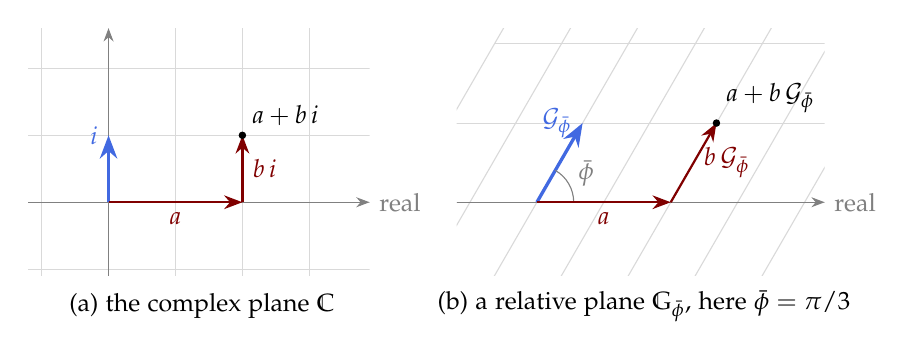
\begin{tikzpicture}[>=Stealth, scale=0.85, every node/.style={font=\small}]
  % ---------- (a) complex plane: square grid ----------
  \begin{scope}
    \clip (-1.2,-1.1) rectangle (3.9,2.6);
    \foreach \a in {-1,...,4} \draw[gray!30] (\a,-1.1) -- (\a,2.6);
    \foreach \b in {-1,...,3} \draw[gray!30] (-1.2,\b) -- (3.9,\b);
  \end{scope}
  \draw[->, gray] (-1.2,0) -- (3.9,0) node[right] {real};
  \draw[->, gray] (0,-1.1) -- (0,2.6);
  \draw[->, very thick, RoyalBlue] (0,0) -- (0,1) node[left] {$i$};
  \draw[->, thick, Maroon] (0,0) -- (2,0) node[below, pos=0.5] {$a$};
  \draw[->, thick, Maroon] (2,0) -- (2,1) node[right, pos=0.5] {$b\,i$};
  \fill (2,1) circle (1.6pt) node[above right] {$a + b\,i$};
  \node at (1.4,-1.55) {(a) the complex plane $\mathbb{C}$};
  % ---------- (b) a relative plane: slanted grid ----------
  \begin{scope}[xshift=6.4cm]
    \pgfmathsetmacro{\gx}{1.366*cos(60)}
    \pgfmathsetmacro{\gy}{1.366*sin(60)}
    \begin{scope}
      \clip (-1.2,-1.1) rectangle (4.3,2.6);
      \foreach \a in {-3,...,5} \draw[gray!30] ($(\a,0)+(-2*\gx,-2*\gy)$) -- ($(\a,0)+(3*\gx,3*\gy)$);
      \foreach \b in {-1,...,2} \draw[gray!30] ($(-2,0)+(\b*\gx,\b*\gy)$) -- ($(5,0)+(\b*\gx,\b*\gy)$);
    \end{scope}
    \draw[->, gray] (-1.2,0) -- (4.3,0) node[right] {real};
    \draw[->, very thick, RoyalBlue] (0,0) -- (\gx,\gy) node[left] {$\mathcal{G}_{\bar{\phi}}$};
    \draw[gray] (0.55,0) arc (0:60:0.55);
    \node[gray] at (30:0.85) {$\bar{\phi}$};
    \draw[->, thick, Maroon] (0,0) -- (2,0) node[below, pos=0.5] {$a$};
    \draw[->, thick, Maroon] (2,0) -- ($(2,0)+(\gx,\gy)$) node[right, pos=0.5] {$b\,\mathcal{G}_{\bar{\phi}}$};
    \fill ($(2,0)+(\gx,\gy)$) circle (1.6pt) node[above right] {$a + b\,\mathcal{G}_{\bar{\phi}}$};
    \node at (1.6,-1.55) {(b) a relative plane $\mathbb{G}_{\bar{\phi}}$, here $\bar{\phi} = \pi/3$};
  \end{scope}
\end{tikzpicture}
\caption{Square and slanted graph paper. (a) In the complex plane, the number $a + bi$ is reached by $a$ steps along the real axis and $b$ steps of length one straight up. (b) In a relative plane, the second family of lines leans at the angle $\pb$, and the number $a + b\,\Gp$ is reached by $a$ steps along the real axis and $b$ steps of the Composer Unit, whose length here is $\cos\frac{\pi}{3} + \sin\frac{\pi}{3} \approx 1.366$. Both pictures use $a = 2$ and $b = 1$.}
\label{fig:graph-paper}
\end{figure}

\subsection{Contributions}

The paper establishes the following. Once a relative plane is identified with $\C$, each proof is short; the interest lies in how the laws read in the leaning frame.
\begin{enumerate}
  \item \emph{The relative planes.} One axiom builds a family of relative planes, one for each angle, which share the real axis and contain the complex plane as the member $\pb = \pi/2$. Every length of the Composer Unit strictly between $1$ and $\sqrt{2}$ belongs to exactly two angles, mirror images of each other about $\pi/4$ (\Cref{sec:gnp}).
  \item \emph{Arithmetic in a leaning frame.} The square of the Composer Unit obeys the Rule of the Square, $\Gp^2 = 2\lvert\Gp\rvert\cos\pb\,\Gp - \lvert\Gp\rvert^2$. The real part of a product, $a_1a_2 - \lvert\Gp\rvert^2 b_1b_2$, depends on the angle only through the length $\lvert\Gp\rvert$. Every true relative plane is a field (\Cref{sec:arith}).
  \item \emph{The conjugate and the skew flip.} The conjugate keeps the mirror image in the real axis but moves the real part to $a + 2b\lvert\Gp\rvert\cos\pb$; the skew flip $a - b\,\Gp$ keeps the real part but not the length (\Cref{sec:arith}).
  \item \emph{The bridge to $\C$.} The Turning Unit $\Jp = -\cot\pb + \Gp/(\lvert\Gp\rvert\sin\pb)$ satisfies $\Jp^2 = -1$, and every General Number is $z = \Sh(z) + \Ht(z)\,\Jp$, its shadow on the real axis plus its height above it. This gives the isomorphism with $\C$ explicitly (\Cref{sec:arith}).
  \item \emph{The laws of the parts.} The Composer part of a product is built from the shadows of the factors, $\Com(z_1z_2) = \Sh(z_1)\Com(z_2) + \Sh(z_2)\Com(z_1)$, and several habits of complex arithmetic fail as soon as the frame leans; \Cref{tab:habits} lists them (\Cref{sec:arith}).
  \item \emph{Turning, powers and roots.} Euler's formula reads $e^{\theta\Jp} = \cos(\theta, \pb - \theta) + \sin(\theta, \pb - \theta)\,\up$, and De Moivre's formula and the $n$-th roots follow, all in the General Sinus. The powers of a number carry two trigonometries at once: the General Sinus in their parts, and the classical sine and cosine in their shadow and height. The powers of the Composer Unit trace a logarithmic spiral, which opens outwards when $\lvert\Gp\rvert > 1$ and winds inwards when $\lvert\Gp\rvert < 1$ (\Cref{sec:turning}).
  \item \emph{The geometry of one magnitude.} Drawn with its parts at right angles, the circle of one magnitude is an ellipse whose axes lie on the diagonals, in the ratio $\tan(\pb/2)$; it is the circle of the elliptic generalized complex numbers, drawn in the chart of the parts. Rings of one magnitude and rays of one angle give each relative plane a polar-like frame (\Cref{sec:magnitude}).
  \item \emph{Products with any number of factors.} The product formulas of the General Sinus Transform, proved in \citep{Derraz2026GSP} for powers of two, hold for any number of factors, as a consequence of the classical product of sines (\Cref{sec:gs}).
\end{enumerate}
Every law has been verified symbolically and numerically, in relative planes at many angles and lengths (\Cref{sec:verify}).

\subsection{What is new and what is not}

A true relative plane is a field with the same points as the complex plane: its arrows are the arrows of the page, its product is Wessel's rule, and the map $z \mapsto \Sh(z) + i\,\Ht(z)$ is an isomorphism of fields onto $\C$ (\Cref{sec:arith}). Every two-dimensional real algebra with a unit is isomorphic to the complex numbers, the dual numbers or the split-complex numbers \citep{KantorSolodovnikov1989}, and each relative plane is of the first kind, so no other outcome was possible. The points are those of $\C$. What is new is the frame in which they are named, the trigonometry native to that frame, and the laws that arithmetic obeys when it is written in it. These laws differ from the familiar ones in ways that matter: in a leaning frame the conjugate does not keep the real part, the Composer part of a product does not follow the real parts of the factors, and the parts of a number can be longer than the number itself.

Two lines of earlier work are close to this one. Oblique coordinates are as old as analytic geometry, and any arrow of the plane can be resolved along two axes that are not perpendicular. Numbers whose unit obeys $i^2 = p + qi$, the generalized complex numbers, have been studied in their own right \citep{HarkinHarkin2004}, and the three kinds of such numbers, complex, dual and double, each carry a geometry of their own \citep{Yaglom1968}. The Rule of the Square is a relation of this kind, with $p = -\lvert\Gp\rvert^2$ and $q = 2\lvert\Gp\rvert\cos\pb$, in the elliptic case $q^2 + 4p < 0$; conversely, every elliptic pair $(p, q)$ is a leaning frame of the page, with the length $\sqrt{-p}$ and the angle $\arccos\bigl(q/(2\sqrt{-p})\bigr)$. The arithmetic of \Cref{sec:arith,sec:turning,sec:magnitude}, which holds for any length of the Composer Unit, is therefore the arithmetic of the elliptic generalized complex numbers, written in a leaning frame, and several of its laws are standard facts about such algebras: the conjugate is the map $\Gp \mapsto q - \Gp$, the squared magnitude is the norm $a^2 + qab - pb^2$, \Cref{thm:division}(1) says that this norm is multiplicative, and the Turning Unit is the element $(\Gp - q/2)/\sqrt{-p - q^2/4}$ by which the elliptic case is reduced to $\C$ \citep{KantorSolodovnikov1989,Yaglom1968}. What this paper adds is the Axiom, which picks one length for each angle; the reading of the frame with the General Sinus, in which the polar form, the turning, Euler's and De Moivre's formulas and the roots are written natively; and the comparison, law by law, of the parts of a number with its shadow and height.

\subsection{A motivation from physics}

The work began with a question from physics, the subject of a forthcoming book by the author. Newton's law of gravitation \citep{Newton1687} and Coulomb's law of electric force \citep{Coulomb1785} have the same shape, a product of two quantities divided by the square of a distance, and a body carries both a mass and a charge. To write the two as one number, one needs a second axis whose unit converts coulombs into kilograms. In SI units the size of that unit is $\sqrt{K/G_{\mathrm{N}}} \approx 1.16043 \times 10^{10}$ kg/C, where $K$ is Coulomb's constant and $G_{\mathrm{N}}$ Newton's, and it is not one. A number plane whose second unit has a length of its own is then a natural setting. The present paper is purely mathematical. Its worked examples use the angle $\pb = 79.86^\circ$, at which the Axiom gives the Composer Unit the length $1.16043$, to five decimals the significand of that constant in SI units. This is the angle used in that application; whether the link survives a change of units is one of the open questions of \Cref{sec:summary}.

\subsection{Organisation of the paper}

\Cref{sec:gs} recalls the General Sinus and extends its products to any number of factors. \Cref{sec:gnp} states the Axiom and builds the relative planes. \Cref{sec:arith} develops the arithmetic of a leaning frame and its bridge to $\C$. \Cref{sec:turning} treats turning, powers and roots, and \Cref{sec:magnitude} the geometry of one magnitude, with the polar-like frame of a relative plane. \Cref{sec:example} works one example through at $79.86^\circ$, \Cref{sec:verify} describes how every result was verified, and \Cref{sec:summary} summarises the results and the questions they leave open. \Cref{app:formulary} collects every law beside its complex case.

%====================================================================
\section{The General Sinus}\label{sec:gs}
%====================================================================

This section recalls the trigonometry of the oblique triangle \citep{Derraz2017,Derraz2026GSP}, cited by the numbering of \citep{Derraz2026GSP}, and adds one result, \Cref{thm:every-n}. Proofs of recalled results are given where they are short.

\subsection{Two angles}\label{subsec:gs-angles}

Let $\alpha$ be an angle with vertex $O$, and let $Z$ be a point on its second side. Classical trigonometry projects $Z$ onto the first side straight down; the foot $\Zb$ makes a right triangle $OZ\Zb$, whose sides give $\cos\alpha$ and $\sin\alpha$. The General Sinus projects $Z$ along a line that makes a chosen angle $\phi$ with $ZO$ (\Cref{fig:projections}). The triangle $OZ\Zb$ is then oblique, with the angle $\alpha$ at $O$, the angle $\phi$ at $Z$ and the angle $\theta = \pi - (\alpha + \phi)$ at $\Zb$. The angle $\alpha$ is the \emph{studied angle} and $\phi$ the \emph{projection angle} \citep[Definition~2.6]{Derraz2026GSP}.

\begin{figure}[tb]
\centering
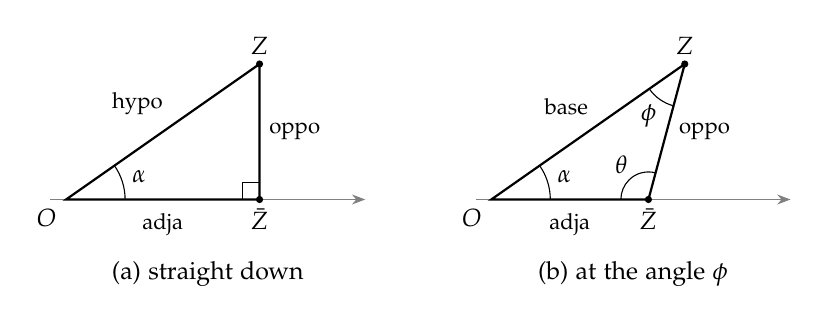
\begin{tikzpicture}[>=Stealth, scale=1.0, every node/.style={font=\small}]
  % ---------- (a) vertical projection ----------
  \begin{scope}
    \coordinate (O) at (0,0);
    \coordinate (X) at (3.6,0);
    \coordinate (Z) at (35:3.0);
    \coordinate (Zb) at ($(O)!(Z)!(X)$);
    \draw[gray, ->] (-0.2,0) -- (3.8,0);
    \draw[thick] (O) -- (Z) -- (Zb) -- cycle;
    \draw ($(Zb)+(-0.22,0)$) -- ++(0,0.22) -- ++(0.22,0);
    \pic [draw, "$\alpha$", angle radius=0.75cm, angle eccentricity=1.3] {angle = X--O--Z};
    \fill (Z) circle (1.3pt) node[above] {$Z$};
    \fill (Zb) circle (1.3pt) node[below] {$\bar{Z}$};
    \node[below left] at (O) {$O$};
    \node[above left, font=\footnotesize] at ($(O)!0.55!(Z)$) {hypo};
    \node[right, font=\footnotesize] at ($(Z)!0.5!(Zb)$) {oppo};
    \node[below, font=\footnotesize] at ($(O)!0.5!(Zb)+(0,-0.05)$) {adja};
    \node at (1.8,-0.95) {(a) straight down};
  \end{scope}
  % ---------- (b) projection at angle phi ----------
  \begin{scope}[xshift=5.4cm]
    \coordinate (O) at (0,0);
    \coordinate (X) at (3.6,0);
    \coordinate (Z) at (35:3.0);
    \coordinate (Zb) at ($(Z)+(255:{3.0*sin(35)/sin(75)})$);
    \draw[gray, ->] (-0.2,0) -- (3.8,0);
    \draw[thick] (O) -- (Z) -- (Zb) -- cycle;
    \pic [draw, "$\alpha$", angle radius=0.75cm, angle eccentricity=1.3] {angle = X--O--Z};
    \pic [draw, "$\phi$", angle radius=0.55cm, angle eccentricity=1.45] {angle = O--Z--Zb};
    \pic [draw, "$\theta$", angle radius=0.35cm, angle eccentricity=1.6] {angle = Z--Zb--O};
    \fill (Z) circle (1.3pt) node[above] {$Z$};
    \fill (Zb) circle (1.3pt) node[below] {$\bar{Z}$};
    \node[below left] at (O) {$O$};
    \node[above left, font=\footnotesize] at ($(O)!0.55!(Z)$) {base};
    \node[right=1pt, font=\footnotesize] at ($(Z)!0.5!(Zb)$) {oppo};
    \node[below, font=\footnotesize] at ($(O)!0.5!(Zb)+(0,-0.05)$) {adja};
    \node at (1.8,-0.95) {(b) at the angle $\phi$};
  \end{scope}
\end{tikzpicture}
\caption{Two ways to project a point $Z$ onto the first side of the angle $\alpha$. (a) Straight down, which gives the right triangle of classical trigonometry. (b) Along a line that makes the projection angle $\phi$ with $ZO$, which gives an oblique triangle with the angles $\alpha$, $\phi$ and $\theta = \pi - (\alpha + \phi)$. The labels hypo, oppo, adja and base abbreviate the hypotenuse, the opposite side, the adjacent side and the base.}
\label{fig:projections}
\end{figure}

\begin{definition}[General trigonometric functions {\citep[Definition~3.6]{Derraz2026GSP}}]\label{def:gs}
The \emph{general sine}, \emph{cosine} and \emph{tangent} are the ratios of the sides of the oblique triangle $OZ\Zb$,
\[
\sin(\alpha, \phi) = \frac{\seg{Z\Zb}}{\seg{OZ}} , \qquad \cos(\alpha, \phi) = \frac{\seg{O\Zb}}{\seg{OZ}} , \qquad \tan(\alpha, \phi) = \frac{\seg{Z\Zb}}{\seg{O\Zb}} ,
\]
where $\seg{PQ}$ is the length of the segment $PQ$, together with their reciprocals $\csc(\alpha, \phi)$, $\sec(\alpha, \phi)$ and $\cot(\alpha, \phi)$.
\end{definition}

\begin{theorem}[Analytic form {\citep[Theorem~3.7]{Derraz2026GSP}}]\label{thm:gs-analytic}
For $\alpha \in \R$ and $\phi \in (0, \pi)$ with $\alpha + \phi \notin \pi\mathbb{Z}$,
\[
\sin(\alpha, \phi) = \frac{\sin\alpha}{\sin(\alpha + \phi)} , \qquad \cos(\alpha, \phi) = \frac{\sin\phi}{\sin(\alpha + \phi)} , \qquad \tan(\alpha, \phi) = \frac{\sin\alpha}{\sin\phi} .
\]
\end{theorem}

\begin{proof}
By the law of sines in $OZ\Zb$, $\seg{Z\Zb}/\sin\alpha = \seg{O\Zb}/\sin\phi = \seg{OZ}/\sin\theta$, and $\sin\theta = \sin(\alpha + \phi)$. The right-hand sides then extend the three functions to all the arguments stated.
\end{proof}

\begin{corollary}[Classical recovery {\citep[Corollary~3.8]{Derraz2026GSP}}]\label{cor:gs-classical}
When $\alpha + \phi = \pi/2$, the triangle is a right triangle and
\[
\sin\bigl(\alpha, \tfrac{\pi}{2} - \alpha\bigr) = \sin\alpha , \qquad \cos\bigl(\alpha, \tfrac{\pi}{2} - \alpha\bigr) = \cos\alpha , \qquad \tan\bigl(\alpha, \tfrac{\pi}{2} - \alpha\bigr) = \tan\alpha .
\]
\end{corollary}

From here on, the formulas of \Cref{thm:gs-analytic} define the general functions for all real $\alpha$ and $\phi$ at which their denominators do not vanish \citep[Proposition~4.1 and Remark~4.2]{Derraz2026GSP}.

\subsection{The composed circle}\label{subsec:gs-circle}

On the unit circle about $O$, draw a second axis, the \emph{Com-axis}, from $O$ at the angle $\pb$ to the $x$-axis; the General Sinus calls $\pb$ the \emph{relative projection angle} \citep[Definitions~2.2 and~2.3]{Derraz2026GSP}. For the point $Z$ of the circle at the studied angle $\alpha$, project $Z$ onto the $x$-axis along the Com-axis. The projection line through $Z$ is parallel to the Com-axis, so it meets $ZO$ at the angle $\phi = \pb - \alpha$ (\Cref{fig:composed-circle}), and the three angles are related by \citep[(2.1)]{Derraz2026GSP}
\[
\pb = \alpha + \phi .
\]

\begin{figure}[tb]
\centering
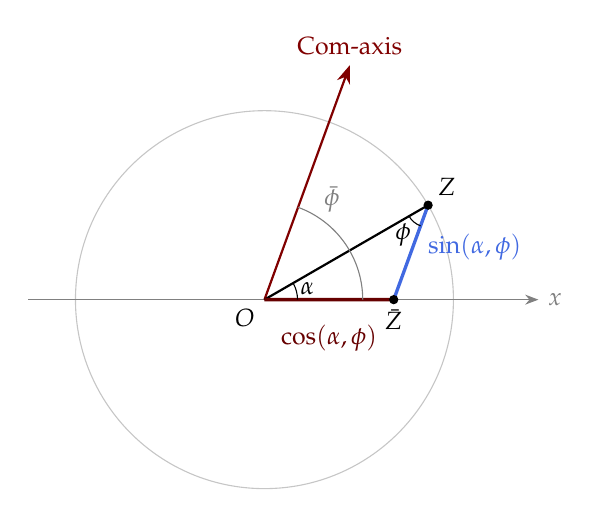
\begin{tikzpicture}[>=Stealth, scale=2.4, every node/.style={font=\small}]
  \def\al{30}
  \def\pbar{70}
  \coordinate (O) at (0,0);
  \coordinate (X) at (1.35,0);
  \coordinate (Z) at (\al:1);
  \coordinate (Zb) at ($(Z)+(\pbar+180:{sin(\al)/sin(\pbar)})$);
  \coordinate (Com) at (\pbar:1.32);
  \draw[gray!45] (O) circle (1);
  \draw[->, gray] (-1.25,0) -- (1.45,0) node[right] {$x$};
  \draw[->, thick, Maroon] (O) -- (Com) node[above] {Com-axis};
  \draw[thick] (O) -- (Z);
  \draw[very thick, RoyalBlue] (Zb) -- (Z);
  \draw[very thick, Maroon!80!black] (O) -- (Zb);
  \pic [draw, "$\alpha$", angle radius=0.42cm, angle eccentricity=1.35] {angle = X--O--Z};
  \draw[gray] (0.52,0) arc (0:\pbar:0.52);
  \node[gray] at (56:0.64) {$\bar{\phi}$};
  \pic [draw, "$\phi$", angle radius=0.28cm, angle eccentricity=1.75] {angle = O--Z--Zb};
  \fill (Z) circle (0.7pt) node[above right] {$Z$};
  \fill (Zb) circle (0.7pt) node[below] {$\bar{Z}$};
  \node[below left] at (O) {$O$};
  \node[below, Maroon!80!black] at ($(O)!0.5!(Zb)+(0,-0.08)$) {$\cos(\alpha,\phi)$};
  \node[right, RoyalBlue] at ($(Zb)!0.55!(Z)+(0.03,0)$) {$\sin(\alpha,\phi)$};
\end{tikzpicture}
\caption{The composed circle. The point $Z$ lies on the unit circle at the studied angle $\alpha$. Projected onto the $x$-axis along the Com-axis, which leans at the angle $\pb = \alpha + \phi$, it has the coordinate $\cos(\alpha, \phi)$ along the $x$-axis and the coordinate $\sin(\alpha, \phi)$ along the Com-axis (\Cref{prop:gs-coordinates}). The picture uses $\alpha = 30^\circ$ and $\pb = 70^\circ$.}
\label{fig:composed-circle}
\end{figure}

\begin{proposition}[Coordinate interpretation {\citep[Proposition~4.12]{Derraz2026GSP}}]\label{prop:gs-coordinates}
Let $0 < \pb < \pi$, let $\up$ be the unit arrow of the Com-axis, and let $Z$ be the point of the unit circle at the angle $\alpha$, with $\phi = \pb - \alpha$. Then
\[
Z = \cos(\alpha, \phi) + \sin(\alpha, \phi)\,\up :
\]
the general cosine is the coordinate of $Z$ along the $x$-axis, and the general sine its coordinate along the Com-axis.
\end{proposition}

\begin{proof}
Write the plane as $\C$, so that $Z = e^{i\alpha}$ and $\up = e^{i\pb}$, and solve $e^{i\alpha} = x + y\,e^{i\pb}$ for real $x$ and $y$. The imaginary parts give $y = \sin\alpha/\sin\pb$, and the real parts give $x = \cos\alpha - y\cos\pb = \sin(\pb - \alpha)/\sin\pb$. With $\pb = \alpha + \phi$ these are $\sin(\alpha, \phi)$ and $\cos(\alpha, \phi)$ (\Cref{thm:gs-analytic}).
\end{proof}

\Cref{prop:gs-coordinates} is the observation on which the rest of this paper is built: the general sine and cosine are the two coordinates of a point in a frame whose second axis leans.

\subsection{Identities}\label{subsec:gs-identities}

All the identities below follow from \Cref{thm:gs-analytic}, on the domains where both sides are defined.

\begin{proposition}[Domains, reciprocity and symmetry {\citep[Propositions~4.1, 4.3, 4.9 and~4.10]{Derraz2026GSP}}]\label{prop:gs-basic}
The general sine and cosine are defined for $\alpha + \phi \notin \pi\mathbb{Z}$, and the general tangent for $\phi \notin \pi\mathbb{Z}$. Moreover,
\begin{enumerate}
  \item \emph{reciprocity:} $\sin(\alpha, \phi) = \cos(\phi, \alpha)$ and $\tan(\alpha, \phi) = \cot(\phi, \alpha)$;
  \item \emph{symmetry:}
  \[
  \sin(-\alpha, -\phi) = \sin(\alpha, \phi) , \qquad \cos(-\alpha, -\phi) = \cos(\alpha, \phi) , \qquad \sin(-\alpha, \phi) = \sin(\alpha, -\phi) ;
  \]
  \item \emph{$\pi$-addition:} for integers $p$ and $q$, $\sin(\alpha + p\pi, \phi + q\pi) = (-1)^q\sin(\alpha, \phi)$ and $\cos(\alpha + p\pi, \phi + q\pi) = (-1)^p\cos(\alpha, \phi)$.
\end{enumerate}
\end{proposition}

\begin{proposition}[The general Pythagoras identity]\label{prop:gs-pythagoras}
For $\alpha + \phi \notin \pi\mathbb{Z}$,
\[
\sin^2(\alpha, \phi) + \cos^2(\alpha, \phi) + 2\sin(\alpha, \phi)\cos(\alpha, \phi)\cos(\alpha + \phi) = 1 .
\]
\end{proposition}

\begin{proof}
Multiplied by $\sin^2(\alpha + \phi)$, the identity reads $\sin^2\alpha + \sin^2\phi + 2\sin\alpha\sin\phi\cos(\alpha + \phi) = \sin^2(\alpha + \phi)$, which follows by expanding $\cos(\alpha + \phi)$ and $\sin(\alpha + \phi)$. In the triangle $OZ\Zb$ with $\seg{OZ} = 1$ it is the law of cosines at $\Zb$.
\end{proof}

At $\alpha + \phi = \pi/2$ the third term vanishes and the identity is $\sin^2\alpha + \cos^2\alpha = 1$.

\begin{theorem}[Addition formulas {\citep[Theorems~5.5 and~5.7]{Derraz2026GSP}}]\label{thm:gs-addition}
On the domains where both sides are defined,
\begin{align*}
\sin(\alpha + \beta, \phi) &= \sin(\alpha, \phi) + \cos(\alpha, \phi)\sin(\beta, \phi + \alpha) , \\
\cos(\alpha + \beta, \phi) &= \cos(\alpha, \phi)\cos(\beta, \phi) + \sin(\alpha, \phi)\sin(\beta, \phi)\cos(\alpha + \beta, \phi) , \\
\sin(\alpha, \phi + \gamma) &= \sin(\alpha, \phi)\sin(\alpha + \phi, \gamma) , \\
\cos(\alpha, \phi + \gamma) &= \cos(\alpha, \phi) + \sin(\alpha, \phi)\cos(\alpha + \phi, \gamma) .
\end{align*}
\end{theorem}

\begin{proof}
The third formula is $\dfrac{\sin\alpha}{\sin(\alpha + \phi + \gamma)} = \dfrac{\sin\alpha}{\sin(\alpha + \phi)} \cdot \dfrac{\sin(\alpha + \phi)}{\sin(\alpha + \phi + \gamma)}$. Cleared of their denominators by \Cref{thm:gs-analytic}, the other three become cases of Ptolemy's identity
\[
\sin(x + y)\sin(y + z) = \sin x\sin z + \sin y\sin(x + y + z) ,
\]
with $(x, y, z) = (\beta, \alpha, \phi)$, $(\alpha, \phi, \beta)$ and $(\gamma, \phi, \alpha)$ in turn. Ptolemy's identity itself follows from $2\sin P\sin Q = \cos(P - Q) - \cos(P + Q)$, since both of its sides equal $\tfrac{1}{2}\bigl[\cos(x - z) - \cos(x + 2y + z)\bigr]$.
\end{proof}

\begin{proposition}[Double angle and derivatives {\citep[Propositions~5.9 and~5.12]{Derraz2026GSP}}]\label{prop:gs-double}
On the domains where both sides are defined,
\begin{gather*}
\sin(2\alpha, \phi) = \sin(\alpha, \phi)\bigl[1 + \cos(2\alpha, \phi)\bigr] , \qquad \cos(2\alpha, \phi) = \cos^2(\alpha, \phi) + \sin^2(\alpha, \phi)\cos(2\alpha, \phi) , \\[3pt]
\frac{\partial}{\partial\alpha}\sin(\alpha, \phi) = \frac{\cos(\alpha, \phi)}{\sin(\alpha + \phi)} , \qquad \frac{\partial}{\partial\phi}\sin(\alpha, \phi) = -\sin(\alpha, \phi)\cot(\alpha + \phi) , \\[3pt]
\frac{\partial}{\partial\alpha}\cos(\alpha, \phi) = -\cos(\alpha, \phi)\cot(\alpha + \phi) , \qquad \frac{\partial}{\partial\phi}\cos(\alpha, \phi) = \frac{\sin(\alpha, \phi)}{\sin(\alpha + \phi)} .
\end{gather*}
\end{proposition}

\begin{proof}
The double-angle formulas are the first two formulas of \Cref{thm:gs-addition} with $\beta = \alpha$, since $\cos(\alpha, \phi)\sin(\alpha, \phi + \alpha) = \sin(\alpha, \phi)\cos(2\alpha, \phi)$. The derivatives follow from \Cref{thm:gs-analytic}.
\end{proof}

\subsection{Products}\label{subsec:gs-products}

The General Sinus Transform writes each general function as a product of scaled copies of itself.

\begin{theorem}[Transformation identities {\citep[Theorem~6.1]{Derraz2026GSP}}]\label{thm:gs-transform}
For every $n \in \mathbb{N}$ and $(x, y)$ in the respective domains,
\begin{gather*}
\sin(x, y) = \prod_{k=0}^{2^n - 1} \sin\Bigl(\frac{x}{2^n} + \pi\frac{k}{2^n}, \frac{y}{2^n}\Bigr) , \qquad \cos(x, y) = \prod_{k=0}^{2^n - 1} \cos\Bigl(\frac{x}{2^n}, \frac{y}{2^n} + \pi\frac{k}{2^n}\Bigr) , \\
\tan(x, y) = \prod_{k=0}^{2^n - 1} \tan\Bigl(\frac{x}{2^n} + \pi\frac{k}{2^n}, \frac{y}{2^n} + \pi\frac{k}{2^n}\Bigr) .
\end{gather*}
\end{theorem}

The proof in \citep{Derraz2026GSP} halves the arguments again and again, which is why the number of factors is a power of two. The products hold for any number of factors, as a short consequence of the classical product of sines.

\begin{corollary}[Products with any number of factors]\label{thm:every-n}
Let $N \geq 1$ be an integer and let $x$ and $y$ be real. If $x + y \notin \pi\mathbb{Z}$, then
\[
\sin(x, y) = \prod_{k=0}^{N-1} \sin\Bigl(\frac{x + \pi k}{N}, \frac{y}{N}\Bigr) , \qquad \cos(x, y) = \prod_{k=0}^{N-1} \cos\Bigl(\frac{x}{N}, \frac{y + \pi k}{N}\Bigr) ,
\]
and if $y \notin \pi\mathbb{Z}$, then
\[
\tan(x, y) = \prod_{k=0}^{N-1} \tan\Bigl(\frac{x + \pi k}{N}, \frac{y + \pi k}{N}\Bigr) .
\]
Every factor lies in the domain of its function. For $N = 2^n$ these are the identities of \Cref{thm:gs-transform}.
\end{corollary}

\begin{proof}
Apply the classical product of sines \citep[\S 1.39]{GradshteynRyzhik2015},
\[
\prod_{k=0}^{N-1} \sin\Bigl(\vartheta + \frac{\pi k}{N}\Bigr) = \frac{\sin(N\vartheta)}{2^{N-1}} ,
\]
with $N\vartheta = x$, with $N\vartheta = y$ and with $N\vartheta = x + y$, and divide:
\begin{gather*}
\frac{\sin x}{\sin(x + y)} = \prod_{k=0}^{N-1} \frac{\sin\bigl((x + \pi k)/N\bigr)}{\sin\bigl((x + \pi k)/N + y/N\bigr)} , \quad \frac{\sin y}{\sin(x + y)} = \prod_{k=0}^{N-1} \frac{\sin\bigl((y + \pi k)/N\bigr)}{\sin\bigl(x/N + (y + \pi k)/N\bigr)} ,\\[2pt]
\frac{\sin x}{\sin y} = \prod_{k=0}^{N-1} \frac{\sin\bigl((x + \pi k)/N\bigr)}{\sin\bigl((y + \pi k)/N\bigr)} .
\end{gather*} By \Cref{thm:gs-analytic} the left sides are $\sin(x, y)$, $\cos(x, y)$ and $\tan(x, y)$, and the factors are the general functions at the stated angles. No denominator vanishes, because the product of the denominators is $\sin(x + y)/2^{N-1} \neq 0$, or $\sin y/2^{N-1} \neq 0$ for the tangent; so every factor lies in its domain.
\end{proof}

As the number of factors grows, the parts $x/N$ and $y/N$ of the arguments become small. Expanding the sine and the cosine of these parts to the second degree, while the shifts $\pi k/N$ are kept exact, turns each factor into a ratio of two polynomials of the second degree, which is the General Sinus Transform proper \citep[Theorem~6.3]{Derraz2026GSP}. It plays for the general functions the part that the Taylor expansion plays for the classical ones, with products in place of sums \citep[Remark~6.4]{Derraz2026GSP}. With \Cref{thm:every-n} the number of factors no longer has to be a power of two.

%====================================================================
\section{The General Number Plane}\label{sec:gnp}
%====================================================================

\subsection{The Axiom}\label{subsec:axiom}

Let $\vec{x}$ and $\vec{y}$ be the two perpendicular unit arrows of the page; $\vec{x}$ points along the real axis.

\begin{axiom}[General Number Plane and Composer Unit]\label{ax:gn}
Let $\pb \in [0, \pi)$ be an angle measured from the real axis. The \emph{Composer Unit} of the angle $\pb$ is the arrow $\Gp = \lvert\Gp\rvert\,\up$ with
\[
\lvert\Gp\rvert = \lvert\cos\pb + \sin\pb\rvert \quad \text{(amplitude)} , \qquad \up = \cos\pb\,\vec{x} + \sin\pb\,\vec{y} \quad \text{(direction)} ,
\]
and the \emph{General Numbers} of the angle $\pb$ are the arrows
\[
z = a + b\,\Gp , \qquad a, b \in \R ,
\]
reached by $a$ steps along the real axis followed by $b$ steps of the Composer Unit.
\end{axiom}

The angle $\pb$ is the angle of the \emph{Composer axis}, the line of $\Gp$, which plays the part of the Com-axis of the composed circle; $\pb$ is its relative projection angle (\Cref{subsec:gs-circle}). The amplitude is the sum of the two shadows of the direction $\up$ on the perpendicular axes of the page, taken without its sign, and it has a second form,
\[
\lvert\Gp\rvert = \lvert\cos\pb + \sin\pb\rvert = \sqrt{2}\,\Bigl\lvert\sin\Bigl(\pb + \frac{\pi}{4}\Bigr)\Bigr\rvert .
\]
It is $1$ at $\pb = 0$ and $\pb = \pi/2$, reaches its largest value $\sqrt{2}$ at $\pi/4$, falls to $0$ at $3\pi/4$ and climbs back towards $1$ as $\pb$ approaches $\pi$ (\Cref{fig:fan}). The real axis keeps its unit of length one, while the Composer axis leans and has a unit of its own: the frame is neither orthogonal nor normalised. Two angles close the plane into a line. At $\pb = 0$ the Composer Unit is $1$, and $1 + 2\,\mathcal{G}_0$ and $2 + \mathcal{G}_0$ are the same number; at $\pb = 3\pi/4$ the Composer Unit has length zero, and every General Number is its own real part.

\begin{definition}[Relative planes, sum and product]\label{def:relative-plane}
For a fixed angle $\pb$, the General Numbers $a + b\,\Gp$ form the \emph{relative plane} $\GNp$, which is \emph{true} when $0 < \pb < \pi$ and $\pb \neq 3\pi/4$. Two numbers of one relative plane are added part by part,
\[
(a_1 + b_1\Gp) + (a_2 + b_2\Gp) = (a_1 + a_2) + (b_1 + b_2)\,\Gp ,
\]
and multiplied by Wessel's rule: their product is the arrow whose length is the product of their lengths and whose angle is the sum of their angles, and a product with $0$ is $0$. The set of all General Numbers, each named in the frame of its own relative plane, is $\GN = \bigcup_{\pb} \GNp$. As sets of arrows, all true relative planes coincide with the page, that is, with $\C$; what distinguishes $\GNp$ is the frame $\{1, \Gp\}$ in which its numbers are named. Numbers are added, multiplied and tested for equality within one relative plane.
\end{definition}

\begin{figure}[tb]
\centering
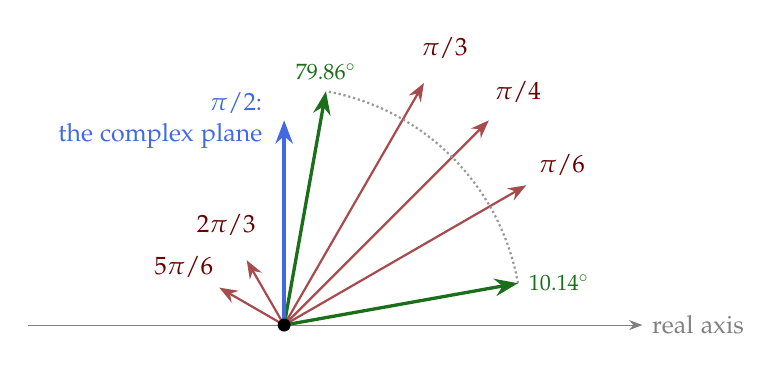
\begin{tikzpicture}[>=Stealth, scale=2.6, every node/.style={font=\small}]
  \draw[->, gray] (-1.25,0) -- (1.75,0) node[right] {real axis};
  \foreach \ang/\len/\lab in {30/1.366/{\pi/6}, 45/1.414/{\pi/4}, 60/1.366/{\pi/3}, 120/0.366/{2\pi/3}, 150/0.366/{5\pi/6}}
  {
    \draw[->, thick, Maroon!70] (0,0) -- (\ang:\len);
    \node[Maroon!80!black] at (\ang:{\len+0.2}) {$\lab$};
  }
  \draw[gray!80, densely dotted, thick] (10.14:1.16043) arc (10.14:79.86:1.16043);
  \draw[->, very thick, ForestGreen!80!black] (0,0) -- (10.14:1.16043) node[right, font=\footnotesize] {$10.14^\circ$};
  \draw[->, very thick, ForestGreen!80!black] (0,0) -- (79.86:1.16043) node[above, font=\footnotesize] {$79.86^\circ$};
  \draw[->, very thick, RoyalBlue] (0,0) -- (90:1) node[left=4pt, align=right, text=RoyalBlue] {$\pi/2$:\\ the complex plane};
  \fill (0,0) circle (0.9pt);
\end{tikzpicture}
\caption{A fan of relative planes. Each arrow is the Composer Unit $\Gp$ of one relative plane, drawn at its angle $\pb$ with the length $\lvert\cos\pb + \sin\pb\rvert$. The upright arrow, of length $1$, is the imaginary unit $i$. The two green arrows have the same length, $1.16043$: they are the two angles of one length (\Cref{thm:two-roots}), and the dotted arc joins them. At $\pb = 3\pi/4$ the length is $0$.}
\label{fig:fan}
\end{figure}

\begin{remark}[On the page]\label{rem:page}
Identify the page with the complex plane, so that $\vec{x}$ is $1$ and $\vec{y}$ is $i$. Then $\up = e^{i\pb}$, the Composer Unit is $\lvert\Gp\rvert\,e^{i\pb}$, and Wessel's rule is the product of complex numbers. We use this identification in the proofs; the statements are about the arrows and their parts in the leaning frame. In a true relative plane the arrows $1$ and $\Gp$ are not parallel, since $\lvert\Gp\rvert \neq 0$ and $\sin\pb \neq 0$. So every arrow of the page is $a + b\,\Gp$ for exactly one pair $(a, b)$, and the product of two numbers of $\GNp$ is again a number of $\GNp$. A true relative plane covers the same points as the complex plane; what changes is the frame in which they are named (\Cref{fig:graph-paper}).
\end{remark}

Except in \Cref{thm:two-roots,thm:square-band} and in the numbers of \Cref{sec:example}, nothing below uses the length that the Axiom gives: every law of \Cref{sec:arith,sec:turning,sec:magnitude} holds for any positive length of the Composer Unit.

\begin{proposition}[Classical recovery]\label{thm:classical-recovery}
At $\pb = \pi/2$ the Composer Unit is the imaginary unit and the relative plane is the complex plane: $\mathcal{G}_{\pi/2} = i$ and $\mathbb{G}_{\pi/2} = \C$.
\end{proposition}

\begin{proof}
At $\pb = \pi/2$ the length is $\lvert 0 + 1\rvert = 1$ and the direction is $\vec{y}$.
\end{proof}

\begin{proposition}[The ladder of number sets]\label{prop:ladder}
The real numbers lie in every relative plane, on the real axis that all of them share, and the complex plane is the relative plane of the right angle:
\[
\mathbb{N} \subset \mathbb{Z} \subset \mathbb{Q} \subset \R \subset \GNp \ \text{ for every } \pb , \qquad \C = \mathbb{G}_{\pi/2} \subset \GN .
\]
\end{proposition}

\begin{proof}
The numbers with $b = 0$ lie on the real axis in every relative plane, and $\mathbb{G}_{\pi/2} = \C$ is \Cref{thm:classical-recovery}.
\end{proof}

The last step of the ladder adds frames, not points: as a set of arrows every true relative plane is $\C$, and $\C$ is the member of the family $\GN$ whose Composer axis stands upright.

\subsection{One length, two angles}\label{subsec:two-roots}

\begin{theorem}[One length, two angles]\label{thm:two-roots}
Let $1 < A < \sqrt{2}$. Exactly two angles $\pb \in [0, \pi)$ give the Composer Unit the length $A$, the \emph{arcsine root} and the \emph{mirror root}
\[
\pb_1 = \arcsin\frac{A}{\sqrt{2}} - \frac{\pi}{4} , \qquad \pb_2 = \frac{\pi}{2} - \pb_1 ,
\]
with $0 < \pb_1 < \pi/4 < \pb_2 < \pi/2$. They are mirror images of each other about the line at the angle $\pi/4$, and
\begin{enumerate}
  \item they exchange their cosine and sine: $\cos\pb_2 = \sin\pb_1$ and $\sin\pb_2 = \cos\pb_1$;
  \item their doubles have the same sine, $\sin 2\pb_1 = \sin 2\pb_2 = A^2 - 1$, so that $\pb_1 = \tfrac{1}{2}\arcsin(A^2 - 1)$;
  \item $\cos 2\pb_1 > 0$ and $\cos 2\pb_2 = -\cos 2\pb_1$.
\end{enumerate}
\end{theorem}

\begin{proof}
For $\pb \in [0, 3\pi/4]$ the length is $\sqrt{2}\sin(\pb + \pi/4)$, and for $\pb \in (3\pi/4, \pi)$ it is less than $1$. Since $A/\sqrt{2} \in (1/\sqrt{2}, 1)$, the equation $\sin(\pb + \pi/4) = A/\sqrt{2}$ has exactly the two solutions $\pb + \pi/4 = \arcsin(A/\sqrt{2})$ and $\pb + \pi/4 = \pi - \arcsin(A/\sqrt{2})$ in $[\pi/4, \pi]$, with $\arcsin(A/\sqrt{2}) \in (\pi/4, \pi/2)$. Statement~(1) is $\cos(\pi/2 - x) = \sin x$. For~(2), $A^2 = (\cos\pb + \sin\pb)^2 = 1 + \sin 2\pb$ at both roots, and $2\pb_1 \in (0, \pi/2)$, where the arcsine gives it back. For~(3), $2\pb_2 = \pi - 2\pb_1$.
\end{proof}

For the length $A = 1.16043$ the two roots are $10.14^\circ$ and $79.86^\circ$; the mirror root is the angle of the worked examples of this paper. The other lengths are found in the same way: the length $\sqrt{2}$ belongs to $\pi/4$ alone, the length $1$ to $0$ and $\pi/2$, a length $0 < A < 1$ to the two angles $3\pi/4 \mp \arcsin(A/\sqrt{2})$, mirror images of each other about $3\pi/4$, and the length $0$ to $3\pi/4$ alone.

\begin{theorem}[Where the square points]\label{thm:square-band}
For $0 \le \pb < \pi$, the square $\Gp^2$ is the arrow of length $\lvert\Gp\rvert^2$ at the angle $2\pb$, with the shadow $\lvert\Gp\rvert^2\cos 2\pb$ on the real axis. The square points backward, its shadow being negative, if and only if
\[
\frac{\pi}{4} < \pb < \frac{3\pi}{4} ,
\]
the \emph{backward band}. For a length $1 < A < \sqrt{2}$, the mirror root lies in the backward band and the arcsine root outside it, and the shadows of the two squares, $\pm A^2\cos 2\pb_1$, have the same size and opposite signs.
\end{theorem}

\begin{proof}
The first statement is Wessel's rule. The length $\lvert\Gp\rvert^2$ is positive except at $3\pi/4$, so the shadow is negative exactly when $2\pb \in (\pi/2, 3\pi/2)$. The rest is \Cref{thm:two-roots}(3).
\end{proof}

The two roots of one length thus give relative planes in which the real part of a product has the same formula (\Cref{prop:product}), while the squares of their Composer Units point in opposite directions.

\subsection{The triangle of a General Number}\label{subsec:triangle}

A General Number $z = a + b\,\Gp \neq 0$ has a \emph{magnitude} $\lvert z\rvert$, the length of its arrow, and an angle $\alpha$ measured from the positive real axis, its studied angle. Its projection angle is $\phi = \pb - \alpha$. When $a > 0$ and $b > 0$, the two legs of its walk, $a$ along the real axis and $b$ steps of the Composer Unit, form with the arrow a triangle with the angles $\alpha$, $\phi$ and $\pi - \pb$; other signs are treated after \Cref{thm:triangle}.

\begin{theorem}[Triangle, magnitude and polar form with two angles]\label{thm:triangle}
Let $z = a + b\,\Gp \neq 0$ lie in a true relative plane, with the angle $\alpha$ and $\phi = \pb - \alpha$. Then
\begin{enumerate}
  \item $\lvert z\rvert^2 = a^2 + 2ab\,\lvert\Gp\rvert\cos\pb + b^2\lvert\Gp\rvert^2$;
  \item $a = \lvert z\rvert\cos(\alpha, \phi)$ and $b\,\lvert\Gp\rvert = \lvert z\rvert\sin(\alpha, \phi)$, that is,
  \[
  z = \lvert z\rvert\,\bigl[\cos(\alpha, \phi) + \sin(\alpha, \phi)\,\up\bigr] , \qquad \alpha + \phi = \pb ;
  \]
  \item if $a \neq 0$ and $1 + \eta\cos\pb \neq 0$, where $\eta = \lvert\Gp\rvert\,b/a$ is the ratio of the two legs, then
  \[
  \alpha = k\pi + \arctan\frac{\eta\sin\pb}{1 + \eta\cos\pb} ,
  \]
  where the integer $k$ is chosen so that $\cos\alpha$ has the sign of $a\,(1 + \eta\cos\pb)$.
\end{enumerate}
\end{theorem}

\begin{proof}
On the page, $z = a + b\,\lvert\Gp\rvert e^{i\pb}$ has the real part $a + b\,\lvert\Gp\rvert\cos\pb$ and the imaginary part $b\,\lvert\Gp\rvert\sin\pb$; the sum of their squares is (1), and their ratio, $\tan\alpha$, gives (3). Statement~(2) is \Cref{prop:gs-coordinates} applied to the unit arrow $z/\lvert z\rvert = e^{i\alpha}$; since $\pb \notin \pi\mathbb{Z}$, the two coordinates in the frame $\{1, \up\}$ are unique.
\end{proof}

At the corner where the real part ends and the Composer part begins, the triangle of $z$ has the angle $\pi - \pb$ when $a$ and $b$ have the same sign, and $\pb$ when their signs differ. When $a$ and $b$ are positive, (1) is the law of cosines and (2) the law of sines in the triangle of $z$. At $\pb = \pi/2$ they are $\lvert z\rvert^2 = a^2 + b^2$ and $z = \lvert z\rvert(\cos\alpha + i\sin\alpha)$, and (3) is the usual argument, $\arctan(b/a)$.

\subsection{The parts and the readings}\label{subsec:parts}

\begin{definition}[Real part, Composer part and Composer coordinate]\label{def:parts}
Let $z = a + b\,\Gp$. The real number $a$ is the \emph{real part} of $z$, written $\Re(z) = a$. The arrow $b\,\Gp$, of length $\lvert b\rvert\,\lvert\Gp\rvert$, is the \emph{Composer part}, written $\Com(z) = b\,\Gp$, and the real number $b$ is the \emph{Composer coordinate}. Every General Number is the sum of its two parts, $z = \Re(z) + \Com(z)$.
\end{definition}

By \Cref{rem:page}, two numbers of one true relative plane are equal if and only if they have the same real part and the same Composer part.

A number with no Composer part is a real number, and the real axis is shared by all the relative planes. A number with no real part, $z = b\,\Gp$, is a \emph{pure Composer number}; in the complex plane these are the imaginary numbers $bi$. In the complex plane the coordinate $b$ and the leg $bi$ have the same length and hardly need two names; here the leg $b\,\Gp$ is $\lvert b\rvert\,\lvert\Gp\rvert$ long, and the names are kept apart.

\begin{definition}[Shadow and height]\label{def:shadow-height}
The \emph{shadow} $\Sh(z)$ of $z$ is the signed length of its perpendicular projection on the real axis, and its \emph{height} $\Ht(z)$ is the signed distance of its tip above the real axis:
\[
\Sh(z) = a + b\,\lvert\Gp\rvert\cos\pb , \qquad \Ht(z) = b\,\lvert\Gp\rvert\sin\pb .
\]
\end{definition}

The parts are read in the leaning frame and the shadow and height in the upright one. In the complex plane the two pairs coincide, $\Sh = \Re$ and $\Ht = \operatorname{Im}$; as soon as the Composer axis leans they differ, and much of \Cref{sec:arith} is about how.

%====================================================================
\section{Arithmetic in a Leaning Frame}\label{sec:arith}
%====================================================================

Throughout this section $z = a + b\,\Gp$ and $w = c + d\,\Gp$ are General Numbers of one true relative plane $\GNp$.

\subsection{The product}\label{subsec:product}

\begin{proposition}[The Rule of the Square]\label{prop:square-rule}
In every true relative plane,
\[
\Gp^2 = 2\,\lvert\Gp\rvert\cos\pb\;\Gp - \lvert\Gp\rvert^2 , \qquad \up^2 = 2\cos\pb\;\up - 1 .
\]
\end{proposition}

\begin{proof}
On the page, $\up = e^{i\pb}$ is a root of $t^2 - 2\cos\pb\,t + 1 = (t - e^{i\pb})(t - e^{-i\pb})$. Multiplying by $\lvert\Gp\rvert^2$ gives the first rule.
\end{proof}

\begin{proposition}[The product]\label{prop:product}
\begin{enumerate}
  \item The product of two General Numbers is
  \[
  zw = \bigl(ac - \lvert\Gp\rvert^2bd\bigr) + \bigl(ad + bc + 2\,\lvert\Gp\rvert\cos\pb\;bd\bigr)\,\Gp .
  \]
  \item Its real part, $\Re(zw) = ac - \lvert\Gp\rvert^2bd$, depends on the angle only through the length $\lvert\Gp\rvert$; it has the same form in the two relative planes of one length (\Cref{thm:two-roots}).
  \item If $\Re(wX) = 0$ for every $w \in \GNp$, then $X = 0$.
\end{enumerate}
\end{proposition}

\begin{proof}
Expand $(a + b\,\Gp)(c + d\,\Gp) = ac + (ad + bc)\,\Gp + bd\,\Gp^2$ and apply \Cref{prop:square-rule}; this proves (1) and (2). For (3), write $X = x + y\,\Gp$. Then $\Re(1 \cdot X) = x$ and $\Re(\Gp X) = -\lvert\Gp\rvert^2y$, so both vanish only if $X = 0$.
\end{proof}

Statement~(3) says that the real parts of products lose nothing: a number is known once the real parts of its products with the numbers of its plane are known.

\begin{proposition}[A relative plane is a field]\label{thm:field}
Every true relative plane $\GNp$, with the sum and product of \Cref{def:relative-plane}, is a field, with zero $0$ and unit $1$.
\end{proposition}

\begin{proof}
By \Cref{rem:page}, $\GNp$ is the set of all arrows of the page, closed under both operations, and they are the operations of $\C$. Every field law therefore holds; the inverse is given explicitly in \Cref{thm:division}.
\end{proof}

\subsection{The conjugate and the skew flip}\label{subsec:conjugate}

\begin{definition}[The conjugate]\label{def:conjugate}
The \emph{conjugate} of $z = a + b\,\Gp$ is $\bar{z} = \bigl(a + 2b\,\lvert\Gp\rvert\cos\pb\bigr) - b\,\Gp$.
\end{definition}

\begin{theorem}[The conjugate]\label{thm:conjugate}
In a true relative plane:
\begin{enumerate}
  \item $\bar{z}$ is the mirror image of $z$ in the real axis;
  \item $\bar{\bar{z}} = z$, $\overline{z + w} = \bar{z} + \bar{w}$ and $\overline{zw} = \bar{z}\,\bar{w}$;
  \item a number and its conjugate add up to twice the shadow, $z + \bar{z} = 2\Sh(z)$;
  \item $z\bar{z} = \lvert z\rvert^2 = a^2 + 2ab\,\lvert\Gp\rvert\cos\pb + b^2\lvert\Gp\rvert^2$, a real number, zero only for $z = 0$;
  \item $\Gp$ and $\overline{\Gp}$ have the sum $2\,\lvert\Gp\rvert\cos\pb$ and the product $\lvert\Gp\rvert^2$, so they are the two roots of $x^2 - 2\,\lvert\Gp\rvert\cos\pb\;x + \lvert\Gp\rvert^2 = 0$, the Rule of the Square.
\end{enumerate}
\end{theorem}

\begin{proof}
On the page, the mirror image of $a + b\,\lvert\Gp\rvert e^{i\pb}$ is $a + b\,\lvert\Gp\rvert e^{-i\pb}$, and $e^{-i\pb} = 2\cos\pb - e^{i\pb}$; this is (1). Statement~(3) is $2a + 2b\,\lvert\Gp\rvert\cos\pb = 2\Sh(z)$. The rest is complex conjugation together with \Cref{thm:triangle}(1).
\end{proof}

\begin{remark}[The skew flip]\label{rem:skew-flip}
The number $a - b\,\Gp$, the \emph{skew flip} of $z$, keeps the real part and reverses the Composer part. It is the reflection of the page in the real axis \emph{along} the Composer axis, and in a leaning frame it is not the conjugate: it changes the length, $\lvert a - b\,\Gp\rvert^2 = \lvert z\rvert^2 - 4ab\,\lvert\Gp\rvert\cos\pb$, and
\[
(a + b\,\Gp)(a - b\,\Gp) = a^2 + b^2\lvert\Gp\rvert^2 - 2b^2\lvert\Gp\rvert\cos\pb\;\Gp
\]
is not real unless $b = 0$. The conjugate keeps the mirror image and the magnitude and gives up the real part; the skew flip keeps the real part and gives up the magnitude. At $\pb = \pi/2$ the two are one.
\end{remark}

\begin{theorem}[Magnitude and division]\label{thm:division}
\begin{enumerate}
  \item The magnitude of a product is the product of the magnitudes, $\lvert zw\rvert = \lvert z\rvert\,\lvert w\rvert$. Written with $zw = s + t\,\Gp$, where $s$ and $t$ are given by \Cref{prop:product}, this is the identity
  \begin{multline*}
  \bigl(a^2 + 2ab\,\lvert\Gp\rvert\cos\pb + b^2\lvert\Gp\rvert^2\bigr)\bigl(c^2 + 2cd\,\lvert\Gp\rvert\cos\pb + d^2\lvert\Gp\rvert^2\bigr) \\
  = s^2 + 2st\,\lvert\Gp\rvert\cos\pb + t^2\lvert\Gp\rvert^2 .
  \end{multline*}
  \item Every $z \neq 0$ has the inverse
  \[
  \frac{1}{z} = \frac{\bar{z}}{\lvert z\rvert^2} = \frac{\bigl(a + 2b\,\lvert\Gp\rvert\cos\pb\bigr) - b\,\Gp}{a^2 + 2ab\,\lvert\Gp\rvert\cos\pb + b^2\lvert\Gp\rvert^2} ,
  \]
  and in particular $1/\Gp = \bigl(2\,\lvert\Gp\rvert\cos\pb - \Gp\bigr)/\lvert\Gp\rvert^2$.
  \item For $w \neq 0$,
  \[
  \frac{z}{w} = \frac{\bigl(ac + 2ad\,\lvert\Gp\rvert\cos\pb + bd\,\lvert\Gp\rvert^2\bigr) + (bc - ad)\,\Gp}{c^2 + 2cd\,\lvert\Gp\rvert\cos\pb + d^2\lvert\Gp\rvert^2} .
  \]
\end{enumerate}
\end{theorem}

\begin{proof}
Lengths multiply by Wessel's rule, and \Cref{thm:triangle}(1) writes each magnitude in its coordinates. The inverse is \Cref{thm:conjugate}(4), and the quotient is $z\bar{w}/\lvert w\rvert^2$ expanded by \Cref{prop:product}.
\end{proof}

At $\pb = \pi/2$ the identity of (1) is the two-square identity $(a^2 + b^2)(c^2 + d^2) = (ac - bd)^2 + (ad + bc)^2$ of Brahmagupta and Fibonacci \citep{Weil1984}; in a leaning frame each sum of two squares becomes a quadratic form with the cross term $2\,\lvert\Gp\rvert\cos\pb$, the norm of the plane, and (1) says that this norm is multiplicative.

\subsection{The Turning Unit and the bridge to the complex plane}\label{subsec:turning-unit}

\begin{definition}[The Turning Unit]\label{def:turning-unit}
The \emph{Turning Unit} of $\GNp$ is
\[
\Jp = \frac{\up - \cos\pb}{\sin\pb} = -\cot\pb + \frac{\Gp}{\lvert\Gp\rvert\sin\pb} .
\]
\end{definition}

\begin{theorem}[The Turning Unit]\label{thm:turning-unit}
In a true relative plane:
\begin{enumerate}
  \item $\Jp$ is the arrow of length $1$ perpendicular to the real axis and pointing upward, the arrow $i$ of the page;
  \item $\Jp^2 = -1$, and $\Jp$ and $-\Jp$ are the only General Numbers whose square is $-1$;
  \item multiplying by $\Jp$ turns every General Number by a right angle and keeps its length;
  \item at $\pb = \pi/2$ the two units are one: $\mathcal{J}_{\pi/2} = \mathcal{G}_{\pi/2} = i$.
\end{enumerate}
\end{theorem}

\begin{proof}
On the page, $(e^{i\pb} - \cos\pb)/\sin\pb = i$. Everything follows from this, since $\GNp$ is a field in which $x^2 = -1$ has at most two roots.
\end{proof}

\begin{proposition}[Shadow and height]\label{prop:shadow-height}
Every General Number is its shadow plus its height times the Turning Unit,
\[
z = \Sh(z) + \Ht(z)\,\Jp , \qquad a = \Sh(z) - \Ht(z)\cot\pb , \quad b = \frac{\Ht(z)}{\lvert\Gp\rvert\sin\pb} .
\]
Moreover $z + \bar{z} = 2\Sh(z)$, $z - \bar{z} = 2\Ht(z)\,\Jp$ and $\lvert z\rvert^2 = \Sh(z)^2 + \Ht(z)^2$.
\end{proposition}

\begin{proof}
On the page, $\Sh(z)$ and $\Ht(z)$ are the real and imaginary parts of $z$, and $\Jp = i$.
\end{proof}

\begin{corollary}[The bridge to $\C$]\label{cor:bridge}
The map $\Phi \colon \GNp \to \C$, $\Phi(z) = \Sh(z) + i\,\Ht(z)$, is an isomorphism of fields. It sends $\Gp$ to $\lvert\Gp\rvert\,e^{i\pb}$ and $\Jp$ to $i$, and it keeps magnitudes and conjugates. Its inverse is
\[
\Phi^{-1}(x + iy) = \bigl(x - y\cot\pb\bigr) + \frac{y}{\lvert\Gp\rvert\sin\pb}\,\Gp .
\]
\end{corollary}

\begin{proof}
$\Phi$ is a bijection by \Cref{prop:shadow-height}, it is additive because $\Sh$ and $\Ht$ are, and it is multiplicative because $z = \Sh(z) + \Ht(z)\,\Jp$ and $\Jp^2 = -1$.
\end{proof}

\Cref{cor:bridge} is the precise sense in which a relative plane holds the points of the complex plane. It also shows what is at stake in the rest of this section: the laws below are the laws of $\C$, read in the leaning frame, and \Cref{tab:habits} shows where a law of the complex plane, copied into the leaning frame with only the names changed, would fail.

\begin{figure}[tb]
\centering
\begin{minipage}[b]{0.42\textwidth}
\centering
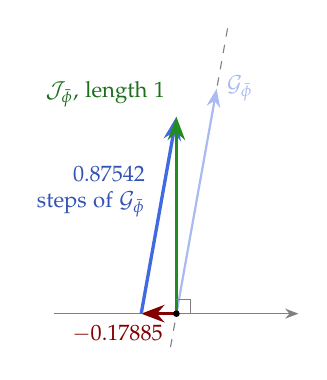
\begin{tikzpicture}[>=Stealth, every node/.style={font=\footnotesize}]
  \def\s{2.5}
  \def\gx{0.20430}\def\gy{1.14231}
  \draw[->, gray] ({-0.62*\s},0) -- ({0.62*\s},0);
  \draw[gray, dashed] ({-0.03*\s},{-0.17*\s}) -- ({0.26*\s},{1.45*\s});
  \draw[->, thick, RoyalBlue!45] (0,0) -- ({\gx*\s},{\gy*\s}) node[right] {$\Gp$};
  \draw[->, very thick, Maroon] (0,0) -- ({-0.17885*\s},0);
  \draw[->, very thick, RoyalBlue] ({-0.17885*\s},0) -- (0,{1.0*\s});
  \draw[->, very thick, ForestGreen] (0,0) -- (0,{1.0*\s});
  \draw[gray] (0.18,0) -- (0.18,0.18) -- (0,0.18);
  \node[ForestGreen!80!black, anchor=south east] at (-0.02,{1.0*\s}) {$\Jp$, length $1$};
  \node[Maroon, below left] at ({-0.02*\s},-0.02) {$-0.17885$};
  \node[RoyalBlue!80!black, anchor=east, align=right] at ({-0.11*\s},{0.62*\s}) {$0.87542$\\ steps of $\Gp$};
  \fill (0,0) circle (1.2pt);
\end{tikzpicture}

\smallskip
{\small (a) the Turning Unit as a walk\par}
\end{minipage}\hfill
\begin{minipage}[b]{0.54\textwidth}
\centering
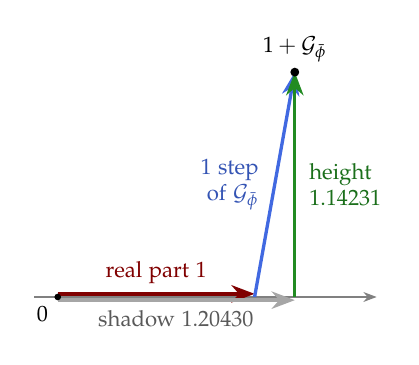
\begin{tikzpicture}[>=Stealth, every node/.style={font=\footnotesize}]
  \def\s{2.5}
  \def\gx{0.20430}\def\gy{1.14231}
  \draw[->, gray] (-0.3,0) -- ({1.62*\s},0);
  \draw[->, very thick, Maroon] (0,0.04) -- ({1*\s},0.04);
  \draw[->, very thick, RoyalBlue] ({1*\s},0) -- ({(1+\gx)*\s},{\gy*\s});
  \draw[->, very thick, gray!70] (0,-0.04) -- ({(1+\gx)*\s},-0.04);
  \draw[->, very thick, ForestGreen] ({(1+\gx)*\s},0) -- ({(1+\gx)*\s},{\gy*\s});
  \fill ({(1+\gx)*\s},{\gy*\s}) circle (1.6pt) node[above] {$1 + \Gp$};
  \node[Maroon, above] at ({0.5*\s},0.05) {real part $1$};
  \node[gray!70!black, below] at ({0.6*\s},-0.05) {shadow $1.20430$};
  \node[RoyalBlue!80!black, anchor=east, align=right] at ({(1+0.5*\gx)*\s-0.08},{0.5*\gy*\s}) {$1$ step\\ of $\Gp$};
  \node[ForestGreen!80!black, anchor=west, align=left] at ({(1+\gx)*\s+0.06},{0.5*\gy*\s}) {height\\ $1.14231$};
  \fill (0,0) circle (1.2pt) node[below left] {$0$};
\end{tikzpicture}

\smallskip
{\small (b) one number, two frames\par}
\end{minipage}
\caption{The Turning Unit at $\pb = 79.86^\circ$, where $\lvert\Gp\rvert = 1.16043$. (a) Its walk goes $-0.17885$ along the real axis and $0.87542$ steps of the Composer Unit, and ends one unit straight above $0$ (\Cref{def:turning-unit}). (b) The number $1 + \Gp$ in the two frames of its plane: in the leaning frame, one step along the real axis and one step of the Composer Unit; in the upright frame, its shadow $1.20430$ and its height $1.14231$ (\Cref{prop:shadow-height}).}
\label{fig:turning-unit}
\end{figure}

\subsection{The laws of the parts}\label{subsec:parts-laws}

\begin{proposition}[From one pair to the other]\label{prop:pairs}
In a true relative plane:
\begin{enumerate}
  \item the parts follow from the readings, and back:
  \begin{align*}
  \Re(z) &= \Sh(z) - \Ht(z)\cot\pb , & \Com(z) &= \frac{\Ht(z)}{\lvert\Gp\rvert\sin\pb}\,\Gp , \\
  \Sh(z) &= \Re(z) + b\,\lvert\Gp\rvert\cos\pb , & \Ht(z) &= b\,\lvert\Gp\rvert\sin\pb ;
  \end{align*}
  \item all four maps are additive and commute with real factors;
  \item the conjugate has the same coordinates on the mirrored unit, $\bar{z} = a + b\,\overline{\Gp}$, and the four are read from $z$ and $\bar{z}$:
  \begin{align*}
  \Re(z) &= \frac{\Gp\bar{z} - \overline{\Gp}z}{\Gp - \overline{\Gp}} , & \Com(z) &= \frac{\Gp\,(z - \bar{z})}{\Gp - \overline{\Gp}} , \\
  \Sh(z) &= \frac{z + \bar{z}}{2} , & \Ht(z)\,\Jp &= \frac{z - \bar{z}}{2} ,
  \end{align*}
  where $\Gp - \overline{\Gp} = 2\,\lvert\Gp\rvert\sin\pb\;\Jp$;
  \item $z$ is a real number exactly when $\bar{z} = z$, and a pure Composer number exactly when $\Gp\bar{z} = \overline{\Gp}z$.
\end{enumerate}
\end{proposition}

\begin{proof}
(1) and (2) follow from \Cref{def:shadow-height} and \Cref{prop:shadow-height}. For (3), conjugation fixes the real numbers $a$ and $b$, so $\bar{z} = a + b\,\overline{\Gp}$; solving the two equations $z = a + b\,\Gp$ and $\bar{z} = a + b\,\overline{\Gp}$ for $a$ and $b$ gives the first line, and the second line is \Cref{prop:shadow-height}. By \Cref{def:turning-unit}, $\Gp - \overline{\Gp} = \lvert\Gp\rvert(\up - \overline{\up}) = 2\,\lvert\Gp\rvert\sin\pb\;\Jp$. Statement~(4) reads (3) with $b = 0$ and with $a = 0$.
\end{proof}

Statement~(3) is the leaning-frame form of $\operatorname{Re} z = (z + \bar{z})/2$: in the complex plane the real part and the shadow coincide, and here it is the shadow that keeps that formula.

\begin{theorem}[The parts of a product]\label{thm:parts-product}
In a true relative plane:
\begin{enumerate}
  \item the parts of a product are
  \[
  \Re(zw) = \Re(z)\Re(w) - \lvert\Gp\rvert^2bd , \qquad \Com(zw) = \Sh(z)\Com(w) + \Sh(w)\Com(z) ;
  \]
  \item its shadow and its height are
  \[
  \Sh(zw) = \Sh(z)\Sh(w) - \Ht(z)\Ht(w) , \qquad \Ht(zw) = \Sh(z)\Ht(w) + \Sh(w)\Ht(z) ;
  \]
  \item for a square, in particular,
  \begin{align*}
  \Re(z^2) &= \Re(z)^2 - \lvert\Gp\rvert^2b^2 , & \Com(z^2) &= 2\Sh(z)\Com(z) , \\
  \Sh(z^2) &= \Sh(z)^2 - \Ht(z)^2 , & \Ht(z^2) &= 2\Sh(z)\Ht(z) .
  \end{align*}
\end{enumerate}
\end{theorem}

\begin{proof}
The real part is \Cref{prop:product}. The Composer coordinate of $zw$ is $ad + bc + 2\,\lvert\Gp\rvert\cos\pb\;bd = (a + b\,\lvert\Gp\rvert\cos\pb)\,d + (c + d\,\lvert\Gp\rvert\cos\pb)\,b = \Sh(z)\,d + \Sh(w)\,b$. Statement (2) is the product rule of $\C$ through \Cref{cor:bridge}, and (3) is (1) with $w = z$.
\end{proof}

The Composer part of a product is thus built from the \emph{shadows} of the factors. The habit $\operatorname{Im}(zw) = \operatorname{Re}(z)\operatorname{Im}(w) + \operatorname{Re}(w)\operatorname{Im}(z)$ of the complex plane, which uses the real parts instead, fails in every leaning frame.

\begin{proposition}[The parts of the conjugate and the inverse]\label{prop:parts-conjugate}
Let $z \neq 0$. Then
\begin{align*}
\Re(\bar{z}) &= 2\Sh(z) - \Re(z) , & \Com(\bar{z}) &= -\Com(z) , & \Sh(\bar{z}) &= \Sh(z) , & \Ht(\bar{z}) &= -\Ht(z) ,
\end{align*}
and
\begin{align*}
\Re\Bigl(\frac{1}{z}\Bigr) &= \frac{2\Sh(z) - \Re(z)}{\lvert z\rvert^2} , & \Com\Bigl(\frac{1}{z}\Bigr) &= -\frac{\Com(z)}{\lvert z\rvert^2} , \\
\Sh\Bigl(\frac{1}{z}\Bigr) &= \frac{\Sh(z)}{\lvert z\rvert^2} , & \Ht\Bigl(\frac{1}{z}\Bigr) &= -\frac{\Ht(z)}{\lvert z\rvert^2} .
\end{align*}
In particular the shadow of $z$ lies halfway between the real parts of $z$ and $\bar{z}$.
\end{proposition}

\begin{proof}
The first line is \Cref{def:conjugate} with \Cref{def:shadow-height}, and the second is the first divided by $\lvert z\rvert^2$ (\Cref{thm:division}).
\end{proof}

\begin{proposition}[The signed area]\label{prop:signed-area}
In a true relative plane,
\begin{align*}
\Com(\bar{z}\,w) &= (ad - bc)\,\Gp , & \Ht(\bar{z}\,w) &= \Sh(z)\Ht(w) - \Ht(z)\Sh(w) , \\
\Re(\bar{z}\,w) &= \Re(\bar{z})\Re(w) + \lvert\Gp\rvert^2bd , & \Sh(\bar{z}\,w) &= \Sh(z)\Sh(w) + \Ht(z)\Ht(w) .
\end{align*}
The height $\Ht(\bar{z}\,w) = (ad - bc)\,\lvert\Gp\rvert\sin\pb$ is the signed area of the parallelogram on the arrows $z$ and $w$, positive when $w$ lies counterclockwise from $z$, and the shadow $\Sh(\bar{z}\,w)$ is $\lvert z\rvert\,\lvert w\rvert$ times the cosine of the angle between them. So $z$ and $w$ lie on one line through $0$ exactly when $ad = bc$, and at a right angle exactly when $\Sh(\bar{z}\,w) = 0$.
\end{proposition}

\begin{proof}
By \Cref{prop:product}, the Composer coordinate of $\bar{z}\,w$ is $(a + 2b\,\lvert\Gp\rvert\cos\pb)\,d - bc - 2\,\lvert\Gp\rvert\cos\pb\;bd = ad - bc$, and its real part is $\Re(\bar{z})\,c + \lvert\Gp\rvert^2bd$. The shadow and the height are \Cref{thm:parts-product}(2) with $\Sh(\bar{z}) = \Sh(z)$ and $\Ht(\bar{z}) = -\Ht(z)$. On the page they are the dot product and the cross product of the arrows $z$ and $w$.
\end{proof}

The Composer coordinate of $\bar{z}\,w$, $ad - bc$, does not depend on the angle at all, and the real part of $zw$ depends on it only through $\lvert\Gp\rvert$; the determinant $ad - bc$ counts cells of the slanted graph paper, each of area $\lvert\Gp\rvert\sin\pb$.

\begin{remark}[Parts longer than the number]\label{rem:longer}
By \Cref{thm:triangle}(2), $\Re(z) = \lvert z\rvert\sin(\pb - \alpha)/\sin\pb$ and $b\,\lvert\Gp\rvert = \lvert z\rvert\sin\alpha/\sin\pb$. Hence
\[
\lvert\Re(z)\rvert \le \frac{\lvert z\rvert}{\sin\pb} , \qquad \lvert\Com(z)\rvert \le \frac{\lvert z\rvert}{\sin\pb} ,
\]
where $\lvert\Com(z)\rvert = \lvert b\rvert\,\lvert\Gp\rvert$ is the length of the Composer part. The real part is longest for a number at a right angle to the Composer axis, and the Composer part for a number at a right angle to the real axis, such as the Turning Unit: its length is $1$, and its Composer part, $\Gp/(\lvert\Gp\rvert\sin\pb)$, is $1/\sin\pb$ long. In a leaning frame a part can thus be longer than its number; at $79.86^\circ$ by at most $1/\sin\pb - 1 \approx 1.6$ per cent. The readings never are: $\lvert\Sh(z)\rvert \le \lvert z\rvert$ and $\lvert\Ht(z)\rvert \le \lvert z\rvert$.
\end{remark}

\begin{table}[tb]
\centering
\small
\renewcommand{\arraystretch}{1.25}
\begin{tabular}{@{}l l@{}}
\toprule
\textbf{a habit of the complex plane} & \textbf{the law in a leaning frame $\GNp$} \\
\midrule
$i^2 = -1$ & $\Gp^2 = 2\,\lvert\Gp\rvert\cos\pb\;\Gp - \lvert\Gp\rvert^2$; it is $\Jp$ that squares to $-1$ \\
$\operatorname{Re}\bar{z} = \operatorname{Re} z$ & $\Re(\bar{z}) = 2\Sh(z) - \Re(z)$ \\
$z + \bar{z} = 2\operatorname{Re} z$ & $z + \bar{z} = 2\Sh(z)$ \\
$z\bar{z} = (\operatorname{Re} z)^2 + (\operatorname{Im} z)^2$ & $z\bar{z} = a^2 + 2ab\,\lvert\Gp\rvert\cos\pb + b^2\lvert\Gp\rvert^2 = \Sh(z)^2 + \Ht(z)^2$ \\
$(a + bi)(a - bi)$ is real & $(a + b\,\Gp)(a - b\,\Gp)$ has the Composer part $-2b^2\lvert\Gp\rvert\cos\pb\;\Gp$ \\
$\operatorname{Im}(zw) = \operatorname{Re} z\operatorname{Im} w + \operatorname{Re} w\operatorname{Im} z$ & $\Com(zw) = \Sh(z)\Com(w) + \Sh(w)\Com(z)$ \\
$\lvert\operatorname{Re} z\rvert \le \lvert z\rvert$ & $\lvert\Re(z)\rvert \le \lvert z\rvert/\sin\pb$, and the bound is reached \\
$(\operatorname{Im} z)\,i$ is the height of $z$ & $\Com(z) = \dfrac{\Ht(z)}{\sin\pb}\,\up$ \\[4pt]
$e^{i\theta} = \cos\theta + i\sin\theta$ & $e^{\theta\Jp} = \cos(\theta, \pb - \theta) + \sin(\theta, \pb - \theta)\,\up$ \\
\bottomrule
\end{tabular}
\caption{Habits of the complex plane and the laws that replace them in a leaning frame, with $z = a + b\,\Gp$. Copied into a relative plane with $i$ replaced by $\Gp$ and the imaginary part by the Composer coordinate, each habit on the left fails as soon as $\cos\pb \neq 0$; each law on the right holds in every true relative plane and becomes the habit on its left at $\pb = \pi/2$.}
\label{tab:habits}
\end{table}

%====================================================================
\section{Turning, Powers and Roots}\label{sec:turning}
%====================================================================

In this section $\theta$ is an angle and, for short,
\[
C_\theta = \cos(\theta, \pb - \theta) = \frac{\sin(\pb - \theta)}{\sin\pb} , \qquad S_\theta = \sin(\theta, \pb - \theta) = \frac{\sin\theta}{\sin\pb} .
\]
By \Cref{thm:triangle}, every number $z \neq 0$ with the angle $\alpha$ is $z = \lvert z\rvert\,(C_\alpha + S_\alpha\,\up)$, and by \Cref{prop:gs-pythagoras}, with $\alpha + \phi = \pb$, the unit numbers obey the general Pythagoras identity $C_\theta^2 + 2\cos\pb\;C_\theta S_\theta + S_\theta^2 = 1$.

\begin{theorem}[Multiplying means turning]\label{thm:turning}
Let $z = \lvert z\rvert\,(C_\alpha + S_\alpha\,\up)$ and $w = \lvert w\rvert\,(C_\beta + S_\beta\,\up)$. Then
\[
zw = \lvert z\rvert\,\lvert w\rvert\,(C_{\alpha + \beta} + S_{\alpha + \beta}\,\up) ,
\]
and, for $w \neq 0$, $z/w$ is the same with $\lvert z\rvert/\lvert w\rvert$ and $\alpha - \beta$. Equivalently, the General Sinus obeys the \emph{addition formulas along the Composer axis},
\[
C_{\alpha + \beta} = C_\alpha C_\beta - S_\alpha S_\beta , \qquad S_{\alpha + \beta} = C_\alpha S_\beta + S_\alpha C_\beta + 2\cos\pb\;S_\alpha S_\beta .
\]
\end{theorem}

\begin{proof}
By Wessel's rule the left side is the arrow of length $\lvert z\rvert\,\lvert w\rvert$ at the angle $\alpha + \beta$, which \Cref{thm:triangle} writes as on the right. Expanding the left side with $\up^2 = 2\cos\pb\;\up - 1$ (\Cref{prop:square-rule}) and comparing parts gives the two formulas.
\end{proof}

Unlike the addition formulas of \Cref{thm:gs-addition}, in which the projection angle stays fixed and the frame moves, these keep the frame fixed: the angle of the Composer axis is $\pb$ throughout. At $\pb = \pi/2$ they are the addition formulas of sine and cosine.

\begin{theorem}[Euler's formula in a relative plane]\label{thm:euler}
For every real $\theta$,
\[
e^{\theta\Jp} = \cos(\theta, \pb - \theta) + \sin(\theta, \pb - \theta)\,\up = C_\theta + S_\theta\,\up .
\]
Consequently every $z \neq 0$ is $z = \lvert z\rvert\,e^{\alpha\Jp}$ and $\bar{z} = \lvert z\rvert\,e^{-\alpha\Jp}$; the two units are exponentials, $\Gp = \lvert\Gp\rvert\,e^{\pb\Jp}$ and $\Jp = e^{(\pi/2)\Jp}$; and $e^{\pi\Jp} + 1 = 0$.
\end{theorem}

\begin{proof}
The exponential series converges in $\GNp$, which is a copy of $\C$ (\Cref{cor:bridge}), and $\Jp^2 = -1$ gives $e^{\theta\Jp} = \cos\theta + \Jp\sin\theta$, the unit arrow at the angle $\theta$. By \Cref{thm:triangle} it is $C_\theta + S_\theta\,\up$. The consequences follow, since $S_{\pb} = 1$ and $C_{\pb} = 0$.
\end{proof}

\begin{remark}[Euler's formula from the derivatives of the General Sinus]\label{rem:euler-native}
The formula can also be reached inside the General Sinus, without the bridge to $\C$. Along the line $\alpha + \phi = \pb$, a change of $\theta$ raises the studied angle and lowers the projection angle by the same amount, so $d/d\theta$ is the partial derivative in the first angle minus the partial derivative in the second. \Cref{prop:gs-double} then gives
\[
\frac{dS_\theta}{d\theta} = \frac{C_\theta}{\sin\pb} + S_\theta\cot\pb , \qquad \frac{dC_\theta}{d\theta} = -C_\theta\cot\pb - \frac{S_\theta}{\sin\pb} .
\]
With $\up^2 = 2\cos\pb\;\up - 1$, these two lines say that the unit number $w(\theta) = C_\theta + S_\theta\,\up$ obeys $dw/d\theta = \Jp\,w$, with $w(0) = 1$, and the only solution of that equation is $e^{\theta\Jp}$. In words, the rate of change of a unit number is its own quarter turn, $\Jp\,w$.
\end{remark}

\begin{theorem}[De Moivre's formula in a relative plane]\label{thm:de-moivre}
For every integer $n$ and every real $\theta$, $(C_\theta + S_\theta\,\up)^n = C_{n\theta} + S_{n\theta}\,\up$.
\end{theorem}

\begin{proof}
Apply \Cref{thm:euler} to $(e^{\theta\Jp})^n = e^{n\theta\Jp}$.
\end{proof}

\begin{corollary}[The powers of the Composer Unit]\label{cor:powers}
For every integer $n$,
\[
\Gp^n = -\lvert\Gp\rvert^n\,\frac{\sin(n - 1)\pb}{\sin\pb} + \lvert\Gp\rvert^{n-1}\,\frac{\sin n\pb}{\sin\pb}\,\Gp ,
\]
and three powers in a row obey the step rule $\Gp^{n+1} = 2\,\lvert\Gp\rvert\cos\pb\;\Gp^n - \lvert\Gp\rvert^2\,\Gp^{n-1}$. For $n \geq 1$ the coefficients $\sin n\pb/\sin\pb$ are the values $U_{n-1}(\cos\pb)$ of the Chebyshev polynomials of the second kind \citep{MasonHandscomb2003}, and for $n = 2$ the formula is the Rule of the Square.
\end{corollary}

\begin{proof}
$\Gp^n = \lvert\Gp\rvert^n(C_{n\pb} + S_{n\pb}\,\up)$ by \Cref{thm:de-moivre} with $\theta = \pb$, and $C_{n\pb} = -\sin(n - 1)\pb/\sin\pb$, $S_{n\pb} = \sin n\pb/\sin\pb$, $\up = \Gp/\lvert\Gp\rvert$. The step rule is the Rule of the Square multiplied by $\Gp^{n-1}$.
\end{proof}

\begin{proposition}[The spiral of powers]\label{prop:spiral}
In a true relative plane, the powers $\Gp^n$, for every integer $n$, are the arrows of length $\lvert\Gp\rvert^n$ at the angles $n\pb$: each multiplication by $\Gp$ turns by $\pb$ and stretches by $\lvert\Gp\rvert$. The powers therefore lie on the logarithmic spiral $\rho = \lvert\Gp\rvert^{\theta/\pb}$, where $\rho$ is the distance from $0$ and $\theta$ the angle on the page, counted continuously, and
\begin{enumerate}
  \item for $0 < \pb < \pi/2$, where $\lvert\Gp\rvert > 1$, the spiral opens outwards;
  \item at $\pb = \pi/2$, where $\lvert\Gp\rvert = 1$, it is the unit circle, and the powers are those of $i$;
  \item for $\pi/2 < \pb < \pi$, where $\lvert\Gp\rvert < 1$, it winds inwards towards $0$;
  \item if $N\pb$ is a whole number of turns, $N\pb = 2\pi k$ with integers $k$ and $N \geq 1$, then $\Gp^N = \lvert\Gp\rvert^N$ is a positive real number.
\end{enumerate}
\end{proposition}

\begin{proof}
By Wessel's rule, $\Gp^n = \lvert\Gp\rvert^n e^{in\pb}$ on the page, which is the point of the spiral at $\theta = n\pb$; for negative $n$ this uses $1/\Gp = \lvert\Gp\rvert^{-1}e^{-i\pb}$. By \Cref{subsec:axiom}, the length $\sqrt{2}\sin(\pb + \pi/4)$ exceeds $1$ exactly for $0 < \pb < \pi/2$, equals $1$ at $\pi/2$, and is below $1$ on $(\pi/2, \pi)$. If $N\pb = 2\pi k$, then $e^{iN\pb} = 1$.
\end{proof}

Raising the Composer Unit to a power is thus a turn, with a change of length at each step (\Cref{fig:spiral}). The two angles of one length share the growth per step but not the turn: at $\pi/3$ and $\pi/6$, the two angles of the length $(1 + \sqrt{3})/2$ (\Cref{thm:two-roots}), the powers grow by the same factor, but they come back to the real axis after six steps in one plane and after twelve in the other. Read in the frame of the plane, the same powers have the parts of \Cref{cor:powers}.

\begin{remark}[The golden ratio at $\pi/5$]\label{rem:golden}
At $\pb = \pi/5$, twice the cosine of the angle is the golden ratio, $2\cos(\pi/5) = \tau = (1 + \sqrt{5})/2$, written $\tau$ here because the letter $\phi$ already names the projection angle. The Rule of the Square then reads $\up^2 = \tau\,\up - 1$, and the coefficients $\sin n\pb/\sin\pb$ of \Cref{cor:powers} are $1$, $\tau$, $\tau$, $1$, $0$ for $n = 1, \dots, 5$, after which they repeat with the opposite sign. So the first powers are
\begin{align*}
\Gp^2 &= -\lvert\Gp\rvert^2 + \tau\,\lvert\Gp\rvert\,\Gp , & \Gp^3 &= -\tau\,\lvert\Gp\rvert^3 + \tau\,\lvert\Gp\rvert^2\,\Gp , \\
\Gp^4 &= -\tau\,\lvert\Gp\rvert^4 + \lvert\Gp\rvert^3\,\Gp , & \Gp^5 &= -\lvert\Gp\rvert^5 .
\end{align*}
After five steps of $36^\circ$ the powers reach the negative real axis, and after ten the positive one, at $\Gp^{10} = \lvert\Gp\rvert^{10} \approx 28.27153$. The length itself, $\lvert\mathcal{G}_{\pi/5}\rvert = \cos 36^\circ + \sin 36^\circ \approx 1.39680$, is not the golden ratio. The golden ratio returns in the General Sinus itself: $\sin(\pi/5, \pi/5) = \cos(\pi/5, \pi/5) = 1/\tau = \tau - 1$, so the general cosecant and secant of $(\pi/5, \pi/5)$ are $\tau$ \citep[Remark~4.8]{Derraz2026GSP}. In the relative plane at $\pb = 2\pi/5$, these two values are $C_{\pi/5}$ and $S_{\pi/5}$, so the unit number on the bisector of the two axes is $e^{(\pi/5)\Jp} = (1 + \up)/\tau$; the sum $1 + \up$, of length $\tau$, is a diagonal of the regular pentagon whose first two sides are $1$ and $\up$.
\end{remark}

\begin{figure}[tb]
\centering
\begin{minipage}[b]{0.32\textwidth}
\centering
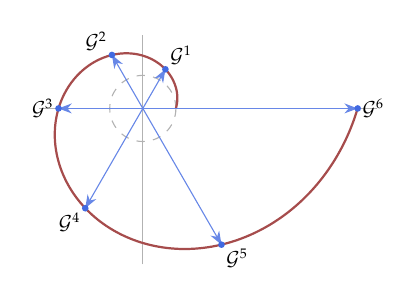
\begin{tikzpicture}[>=Stealth, every node/.style={font=\scriptsize}]
  \draw[gray!60] (-1.321,0) -- (2.979,0);
  \draw[gray!60] (0,-1.98) -- (0,0.929);
  \draw[gray!60, dashed] (0,0) circle (0.42);
  \draw[thick, Maroon!70, smooth, domain=0:360, samples=120, variable=\t] plot (\t:{0.42*1.366025^(\t/60)});
  \draw[->, RoyalBlue!80] (0,0) -- (0.287,0.497);
  \fill[RoyalBlue] (0.287,0.497) circle (1.2pt);
  \node[anchor=south west, inner sep=1.5pt] at (0.287,0.497) {$\mathcal{G}^{1}$};
  \draw[->, RoyalBlue!80] (0,0) -- (-0.392,0.679);
  \fill[RoyalBlue] (-0.392,0.679) circle (1.2pt);
  \node[anchor=south east, inner sep=1.5pt] at (-0.392,0.679) {$\mathcal{G}^{2}$};
  \draw[->, RoyalBlue!80] (0,0) -- (-1.071,0);
  \fill[RoyalBlue] (-1.071,0) circle (1.2pt);
  \node[anchor=east, inner sep=1.5pt] at (-1.071,0) {$\mathcal{G}^{3}$};
  \draw[->, RoyalBlue!80] (0,0) -- (-0.731,-1.267);
  \fill[RoyalBlue] (-0.731,-1.267) circle (1.2pt);
  \node[anchor=north east, inner sep=1.5pt] at (-0.731,-1.267) {$\mathcal{G}^{4}$};
  \draw[->, RoyalBlue!80] (0,0) -- (0.999,-1.73);
  \fill[RoyalBlue] (0.999,-1.73) circle (1.2pt);
  \node[anchor=north west, inner sep=1.5pt] at (0.999,-1.73) {$\mathcal{G}^{5}$};
  \draw[->, RoyalBlue!80] (0,0) -- (2.729,0);
  \fill[RoyalBlue] (2.729,0) circle (1.2pt);
  \node[anchor=west, inner sep=1.5pt] at (2.729,0) {$\mathcal{G}^{6}$};
\end{tikzpicture}

\smallskip
{\footnotesize (a) $\pb = \pi/3$\par}
\end{minipage}\hfill
\begin{minipage}[b]{0.32\textwidth}
\centering
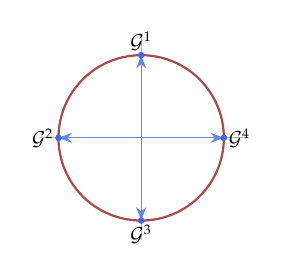
\begin{tikzpicture}[>=Stealth, every node/.style={font=\scriptsize}]
  \draw[gray!60] (-1.3,0) -- (1.3,0);
  \draw[gray!60] (0,-1.3) -- (0,1.3);
  \draw[gray!60, dashed] (0,0) circle (1.05);
  \draw[thick, Maroon!70] (0,0) circle (1.05);
  \draw[->, RoyalBlue!80] (0,0) -- (0,1.05);
  \fill[RoyalBlue] (0,1.05) circle (1.2pt);
  \node[anchor=south, inner sep=1.5pt] at (0,1.05) {$\mathcal{G}^{1}$};
  \draw[->, RoyalBlue!80] (0,0) -- (-1.05,0);
  \fill[RoyalBlue] (-1.05,0) circle (1.2pt);
  \node[anchor=east, inner sep=1.5pt] at (-1.05,0) {$\mathcal{G}^{2}$};
  \draw[->, RoyalBlue!80] (0,0) -- (0,-1.05);
  \fill[RoyalBlue] (0,-1.05) circle (1.2pt);
  \node[anchor=north, inner sep=1.5pt] at (0,-1.05) {$\mathcal{G}^{3}$};
  \draw[->, RoyalBlue!80] (0,0) -- (1.05,0);
  \fill[RoyalBlue] (1.05,0) circle (1.2pt);
  \node[anchor=west, inner sep=1.5pt] at (1.05,0) {$\mathcal{G}^{4}$};
\end{tikzpicture}

\smallskip
{\footnotesize (b) $\pb = \pi/2$\par}
\end{minipage}\hfill
\begin{minipage}[b]{0.32\textwidth}
\centering
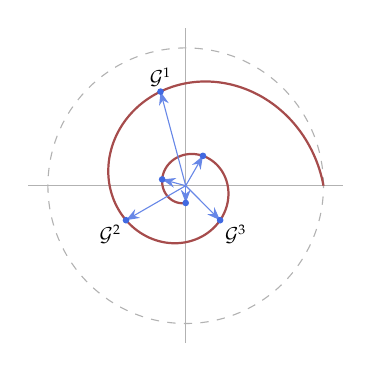
\begin{tikzpicture}[>=Stealth, every node/.style={font=\scriptsize}]
  \draw[gray!60] (-2,0) -- (2,0);
  \draw[gray!60] (0,-2) -- (0,2);
  \draw[gray!60, dashed] (0,0) circle (1.75);
  \draw[thick, Maroon!70, smooth, domain=0:630, samples=210, variable=\t] plot (\t:{1.75*0.707107^(\t/105)});
  \draw[->, RoyalBlue!80] (0,0) -- (-0.32,1.195);
  \fill[RoyalBlue] (-0.32,1.195) circle (1.2pt);
  \node[anchor=south, inner sep=1.5pt] at (-0.32,1.195) {$\mathcal{G}^{1}$};
  \draw[->, RoyalBlue!80] (0,0) -- (-0.758,-0.438);
  \fill[RoyalBlue] (-0.758,-0.438) circle (1.2pt);
  \node[anchor=north east, inner sep=1.5pt] at (-0.758,-0.438) {$\mathcal{G}^{2}$};
  \draw[->, RoyalBlue!80] (0,0) -- (0.437,-0.438);
  \fill[RoyalBlue] (0.437,-0.438) circle (1.2pt);
  \node[anchor=north west, inner sep=1.5pt] at (0.437,-0.438) {$\mathcal{G}^{3}$};
  \draw[->, RoyalBlue!80] (0,0) -- (0.219,0.379);
  \fill[RoyalBlue] (0.219,0.379) circle (1.2pt);
  \draw[->, RoyalBlue!80] (0,0) -- (-0.299,0.08);
  \fill[RoyalBlue] (-0.299,0.08) circle (1.2pt);
  \draw[->, RoyalBlue!80] (0,0) -- (0,-0.219);
  \fill[RoyalBlue] (0,-0.219) circle (1.2pt);
\end{tikzpicture}

\smallskip
{\footnotesize (c) $\pb = 7\pi/12$\par}
\end{minipage}

\bigskip
\begin{minipage}[b]{0.32\textwidth}
\centering
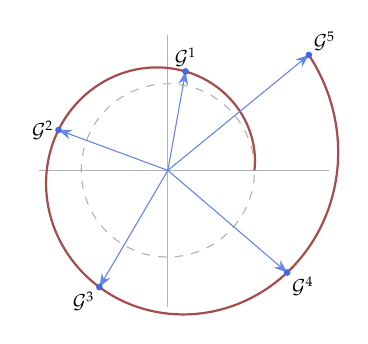
\begin{tikzpicture}[>=Stealth, every node/.style={font=\scriptsize}]
  \draw[gray!60] (-1.639,0) -- (2.041,0);
  \draw[gray!60] (0,-1.732) -- (0,1.716);
  \draw[gray!60, dashed] (0,0) circle (1.1);
  \draw[thick, Maroon!70, smooth, domain=0:399.3, samples=133, variable=\t] plot (\t:{1.1*1.160435^(\t/79.86)});
  \draw[->, RoyalBlue!80] (0,0) -- (0.225,1.257);
  \fill[RoyalBlue] (0.225,1.257) circle (1.2pt);
  \node[anchor=south, inner sep=1.5pt] at (0.225,1.257) {$\mathcal{G}^{1}$};
  \draw[->, RoyalBlue!80] (0,0) -- (-1.389,0.513);
  \fill[RoyalBlue] (-1.389,0.513) circle (1.2pt);
  \node[anchor=east, inner sep=1.5pt] at (-1.389,0.513) {$\mathcal{G}^{2}$};
  \draw[->, RoyalBlue!80] (0,0) -- (-0.87,-1.482);
  \fill[RoyalBlue] (-0.87,-1.482) circle (1.2pt);
  \node[anchor=north east, inner sep=1.5pt] at (-0.87,-1.482) {$\mathcal{G}^{3}$};
  \draw[->, RoyalBlue!80] (0,0) -- (1.515,-1.297);
  \fill[RoyalBlue] (1.515,-1.297) circle (1.2pt);
  \node[anchor=north west, inner sep=1.5pt] at (1.515,-1.297) {$\mathcal{G}^{4}$};
  \draw[->, RoyalBlue!80] (0,0) -- (1.791,1.466);
  \fill[RoyalBlue] (1.791,1.466) circle (1.2pt);
  \node[anchor=south west, inner sep=1.5pt] at (1.791,1.466) {$\mathcal{G}^{5}$};
\end{tikzpicture}

\smallskip
{\footnotesize (d) $\pb = 79.86^\circ$\par}
\end{minipage}\hfill
\begin{minipage}[b]{0.32\textwidth}
\centering
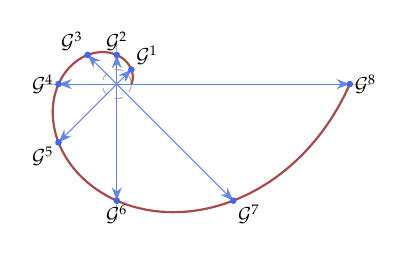
\begin{tikzpicture}[>=Stealth, every node/.style={font=\scriptsize}]
  \draw[gray!60] (-0.99,0) -- (3.21,0);
  \draw[gray!60] (0,-1.73) -- (0,0.62);
  \draw[gray!60, dashed] (0,0) circle (0.185);
  \draw[thick, Maroon!70, smooth, domain=0:360, samples=120, variable=\t] plot (\t:{0.185*1.414214^(\t/45)});
  \draw[->, RoyalBlue!80] (0,0) -- (0.185,0.185);
  \fill[RoyalBlue] (0.185,0.185) circle (1.2pt);
  \node[anchor=south west, inner sep=1.5pt] at (0.185,0.185) {$\mathcal{G}^{1}$};
  \draw[->, RoyalBlue!80] (0,0) -- (0,0.37);
  \fill[RoyalBlue] (0,0.37) circle (1.2pt);
  \node[anchor=south, inner sep=1.5pt] at (0,0.37) {$\mathcal{G}^{2}$};
  \draw[->, RoyalBlue!80] (0,0) -- (-0.37,0.37);
  \fill[RoyalBlue] (-0.37,0.37) circle (1.2pt);
  \node[anchor=south east, inner sep=1.5pt] at (-0.37,0.37) {$\mathcal{G}^{3}$};
  \draw[->, RoyalBlue!80] (0,0) -- (-0.74,0);
  \fill[RoyalBlue] (-0.74,0) circle (1.2pt);
  \node[anchor=east, inner sep=1.5pt] at (-0.74,0) {$\mathcal{G}^{4}$};
  \draw[->, RoyalBlue!80] (0,0) -- (-0.74,-0.74);
  \fill[RoyalBlue] (-0.74,-0.74) circle (1.2pt);
  \node[anchor=north east, inner sep=1.5pt] at (-0.74,-0.74) {$\mathcal{G}^{5}$};
  \draw[->, RoyalBlue!80] (0,0) -- (0,-1.48);
  \fill[RoyalBlue] (0,-1.48) circle (1.2pt);
  \node[anchor=north, inner sep=1.5pt] at (0,-1.48) {$\mathcal{G}^{6}$};
  \draw[->, RoyalBlue!80] (0,0) -- (1.48,-1.48);
  \fill[RoyalBlue] (1.48,-1.48) circle (1.2pt);
  \node[anchor=north west, inner sep=1.5pt] at (1.48,-1.48) {$\mathcal{G}^{7}$};
  \draw[->, RoyalBlue!80] (0,0) -- (2.96,0);
  \fill[RoyalBlue] (2.96,0) circle (1.2pt);
  \node[anchor=west, inner sep=1.5pt] at (2.96,0) {$\mathcal{G}^{8}$};
\end{tikzpicture}

\smallskip
{\footnotesize (e) $\pb = \pi/4$\par}
\end{minipage}\hfill
\begin{minipage}[b]{0.32\textwidth}
\centering
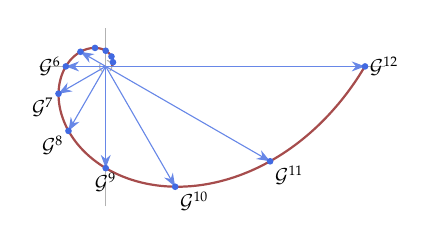
\begin{tikzpicture}[>=Stealth, every node/.style={font=\scriptsize}]
  \draw[gray!60] (-0.85,0) -- (3.543,0);
  \draw[gray!60] (0,-1.778) -- (0,0.485);
  \draw[gray!60, dashed] (0,0) circle (0.078);
  \draw[thick, Maroon!70, smooth, domain=0:360, samples=120, variable=\t] plot (\t:{0.078*1.366025^(\t/30)});
  \fill[RoyalBlue] (0.092,0.053) circle (1.2pt);
  \fill[RoyalBlue] (0.073,0.126) circle (1.2pt);
  \fill[RoyalBlue] (0,0.199) circle (1.2pt);
  \fill[RoyalBlue] (-0.136,0.235) circle (1.2pt);
  \draw[->, RoyalBlue!80] (0,0) -- (-0.321,0.186);
  \fill[RoyalBlue] (-0.321,0.186) circle (1.2pt);
  \draw[->, RoyalBlue!80] (0,0) -- (-0.507,0);
  \fill[RoyalBlue] (-0.507,0) circle (1.2pt);
  \node[anchor=east, inner sep=1.5pt] at (-0.507,0) {$\mathcal{G}^{6}$};
  \draw[->, RoyalBlue!80] (0,0) -- (-0.6,-0.346);
  \fill[RoyalBlue] (-0.6,-0.346) circle (1.2pt);
  \node[anchor=north east, inner sep=1.5pt] at (-0.6,-0.346) {$\mathcal{G}^{7}$};
  \draw[->, RoyalBlue!80] (0,0) -- (-0.473,-0.819);
  \fill[RoyalBlue] (-0.473,-0.819) circle (1.2pt);
  \node[anchor=north east, inner sep=1.5pt] at (-0.473,-0.819) {$\mathcal{G}^{8}$};
  \draw[->, RoyalBlue!80] (0,0) -- (0,-1.292);
  \fill[RoyalBlue] (0,-1.292) circle (1.2pt);
  \node[anchor=north, inner sep=1.5pt] at (0,-1.292) {$\mathcal{G}^{9}$};
  \draw[->, RoyalBlue!80] (0,0) -- (0.882,-1.528);
  \fill[RoyalBlue] (0.882,-1.528) circle (1.2pt);
  \node[anchor=north west, inner sep=1.5pt] at (0.882,-1.528) {$\mathcal{G}^{10}$};
  \draw[->, RoyalBlue!80] (0,0) -- (2.088,-1.205);
  \fill[RoyalBlue] (2.088,-1.205) circle (1.2pt);
  \node[anchor=north west, inner sep=1.5pt] at (2.088,-1.205) {$\mathcal{G}^{11}$};
  \draw[->, RoyalBlue!80] (0,0) -- (3.293,0);
  \fill[RoyalBlue] (3.293,0) circle (1.2pt);
  \node[anchor=west, inner sep=1.5pt] at (3.293,0) {$\mathcal{G}^{12}$};
\end{tikzpicture}

\smallskip
{\footnotesize (f) $\pb = \pi/6$\par}
\end{minipage}
\caption{The spiral of powers of the Composer Unit in six relative planes, drawn on the page (\Cref{prop:spiral}). Each power turns by another $\pb$ and is $\lvert\Gp\rvert$ times longer; the curve is the spiral $\rho = \lvert\Gp\rvert^{\theta/\pb}$, the dashed circle has radius $1$, and each panel has its own scale. (a) $\pb = \pi/3$, $\lvert\Gp\rvert \approx 1.36603$: the powers spiral out and come back to the real axis after six steps, at $\Gp^6 = (26 + 15\sqrt{3})/8 \approx 6.49760$. (b) $\pb = \pi/2$: the powers of $i$ go round the unit circle. (c) $\pb = 7\pi/12 = 105^\circ$, $\lvert\Gp\rvert = \sqrt{2}/2$: the powers spiral in, and their length halves every two steps. (d) $\pb = 79.86^\circ$, the angle of the worked example: each step turns by $79.86^\circ$ and stretches by $16$ per cent; $\Gp^2$ and $\Gp^3$ are the numbers of \Cref{tab:example}. (e) $\pb = \pi/4$, $\lvert\Gp\rvert = \sqrt{2}$: eight steps of $45^\circ$ bring the powers back to the real axis at exactly $\Gp^8 = 16$. (f) $\pb = \pi/6$, the other angle of the length in (a) (\Cref{thm:two-roots}): the same growth per step, but steps of $30^\circ$, so the powers come back only after twelve steps, at $\Gp^{12} \approx 42.21874$; the first five powers are too close to $0$ to be labelled.}
\label{fig:spiral}
\end{figure}

\begin{corollary}[Two trigonometries]\label{cor:two-trig}
Let $z \neq 0$ have the angle $\alpha$. For every integer $n$,
\[
\Re(z^n) = \lvert z\rvert^n C_{n\alpha} , \quad \Com(z^n) = \lvert z\rvert^n S_{n\alpha}\,\up , \qquad \Sh(z^n) = \lvert z\rvert^n\cos n\alpha , \quad \Ht(z^n) = \lvert z\rvert^n\sin n\alpha ,
\]
and for every $z$, $e^{z} = e^{\Sh(z)}\bigl(C_{\Ht(z)} + S_{\Ht(z)}\,\up\bigr)$.
\end{corollary}

\begin{proof}
The first line is \Cref{thm:de-moivre} with \Cref{thm:triangle}(2) and \Cref{prop:shadow-height}. The second follows from $z = \Sh(z) + \Ht(z)\,\Jp$, $e^{w_1 + w_2} = e^{w_1}e^{w_2}$ and \Cref{thm:euler}.
\end{proof}

The powers of a number carry two trigonometries at once: the General Sinus in their parts, read in the leaning frame, and the classical sine and cosine in their shadow and height, read in the upright one.

\begin{theorem}[Roots in a relative plane]\label{thm:roots}
Let $n \geq 1$ and let $z \neq 0$ have the angle $\alpha$. The equation $w^n = z$ has exactly $n$ solutions in $\GNp$,
\[
w_k = \lvert z\rvert^{1/n}\bigl(C_{\theta_k} + S_{\theta_k}\,\up\bigr) , \qquad \theta_k = \frac{\alpha + 2\pi k}{n} , \quad k = 0, 1, \dots, n - 1 .
\]
\end{theorem}

\begin{proof}
By \Cref{thm:de-moivre}, $w_k^n = z$. The $w_k$ are distinct, and a polynomial of degree $n$ has at most $n$ roots in a field.
\end{proof}

\begin{corollary}[The square roots of the Composer Unit]\label{cor:sqrt}
The two square roots of $\Gp$ are
\[
\pm\frac{\sqrt{\lvert\Gp\rvert}}{2\cos(\pb/2)}\,\bigl(1 + \up\bigr) .
\]
The first lies on the ray $\alpha = \pb/2$, which halves the angle between the two axes.
\end{corollary}

\begin{proof}
By the Rule of the Square,
\[
(1 + \up)^2 = 1 + 2\,\up + \up^2 = 2(1 + \cos\pb)\,\up = 4\cos^2(\pb/2)\,\up ,
\]
and on the page $1 + \up = 2\cos(\pb/2)\,e^{i\pb/2}$ with $\cos(\pb/2) > 0$, so $1 + \up$ lies on the ray $\alpha = \pb/2$.
\end{proof}

%====================================================================
\section{The Geometry of One Magnitude}\label{sec:magnitude}
%====================================================================

\subsection{The circle and the ellipse}\label{subsec:circle-ellipse}

\begin{proposition}[The circle of one magnitude]\label{prop:circle}
In a true relative plane, the General Numbers of magnitude $M$ are the points of the circle of radius $M$ about $0$. The line of the Composer axis cuts this circle into two halves: on the half that holds the positive real axis the real parts are positive, and on the other half they are negative.
\end{proposition}

\begin{proof}
By \Cref{thm:triangle}, $\Re(z) = M\sin(\pb - \alpha)/\sin\pb$, which is positive exactly when $\pb - \pi < \alpha < \pb$.
\end{proof}

Drawn in the leaning frame's own chart, with the real part across and the Composer part up at right angles, the same circle is not a circle.

\begin{theorem}[The ellipse of one magnitude]\label{thm:ellipse}
Let $0 < \pb < \pi$ and $M > 0$. Mark each General Number of magnitude $M$ by the pair $(a, B)$ of its real part $a$ and the signed length $B = b\,\lvert\Gp\rvert$ of its Composer part, drawn at right angles, $a$ across and $B$ up. These points form the ellipse
\[
a^2 + B^2 + 2\cos\pb\;aB = M^2 ,
\]
whose axes lie on the diagonals $B = a$ and $B = -a$, with the semi-axes
\[
\frac{M}{\sqrt{1 + \cos\pb}} \ \text{ on } B = a , \qquad \frac{M}{\sqrt{1 - \cos\pb}} \ \text{ on } B = -a .
\]
Their ratio is $\tan(\pb/2)$, the area is $\pi M^2/\sin\pb$, and the eccentricity $e$ is given by $e^2 = 2\lvert\cos\pb\rvert/(1 + \lvert\cos\pb\rvert)$. As the studied angle $\alpha$ makes one turn, the point
\[
a = M\,\frac{\sin(\pb - \alpha)}{\sin\pb} , \qquad B = M\,\frac{\sin\alpha}{\sin\pb}
\]
runs once around the ellipse.
\end{theorem}

\begin{proof}
The equation is \Cref{thm:triangle}(1). Its quadratic form has the matrix $\bigl(\begin{smallmatrix} 1 & \cos\pb \\ \cos\pb & 1 \end{smallmatrix}\bigr)$, with the eigenvalues $1 \pm \cos\pb$ on the eigenvectors $(1, \pm 1)$, both positive for $0 < \pb < \pi$. The semi-axes are $M/\sqrt{1 \pm \cos\pb}$; their ratio is $\sqrt{(1 - \cos\pb)/(1 + \cos\pb)} = \tan(\pb/2)$, the area is $\pi M^2/\sqrt{1 - \cos^2\pb}$, and $e^2$ is one minus the squared ratio of the shorter semi-axis to the longer, $1 - (1 - \lvert\cos\pb\rvert)/(1 + \lvert\cos\pb\rvert)$. The parametric form is \Cref{thm:triangle}(2) with $\phi = \pb - \alpha$. From it, $a + B\cos\pb = M\cos\alpha$ and $B\sin\pb = M\sin\alpha$, so the point $(a, B)$ makes one turn of the ellipse while $(\cos\alpha, \sin\alpha)$ makes one turn of its circle.
\end{proof}

At $\pb = \pi/2$ the ellipse is the circle $a^2 + B^2 = M^2$; as $\pb$ falls towards $0$ it stretches without end along $B = -a$, and at $\pb = 0$ the same equation gives the two parallel lines $a + B = \pm M$. Where the two parts have the same sign the ellipse runs inside the circle of the right angle, and where their signs differ it runs outside, for $\pb < \pi/2$; past the upright the two diagonals trade roles. At $79.86^\circ$ the semi-axes are $0.92212\,M$ on the diagonal $B = a$ and $1.10167\,M$ on $B = -a$, in the ratio $0.83702$ (\Cref{fig:magnitude}).

\begin{figure}[tb]
\centering
\begin{minipage}[b]{0.46\textwidth}
\centering
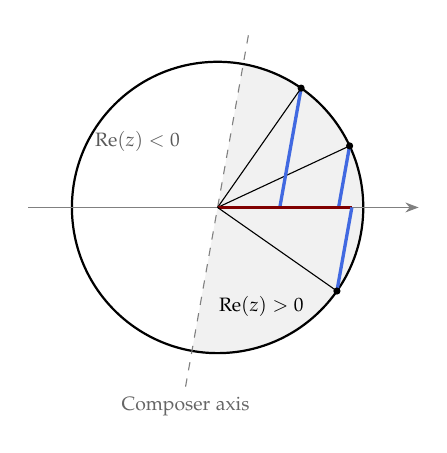
\begin{tikzpicture}[>=Stealth, every node/.style={font=\scriptsize}]
  \def\s{1.85}
  \def\pbar{79.86}
  \fill[gray!11] (\pbar:\s) arc[start angle=\pbar, end angle={\pbar-180}, radius=\s] -- cycle;
  \draw[thick] (0,0) circle (\s);
  \draw[->, gray] ({-1.3*\s},0) -- ({1.38*\s},0);
  \draw[gray, dashed] ({\pbar+180}:{1.25*\s}) -- (\pbar:{1.25*\s});
  \node[gray!80!black, anchor=north] at ({\pbar+180}:{1.25*\s}) {Composer axis};
  \foreach \al in {25,55,-35} {
    \pgfmathsetmacro{\pa}{sin(\pbar-\al)/sin(\pbar)}
    \pgfmathsetmacro{\pB}{sin(\al)/sin(\pbar)}
    \draw[very thick, Maroon] (0,0) -- ({\pa*\s},0);
    \draw[very thick, RoyalBlue] ({\pa*\s},0) -- ++(\pbar:{\pB*\s});
    \draw[thin] (0,0) -- (\al:\s);
    \fill (\al:\s) circle (1.3pt);
  }
  \node[gray!70!black] at ({-0.55*\s},{0.45*\s}) {$\Re(z) < 0$};
  \node at ({0.3*\s},{-0.68*\s}) {$\Re(z) > 0$};
\end{tikzpicture}

\smallskip
{\small (a) on the page: a circle\par}
\end{minipage}\hfill
\begin{minipage}[b]{0.5\textwidth}
\centering
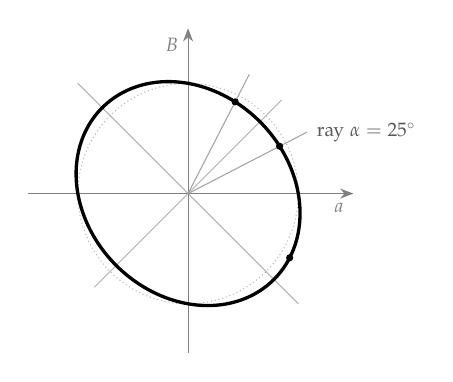
\begin{tikzpicture}[>=Stealth, every node/.style={font=\scriptsize}]
  \def\s{1.4}
  \def\pbar{79.86}
  \draw[gray!55, densely dotted] (0,0) circle (\s);
  \draw[gray!55] ({-0.85*\s},{-0.85*\s}) -- ({0.85*\s},{0.85*\s});
  \draw[gray!55] ({-1.0*\s},{1.0*\s}) -- ({1.0*\s},{-1.0*\s});
  \draw[->, gray] ({-1.45*\s},0) -- ({1.5*\s},0) node[below left] {$a$};
  \draw[->, gray] (0,{-1.45*\s}) -- (0,{1.5*\s}) node[below left] {$B$};
  \draw[very thick, domain=0:360, samples=181, smooth, variable=\t]
    plot ({\s*sin(\pbar-\t)/sin(\pbar)}, {\s*sin(\t)/sin(\pbar)});
  \foreach \al in {25,55} {
    \pgfmathsetmacro{\pa}{sin(\pbar-\al)/sin(\pbar)}
    \pgfmathsetmacro{\pB}{sin(\al)/sin(\pbar)}
    \draw[gray!70] (0,0) -- ({1.3*\pa*\s},{1.3*\pB*\s});
  }
  \pgfmathsetmacro{\qa}{1.3*sin(\pbar-25)/sin(\pbar)}
  \pgfmathsetmacro{\qB}{1.3*sin(25)/sin(\pbar)}
  \node[gray!70!black, anchor=west] at ({\qa*\s},{\qB*\s}) {ray $\alpha = 25^\circ$};
  \foreach \al in {25,55,-35} {
    \pgfmathsetmacro{\pa}{sin(\pbar-\al)/sin(\pbar)}
    \pgfmathsetmacro{\pB}{sin(\al)/sin(\pbar)}
    \fill ({\pa*\s},{\pB*\s}) circle (1.3pt);
  }
\end{tikzpicture}

\smallskip
{\small (b) in the chart: an ellipse\par}
\end{minipage}
\caption{All the General Numbers of one magnitude $M$ at $\pb = 79.86^\circ$. (a) On the page, the tips lie on the circle of radius $M$ (\Cref{prop:circle}); the Composer parts (blue) are parallel to the Composer axis (dashed), whose line cuts the circle into the half of positive real parts (shaded) and the half of negative ones. The three triangles have $\alpha = 25^\circ$, $55^\circ$ and $-35^\circ$. (b) In the chart, the same numbers fill the ellipse $a^2 + B^2 + 2\cos\pb\;aB = M^2$ (\Cref{thm:ellipse}), with the semi-axes $0.92212\,M$ on the diagonal $B = a$ and $1.10167\,M$ on $B = -a$; the dotted circle is the case of a right angle. The three dots are the same numbers in both panels.}
\label{fig:magnitude}
\end{figure}

\subsection{The polar-like frame}\label{subsec:polar-frame}

Polar coordinates name a point of the plane by a distance and an angle, on circles of one distance and rays of one angle. A General Number has a magnitude and an angle too, and the ellipses of \Cref{thm:ellipse} are its circles.

\begin{definition}[Rings and rays]\label{def:rings-rays}
The \emph{chart} of a relative plane is the plane of the pairs $(a, B)$ of \Cref{thm:ellipse}. Its \emph{rings} are the ellipses of one magnitude, and its \emph{rays} are the half-lines from $0$ along which the angle $\alpha$ stays the same. A General Number with the magnitude $M$ and the angle $\alpha$ is the point where its ring and its ray cross.
\end{definition}

Rings and rays are the polar coordinates of the leaning frame. Only at $\pb = \pi/2$ are the rings circles and the rays evenly spread: the chart is then the polar frame of the complex plane. \Cref{fig:polar-frame} draws the frame of two relative planes, in the manner of polar graph paper, and \Cref{rem:frame-readings} says how to read it.

\begin{figure}[tb]
\centering
\begin{minipage}[b]{0.49\textwidth}
\centering
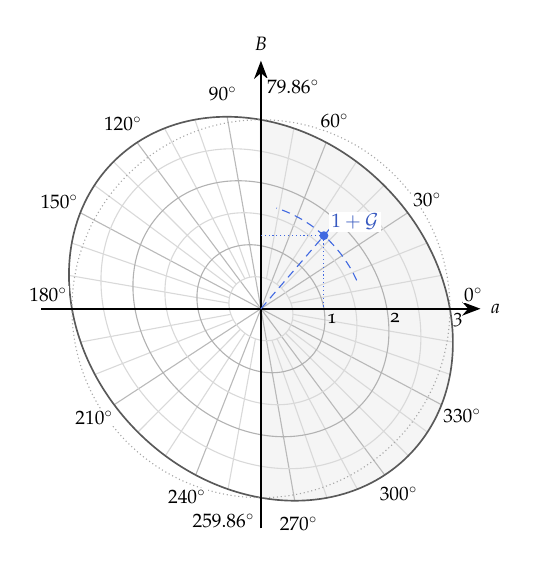
\begin{tikzpicture}[>=Stealth, every node/.style={font=\scriptsize}]
  \begin{scope}\clip (0,-2.788) rectangle (2.788,2.788); \fill[gray!8, rotate=45] (0,0) ellipse ({2.213} and {2.644}); \end{scope}
  \draw[gray!55] (0,0) -- (2.4,0);
  \draw[gray!30] (0.382,0.071) -- (2.289,0.423);
  \draw[gray!30] (0.351,0.139) -- (2.108,0.834);
  \draw[gray!55] (0,0) -- (1.864,1.219);
  \draw[gray!30] (0.26,0.261) -- (1.563,1.567);
  \draw[gray!30] (0.202,0.311) -- (1.214,1.868);
  \draw[gray!55] (0,0) -- (0.828,2.111);
  \draw[gray!30] (0.07,0.382) -- (0.418,2.291);
  \draw[gray!30] (-0.001,0.4) -- (-0.006,2.401);
  \draw[gray!55] (0,0) -- (-0.429,2.438);
  \draw[gray!30] (-0.14,0.4) -- (-0.839,2.401);
  \draw[gray!30] (-0.204,0.382) -- (-1.224,2.291);
  \draw[gray!55] (0,0) -- (-1.572,2.111);
  \draw[gray!30] (-0.312,0.311) -- (-1.872,1.868);
  \draw[gray!30] (-0.352,0.261) -- (-2.114,1.567);
  \draw[gray!55] (0,0) -- (-2.293,1.219);
  \draw[gray!30] (-0.4,0.139) -- (-2.402,0.834);
  \draw[gray!30] (-0.406,0.071) -- (-2.438,0.423);
  \draw[gray!55] (0,0) -- (-2.4,0);
  \draw[gray!30] (-0.382,-0.071) -- (-2.289,-0.423);
  \draw[gray!30] (-0.351,-0.139) -- (-2.108,-0.834);
  \draw[gray!55] (0,0) -- (-1.864,-1.219);
  \draw[gray!30] (-0.26,-0.261) -- (-1.563,-1.567);
  \draw[gray!30] (-0.202,-0.311) -- (-1.214,-1.868);
  \draw[gray!55] (0,0) -- (-0.828,-2.111);
  \draw[gray!30] (-0.07,-0.382) -- (-0.418,-2.291);
  \draw[gray!30] (0.001,-0.4) -- (0.006,-2.401);
  \draw[gray!55] (0,0) -- (0.429,-2.438);
  \draw[gray!30] (0.14,-0.4) -- (0.839,-2.401);
  \draw[gray!30] (0.204,-0.382) -- (1.224,-2.291);
  \draw[gray!55] (0,0) -- (1.572,-2.111);
  \draw[gray!30] (0.312,-0.311) -- (1.872,-1.868);
  \draw[gray!30] (0.352,-0.261) -- (2.114,-1.567);
  \draw[gray!55] (0,0) -- (2.293,-1.219);
  \draw[gray!30] (0.4,-0.139) -- (2.402,-0.834);
  \draw[gray!30] (0.406,-0.071) -- (2.438,-0.423);
  \draw[gray!30, rotate=45] (0,0) ellipse ({0.369} and {0.441});
  \draw[gray!60, rotate=45] (0,0) ellipse ({0.738} and {0.881});
  \draw[gray!30, rotate=45] (0,0) ellipse ({1.107} and {1.322});
  \draw[gray!60, rotate=45] (0,0) ellipse ({1.475} and {1.763});
  \draw[gray!30, rotate=45] (0,0) ellipse ({1.844} and {2.203});
  \draw[gray!70!black, semithick, rotate=45] (0,0) ellipse ({2.213} and {2.644});
  \draw[gray!70, densely dotted] (0,0) circle (2.4);
  \draw[->, thick] (-2.788,0) -- (2.788,0) node[right] {$a$};
  \draw[->, thick] (0,-2.788) -- (0,3.15) node[above] {$B$};
  \node[fill=white, inner sep=0.6pt, anchor=south] at (2.7,0.06) {$0^\circ$};
  \node[fill=white, inner sep=0.6pt] at (2.115,1.383) {$30^\circ$};
  \node[fill=white, inner sep=0.6pt] at (0.938,2.391) {$60^\circ$};
  \node[fill=white, inner sep=0.6pt] at (-0.481,2.734) {$90^\circ$};
  \node[fill=white, inner sep=0.6pt] at (-1.751,2.352) {$120^\circ$};
  \node[fill=white, inner sep=0.6pt] at (-2.558,1.36) {$150^\circ$};
  \node[fill=white, inner sep=0.6pt, anchor=south] at (-2.7,0.06) {$180^\circ$};
  \node[fill=white, inner sep=0.6pt] at (-2.115,-1.383) {$210^\circ$};
  \node[fill=white, inner sep=0.6pt] at (-0.938,-2.391) {$240^\circ$};
  \node[fill=white, inner sep=0.6pt] at (0.481,-2.734) {$270^\circ$};
  \node[fill=white, inner sep=0.6pt] at (1.751,-2.352) {$300^\circ$};
  \node[fill=white, inner sep=0.6pt] at (2.558,-1.36) {$330^\circ$};
  \node[fill=white, inner sep=0.6pt, anchor=west] at (0.05,2.82) {$79.86^\circ$};
  \node[fill=white, inner sep=0.6pt, anchor=east] at (-0.05,-2.7) {$259.86^\circ$};
  \node[anchor=north west, inner sep=1pt] at (0.8,-0.02) {1};
  \node[anchor=north west, inner sep=1pt] at (1.6,-0.02) {2};
  \node[anchor=north west, inner sep=1pt] at (2.4,-0.02) {3};
  \draw[RoyalBlue, densely dashed] (1.216,0.36) -- (1.195,0.405) -- (1.173,0.45) -- (1.149,0.494) -- (1.123,0.538) -- (1.096,0.58) -- (1.068,0.623) -- (1.039,0.664) -- (1.008,0.705) -- (0.976,0.744) -- (0.943,0.783) -- (0.909,0.821) -- (0.874,0.858) -- (0.837,0.894) -- (0.8,0.928) -- (0.762,0.962) -- (0.722,0.994) -- (0.682,1.026) -- (0.641,1.056) -- (0.599,1.084) -- (0.557,1.112) -- (0.513,1.138) -- (0.47,1.162) -- (0.425,1.185) -- (0.38,1.207) -- (0.335,1.227) -- (0.289,1.246) -- (0.243,1.263) -- (0.196,1.279);
  \draw[RoyalBlue, densely dashed] (0,0) -- (0.976,1.133);
  \draw[RoyalBlue, densely dotted] (0.8,0.928) -- (0.8,0);
  \draw[RoyalBlue, densely dotted] (0.8,0.928) -- (0,0.928);
  \fill[RoyalBlue] (0.8,0.928) circle (1.6pt);
  \node[RoyalBlue!85!black, fill=white, inner sep=0.8pt, anchor=south west] at (0.86,0.968) {$1 + \mathcal{G}$};
\end{tikzpicture}

\smallskip
{\small (a) $\pb = 79.86^\circ$\par}
\end{minipage}\hfill
\begin{minipage}[b]{0.49\textwidth}
\centering
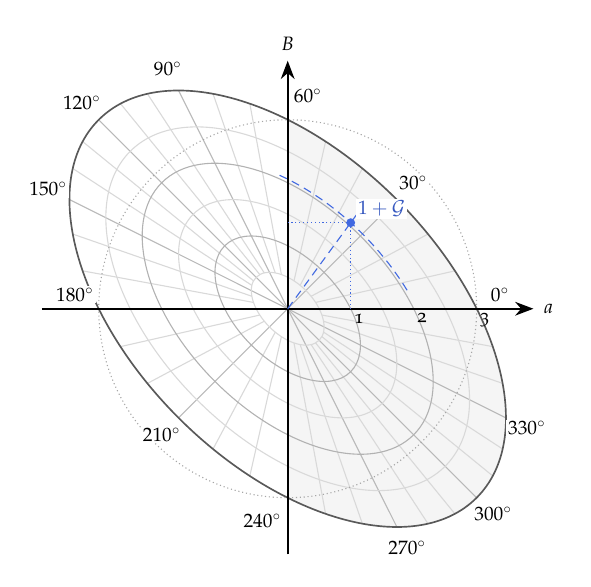
\begin{tikzpicture}[>=Stealth, every node/.style={font=\scriptsize}]
  \begin{scope}\clip (0,-3.121) rectangle (3.121,3.121); \fill[gray!8, rotate=45] (0,0) ellipse ({1.96} and {3.394}); \end{scope}
  \draw[gray!55] (0,0) -- (2.4,0);
  \draw[gray!30] (0.354,0.08) -- (2.123,0.481);
  \draw[gray!30] (0.297,0.158) -- (1.781,0.948);
  \draw[gray!55] (0,0) -- (1.386,1.386);
  \draw[gray!30] (0.158,0.297) -- (0.948,1.781);
  \draw[gray!30] (0.08,0.354) -- (0.481,2.123);
  \draw[gray!55] (0,0) -- (0,2.4);
  \draw[gray!30] (-0.08,0.434) -- (-0.481,2.604);
  \draw[gray!30] (-0.158,0.455) -- (-0.948,2.729);
  \draw[gray!55] (0,0) -- (-1.386,2.771);
  \draw[gray!30] (-0.297,0.455) -- (-1.781,2.729);
  \draw[gray!30] (-0.354,0.434) -- (-2.123,2.604);
  \draw[gray!55] (0,0) -- (-2.4,2.4);
  \draw[gray!30] (-0.434,0.354) -- (-2.604,2.123);
  \draw[gray!30] (-0.455,0.297) -- (-2.729,1.781);
  \draw[gray!55] (0,0) -- (-2.771,1.386);
  \draw[gray!30] (-0.455,0.158) -- (-2.729,0.948);
  \draw[gray!30] (-0.434,0.08) -- (-2.604,0.481);
  \draw[gray!55] (0,0) -- (-2.4,0);
  \draw[gray!30] (-0.354,-0.08) -- (-2.123,-0.481);
  \draw[gray!30] (-0.297,-0.158) -- (-1.781,-0.948);
  \draw[gray!55] (0,0) -- (-1.386,-1.386);
  \draw[gray!30] (-0.158,-0.297) -- (-0.948,-1.781);
  \draw[gray!30] (-0.08,-0.354) -- (-0.481,-2.123);
  \draw[gray!55] (0,0) -- (0,-2.4);
  \draw[gray!30] (0.08,-0.434) -- (0.481,-2.604);
  \draw[gray!30] (0.158,-0.455) -- (0.948,-2.729);
  \draw[gray!55] (0,0) -- (1.386,-2.771);
  \draw[gray!30] (0.297,-0.455) -- (1.781,-2.729);
  \draw[gray!30] (0.354,-0.434) -- (2.123,-2.604);
  \draw[gray!55] (0,0) -- (2.4,-2.4);
  \draw[gray!30] (0.434,-0.354) -- (2.604,-2.123);
  \draw[gray!30] (0.455,-0.297) -- (2.729,-1.781);
  \draw[gray!55] (0,0) -- (2.771,-1.386);
  \draw[gray!30] (0.455,-0.158) -- (2.729,-0.948);
  \draw[gray!30] (0.434,-0.08) -- (2.604,-0.481);
  \draw[gray!30, rotate=45] (0,0) ellipse ({0.327} and {0.566});
  \draw[gray!60, rotate=45] (0,0) ellipse ({0.653} and {1.131});
  \draw[gray!30, rotate=45] (0,0) ellipse ({0.98} and {1.697});
  \draw[gray!60, rotate=45] (0,0) ellipse ({1.306} and {2.263});
  \draw[gray!30, rotate=45] (0,0) ellipse ({1.633} and {2.828});
  \draw[gray!70!black, semithick, rotate=45] (0,0) ellipse ({1.96} and {3.394});
  \draw[gray!70, densely dotted] (0,0) circle (2.4);
  \draw[->, thick] (-3.121,0) -- (3.121,0) node[right] {$a$};
  \draw[->, thick] (0,-3.121) -- (0,3.15) node[above] {$B$};
  \node[fill=white, inner sep=0.6pt, anchor=south] at (2.7,0.06) {$0^\circ$};
  \node[fill=white, inner sep=0.6pt] at (1.598,1.598) {$30^\circ$};
  \node[fill=white, inner sep=0.6pt, anchor=west] at (0.05,2.7) {$60^\circ$};
  \node[fill=white, inner sep=0.6pt] at (-1.52,3.04) {$90^\circ$};
  \node[fill=white, inner sep=0.6pt] at (-2.612,2.612) {$120^\circ$};
  \node[fill=white, inner sep=0.6pt] at (-3.04,1.52) {$150^\circ$};
  \node[fill=white, inner sep=0.6pt, anchor=south] at (-2.7,0.06) {$180^\circ$};
  \node[fill=white, inner sep=0.6pt] at (-1.598,-1.598) {$210^\circ$};
  \node[fill=white, inner sep=0.6pt, anchor=east] at (-0.05,-2.7) {$240^\circ$};
  \node[fill=white, inner sep=0.6pt] at (1.52,-3.04) {$270^\circ$};
  \node[fill=white, inner sep=0.6pt] at (2.612,-2.612) {$300^\circ$};
  \node[fill=white, inner sep=0.6pt] at (3.04,-1.52) {$330^\circ$};
  \node[anchor=north west, inner sep=1pt] at (0.8,-0.02) {1};
  \node[anchor=north west, inner sep=1pt] at (1.6,-0.02) {2};
  \node[anchor=north west, inner sep=1pt] at (2.4,-0.02) {3};
  \draw[RoyalBlue, densely dashed] (1.516,0.235) -- (1.475,0.301) -- (1.432,0.366) -- (1.387,0.431) -- (1.341,0.495) -- (1.294,0.559) -- (1.244,0.622) -- (1.193,0.684) -- (1.141,0.746) -- (1.087,0.806) -- (1.032,0.866) -- (0.976,0.924) -- (0.918,0.982) -- (0.86,1.038) -- (0.8,1.093) -- (0.739,1.146) -- (0.678,1.199) -- (0.615,1.249) -- (0.552,1.299) -- (0.489,1.346) -- (0.424,1.392) -- (0.359,1.436) -- (0.294,1.479) -- (0.228,1.52) -- (0.162,1.559) -- (0.096,1.596) -- (0.03,1.631) -- (-0.037,1.664) -- (-0.103,1.695);
  \draw[RoyalBlue, densely dashed] (0,0) -- (0.976,1.333);
  \draw[RoyalBlue, densely dotted] (0.8,1.093) -- (0.8,0);
  \draw[RoyalBlue, densely dotted] (0.8,1.093) -- (0,1.093);
  \fill[RoyalBlue] (0.8,1.093) circle (1.6pt);
  \node[RoyalBlue!85!black, fill=white, inner sep=0.8pt, anchor=south west] at (0.86,1.133) {$1 + \mathcal{G}$};
\end{tikzpicture}

\smallskip
{\small (b) $\pb = \pi/3$\par}
\end{minipage}
\caption{The polar-like frame of two relative planes, drawn in the chart of the parts: the real part $a$ across and $B = b\,\lvert\Gp\rvert$ up (\Cref{def:rings-rays}). Rings: the magnitudes $M = 0.5$ to $3$, numbered on the real axis, where $M = \lvert a\rvert$. Rays: the angle $\alpha$, every $10^\circ$ and labelled every $30^\circ$; the Composer axis is the upright ray $\alpha = \pb$. The shaded half holds the numbers with a positive real part (\Cref{prop:circle}), and the dotted circle is the ring of magnitude $3$ of the complex plane. (a) At $\pb = 79.86^\circ$, the angle of the worked example, the number $z = 1 + \Gp$ is the point where the ring $1.65988$ and the ray $43.49^\circ$ cross (\Cref{sec:example}). (b) At $\pb = \pi/3$, the angle of \Cref{fig:graph-paper}, the number $1 + \mathcal{G}_{\pi/3}$ lies on the ring $2.05719$ and the ray $35.10^\circ$.}
\label{fig:polar-frame}
\end{figure}

\begin{remark}[Reading the frame]\label{rem:frame-readings}
In the chart of a true relative plane:
\begin{enumerate}
  \item the real axis is the ray $\alpha = 0$, and the Composer axis is the ray $\alpha = \pb$, drawn upright: the chart sets the frame $\{1, \Gp\}$ at a right angle;
  \item the rays are not evenly spread: the angles $\alpha$ from $0$ to $\pb$ fill the first right angle of the chart, and those from $\pb$ to $\pi$ fill the second, so for $\pb < \pi/2$ the rays fan out where the two parts have the same sign and crowd together where their signs differ;
  \item on the real axis $M = \lvert a\rvert$ and on the Composer axis $M = \lvert B\rvert$, so the numbers on the real axis also name the rings; the axes of every ring lie on the rays $\alpha = \pb/2$ and $\pb/2 + \pi$, where the two parts are equal, and on the rays $\alpha = \pb/2 \pm \pi/2$, where they are opposite.
\end{enumerate}
These readings follow from the parametric form of \Cref{thm:ellipse}: the ray $\alpha$ runs through the points $M\,(\sin(\pb - \alpha), \sin\alpha)/\sin\pb$, whose slope $B/a = \sin\alpha/\sin(\pb - \alpha)$ is positive exactly for $0 < \alpha < \pb$, equal to $1$ at $\alpha = \pb/2$ and to $-1$ at $\alpha = \pb/2 + \pi/2$, modulo $\pi$.
\end{remark}

\begin{proposition}[Close to the Composer axis]\label{prop:near-axis}
Let $z = a + b\,\Gp$ with $a > 0$, $b \neq 0$ and $\lvert\eta\rvert = \lvert b\rvert\,\lvert\Gp\rvert/a > 1$, so that its Composer part is the longer leg. The angle $\delta$ between $z$ and the Composer axis is
\[
\delta = \arctan\frac{\sin\pb}{\lvert\eta\rvert + \cos\pb} \ \text{ for } b > 0 , \qquad \delta = \arctan\frac{\sin\pb}{\lvert\eta\rvert - \cos\pb} \ \text{ for } b < 0 ,
\]
and $\delta \approx \sin\pb/\lvert\eta\rvert$ radians when $\lvert\eta\rvert$ is large. For $b > 0$, $\delta$ is the projection angle $\phi$.
\end{proposition}

\begin{proof}
For $b > 0$ the angle between $z$ and $\up$ is $\phi = \pb - \alpha$, and \Cref{thm:triangle} gives $\tan\phi = a\sin\pb/(b\,\lvert\Gp\rvert + a\cos\pb)$. For $b < 0$ the same computation with $-\up$, at the angle $\pi - \pb$ from the positive real axis, replaces $\cos\pb$ by $-\cos\pb$.
\end{proof}

A number whose Composer part is much longer than its real part therefore leans away from the Composer axis, towards the positive real axis, by an angle that shrinks like $1/\lvert\eta\rvert$.

%====================================================================
\section{A Worked Example at \texorpdfstring{$79.86^\circ$}{79.86 degrees}}\label{sec:example}
%====================================================================

Take $\pb = 79.86^\circ$, so that $\cos\pb = 0.17605$, $\sin\pb = 0.98438$ and, by the Axiom, $\lvert\Gp\rvert = 1.16043$, and take the number $z = 1 + \Gp$. \Cref{tab:example} works it through; every value was computed from the definitions and checked against the page (\Cref{sec:verify}). A few lines show the leaning frame at work. The conjugate is not $1 - \Gp$ but $1.40860 - \Gp$: its real part moves, by \Cref{prop:parts-conjugate}, to $2\Sh(z) - \Re(z) = 2(1.20430) - 1$. The square has the Composer part $2.40860\,\Gp = 2\Sh(z)\Com(z)$ (\Cref{thm:parts-product}), not $2\Re(z)\Com(z) = 2\,\Gp$. And the skew flip times $z$ is not real: $(1 + \Gp)(1 - \Gp) = 2.34661 - 0.40860\,\Gp$. In the polar-like frame of \Cref{fig:polar-frame}(a), $z$ is the point where the ring of magnitude $1.65988$ and the ray of $43.49^\circ$ cross.

\begin{table}[tb]
\centering
\small
\renewcommand{\arraystretch}{1.2}
\begin{tabular}{@{}l l l@{}}
\toprule
\textbf{quantity} & \textbf{value} & \textbf{by} \\
\midrule
the two angles of the length $1.16043$ & $10.14^\circ$ and $79.86^\circ$ & \Cref{thm:two-roots} \\
$\Gp^2$ & $-1.34661 + 0.40860\,\Gp$ & \Cref{prop:square-rule} \\
$\Gp^3$ & $-0.55022 - 1.17966\,\Gp$ & \Cref{cor:powers} \\
$\Jp$ & $-0.17885 + 0.87542\,\Gp$ & \Cref{def:turning-unit} \\
square roots of $\Gp$ & $\pm(0.70240 + 0.60529\,\Gp)$ & \Cref{cor:sqrt} \\
\midrule
$\Sh(z)$ and $\Ht(z)$ & $1.20430$ and $1.14231$ & \Cref{def:shadow-height} \\
$\lvert z\rvert$, $\lvert z\rvert^2$ & $1.65988$, $2.75521$ & \Cref{thm:triangle} \\
the angles $\alpha$ and $\phi$ & $43.49^\circ$ and $36.37^\circ$ & \Cref{thm:triangle} \\
$\bar{z}$ & $1.40860 - \Gp$ & \Cref{def:conjugate} \\
$z^2$ & $-0.34661 + 2.40860\,\Gp$ & \Cref{prop:product} \\
$z^3$ & $-3.59005 + 3.04614\,\Gp$ & \Cref{thm:de-moivre} \\
$1/z$ & $0.51125 - 0.36295\,\Gp$ & \Cref{thm:division} \\
$\Jp z$ & $-1.35770 + 1.05427\,\Gp$ & \Cref{thm:turning-unit} \\
square roots of $z$ & $\pm(1.11134 + 0.41782\,\Gp)$, at $21.74^\circ$ & \Cref{thm:roots} \\
$(1 + \Gp)(1 - \Gp)$ & $2.34661 - 0.40860\,\Gp$ & \Cref{rem:skew-flip} \\
signed area of $z$ and $2 - \Gp$ & $-3.42693$ & \Cref{prop:signed-area} \\
\midrule
ellipse of magnitude $M$ & semi-axes $0.92212\,M$ and $1.10167\,M$ & \Cref{thm:ellipse} \\
\bottomrule
\end{tabular}
\caption{The number $z = 1 + \Gp$ at $\pb = 79.86^\circ$. All values are computed with $\pb = 79.86^\circ$ exactly, for which $\lvert\Gp\rvert = 1.1604345$, and rounded to five decimals.}
\label{tab:example}
\end{table}

%====================================================================
\section{Verification and Reproducibility}\label{sec:verify}
%====================================================================

Every true relative plane is a copy of $\C$ (\Cref{cor:bridge}), so every law of this paper can be tested by computing the same quantity twice: once with the laws of the leaning frame, and once with the arrows of the page multiplied as complex numbers. We did this with three scripts, which accompany the paper. They need only Python, SymPy \citep{Meurer2017} and mpmath, which SymPy installs; they draw their random numbers from a fixed seed, and each runs in well under a minute.

\subsection{The paper, statement by statement}

The script \texttt{verify\_paper.py} checks this paper itself. It makes $203$ checks of four kinds.
\begin{enumerate}
  \item \emph{Symbolic proofs} ($79$). Each law of the arithmetic is written in the coordinates $a$, $b$, $c$ and $d$, with $\cos\pb$ and $\sin\pb$ as two symbols tied by $\cos^2\pb + \sin^2\pb = 1$ and the length $\lvert\Gp\rvert$ left free; the difference of the two sides is reduced modulo that relation and must vanish. The identities of the General Sinus are expanded into the sines and cosines of single angles and reduced in the same way. These checks hold for every angle and, for the arithmetic, for every positive length of the Composer Unit. They include the facts about generalized complex numbers recalled in \Cref{sec:intro} and the Cauchy--Riemann equations of \Cref{sec:summary}.
  \item \emph{Numerical checks on the page} ($53$). Each law is evaluated with random coefficients in the relative planes of $45$ angles between $0$ and $\pi$, among them angles close to $0$, $3\pi/4$ and $\pi$, each with the Axiom's length; since the arithmetic holds for any length, many laws are also evaluated in $30$ planes with the lengths $0.37$ and $2.6$. In all, $62\,390$ comparisons were made; two computed values $u$ and $v$ agree when $\lvert u - v\rvert \le 10^{-9}\,(1 + \lvert u\rvert + \lvert v\rvert)$, or $10^{-8}$ in place of $10^{-9}$ where an exponential is computed. The products of \Cref{thm:gs-transform,thm:every-n} were checked to $40$ significant digits for every number of factors from $1$ to $24$.
  \item \emph{Negative controls} ($9$). Each habit of \Cref{tab:habits}, copied into a leaning frame, fails in every one of the $44$ leaning planes tested, and holds at $\pb = \pi/2$.
  \item \emph{Printed numbers} ($62$). Every computed number in the Introduction, in \Cref{sec:gnp,sec:arith,sec:turning,sec:magnitude,sec:example}, in \Cref{tab:example} and in \Cref{fig:graph-paper,fig:fan,fig:turning-unit,fig:spiral,fig:magnitude,fig:polar-frame} is recomputed from the definitions with $50$ digits and rounded as printed.
\end{enumerate}
The script also reads the \LaTeX{} source of the paper and confirms that each of its $51$ numbered statements is covered by at least one check. All the checks pass.

\subsection{The laws, tested independently}

Two further scripts were written earlier, for a forthcoming book by the author, and test the laws of \Cref{sec:arith,sec:turning} and of \Cref{app:formulary}; their output cites the numbering of that book. The first, \texttt{test\_general\_number\_laws.py}, evaluates $144$ laws on the page in $85$ relative planes: $684\,167$ evaluations, with a largest error of $9.5 \times 10^{-13}$ for the exact laws. It also checks $22$ laws exactly, in rational arithmetic on $6\,600$ cases, catches each of $14$ wrong laws given to it as negative controls, and finds each of $5$ errors planted on purpose. The second, \texttt{verify\_general\_number\_algebra.py}, makes $253$ checks: $180$ of them symbolic, for every angle and every length, and the others numerical, among them the printed numbers of the book's worked examples. All $144$ laws hold, and all $253$ checks pass.

%====================================================================
\section{Summary and Outlook}\label{sec:summary}
%====================================================================

\subsection{Summary}

The right angle between the axes of the number plane can be given up. Letting the second axis lean at an angle $\pb$, with a unit whose length $\lvert\cos\pb + \sin\pb\rvert$ is fixed by one axiom, produces a family of relative planes in which the complex plane is the member $\pb = \pi/2$. In every true relative plane the familiar operations survive: sums and products close the plane, every number but zero has an inverse, and the plane is a field. What changes is how the laws read. The square of the Composer Unit is not $-1$ but $2\lvert\Gp\rvert\cos\pb\,\Gp - \lvert\Gp\rvert^2$. The real part of a product, $a_1a_2 - \lvert\Gp\rvert^2b_1b_2$, depends on the angle only through the length $\lvert\Gp\rvert$. The conjugate keeps the mirror image but moves the real part to $a + 2b\lvert\Gp\rvert\cos\pb$, while the skew flip $a - b\,\Gp$ keeps the real part but not the length. And the Composer part of a product is built from the shadows of the factors, $\Com(z_1z_2) = \Sh(z_1)\Com(z_2) + \Sh(z_2)\Com(z_1)$.

The General Sinus is the trigonometry native to these frames. Write $C_\theta = \cos(\theta, \pb - \theta)$ and $S_\theta = \sin(\theta, \pb - \theta)$. Every number but zero is $z = \lvert z\rvert\,(C_\alpha + S_\alpha\,\up)$, with $\alpha$ the angle of its arrow; multiplying multiplies the magnitudes and adds the angles; Euler's formula reads $e^{\theta\Jp} = C_\theta + S_\theta\,\up$; and De Moivre's formula and the $n$ roots of every number but zero follow. The powers of a number carry two trigonometries at once, the General Sinus in their parts and the classical sine and cosine in their shadow and height. Drawn with its parts at right angles, the circle of one magnitude becomes an ellipse whose axes lie on the diagonals, in the ratio $\tan(\pb/2)$. On the side of the trigonometry itself, the product formulas of the General Sinus Transform hold for every number of factors.

\subsection{What is not claimed}

We do not claim a number field beyond the complex numbers, nor a new algebra. Each true relative plane has the points of the complex plane, its algebra is that of the elliptic generalized complex numbers, and the Turning Unit gives an explicit isomorphism with $\C$, so that every result of this paper can be checked against complex arithmetic; \Cref{sec:verify} does exactly that. The contribution is the frame: a family of oblique frames of the number plane, unified by one axiom and read by one trigonometry, together with the complete arithmetic written in it and the exact list of complex habits that fail when the frame leans. Two angles are excluded from the true planes. At $\pb = 0$ the Composer axis falls on the real axis and the plane collapses to a line, and at $\pb = 3\pi/4$ the Composer Unit has length zero.

\subsection{Open questions}

\begin{enumerate}
  \item \emph{Analysis in a leaning frame.} If $f$ is holomorphic, then $f(a + b\,\Gp)$ satisfies $\partial f/\partial b = \Gp\,\partial f/\partial a$, and with $f = U + V\,\Gp$ the Rule of the Square gives the Cauchy--Riemann equations of a leaning frame,
  \[
  \frac{\partial U}{\partial b} = -\lvert\Gp\rvert^2\,\frac{\partial V}{\partial a} , \qquad \frac{\partial V}{\partial b} = \frac{\partial U}{\partial a} + 2\lvert\Gp\rvert\cos\pb\,\frac{\partial V}{\partial a} ,
  \]
  which become the classical equations at $\pb = \pi/2$. Function theory in elliptic complex numbers has been developed, up to a Cauchy--Pompeiu integral formula \citep{AlayonSolarzVanegas2010}. Whether its results, and the derivatives and primitives of the General Sinus \citep[Section~5]{Derraz2026GSP}, take a natural form in the leaning frame remains open.
  \item \emph{Other planes.} The Axiom produces planes of the elliptic kind, isomorphic to $\C$. Leaning frames for the dual and the split-complex numbers, whose geometries are described in \citep{Yaglom1968,HarkinHarkin2004}, and the trigonometries native to them, are a natural next step.
  \item \emph{The length of the unit.} The arithmetic of \Cref{sec:arith,sec:turning,sec:magnitude} holds for any positive length of the Composer Unit; the Axiom enters only through $\lvert\Gp\rvert$. The Axiom's choice, the sum of the two shadows of the direction, has a clear geometric meaning, and a principle that singles it out among all lengths would strengthen the foundations.
  \item \emph{Computation.} The General Sinus Transform replaces the series of the classical functions by products. Its rate of convergence and its error, above all near $\alpha + \phi = \pi$, deserve a complete analysis.
  \item \emph{Applications.} In the forthcoming book the Composer Unit carries the factor $\sqrt{K/G_{\mathrm{N}}}$ between charge and mass, and the angle $79.86^\circ$ is used throughout. Whether a measurement could single out the angle itself, rather than the units in which the constants are written, is an open question there.
\end{enumerate}

Wessel showed that to multiply is to turn. The General Sinus shows that the turning can be read from any angle. Together they leave the number plane as it was, and set free the frame in which we read it.


%====================================================================
\appendix
\section{A Formulary}\label{app:formulary}
%====================================================================

This appendix lists the laws of \Cref{sec:gnp,sec:arith,sec:turning,sec:magnitude}, each beside its complex case.
\begin{itemize}[leftmargin=*]
  \item $z = a + b\,\Gp$ and $w = c + d\,\Gp$ are General Numbers of one true relative plane $\GNp$.
  \item $\lvert\Gp\rvert = \lvert\cos\pb + \sin\pb\rvert$ is the length of the Composer Unit, $\up = \Gp/\lvert\Gp\rvert$ its direction, and $\Jp$ the Turning Unit.
  \item $\theta$ is the angle of a number, its studied angle, and $\pb - \theta$ its projection angle; for short, $C_\theta = \cos(\theta, \pb - \theta)$ and $S_\theta = \sin(\theta, \pb - \theta)$.
\end{itemize}
The right-hand column gives the same law at $\pb = \pi/2$. There $\lvert\Gp\rvert = 1$, the three numbers $\Gp$, $\up$ and $\Jp$ are all $i$, and $C_\theta$ and $S_\theta$ are $\cos\theta$ and $\sin\theta$ (\Cref{cor:gs-classical}). The column writes $\operatorname{Re}$ and $\operatorname{Im}$ for the parts of a complex number, and $r$ for $\lvert z\rvert$ in the polar forms. A few laws are not stated in the body of the paper; a line under each table says where they come from. Every row was checked by the script of \Cref{sec:verify}.

\subsection{The two units}\label{app:units}

\begin{gnlaws}
\gnlaw{the Rule of the Square (\Cref{prop:square-rule})}
  {$\Gp^2 = 2\lvert\Gp\rvert\cos\pb\;\Gp - \lvert\Gp\rvert^2$, \quad $\up^2 = 2\cos\pb\;\up - 1$}
  {$i^2 = -1$}
\gnlaw{the Composer Unit and its conjugate (\Cref{thm:conjugate})}
  {$\Gp + \overline{\Gp} = 2\lvert\Gp\rvert\cos\pb$, \quad $\Gp\,\overline{\Gp} = \lvert\Gp\rvert^2$}
  {$i + (-i) = 0$, \quad $i\,(-i) = 1$}
\gnlaw{the Turning Unit (\Cref{def:turning-unit,thm:turning-unit})}
  {$\Jp = \dfrac{\up - \cos\pb}{\sin\pb} = -\cot\pb + \dfrac{\Gp}{\lvert\Gp\rvert\sin\pb}$, \quad $\Jp^2 = -1$}
  {$i^2 = -1$}
\gnlaw{the square roots of $-1$ (\Cref{thm:turning-unit})}
  {$\Jp$ and $-\Jp$}
  {$i$ and $-i$}
\gnlaw{shadow and height (\Cref{def:shadow-height})}
  {$\Sh(z) = a + b\lvert\Gp\rvert\cos\pb$, \quad $\Ht(z) = b\lvert\Gp\rvert\sin\pb$}
  {$a$ and $b$, the real and imaginary parts}
\gnlaw{the two frames (\Cref{prop:shadow-height})}
  {$z = a + b\,\Gp = \Sh(z) + \Ht(z)\,\Jp$}
  {$z = a + bi$}
\gnlaw{back to the leaning frame (\Cref{prop:shadow-height})}
  {$a = \Sh(z) - \Ht(z)\cot\pb$, \quad $b = \dfrac{\Ht(z)}{\lvert\Gp\rvert\sin\pb}$}
  {$a$ and $b$}
\gnlaw{from the complex plane (\Cref{cor:bridge})}
  {$x + iy = (x - y\cot\pb) + \dfrac{y}{\lvert\Gp\rvert\sin\pb}\,\Gp$}
  {$x + iy$}
\gnlaw{to another true relative plane $\mathbb{G}_{\bar{\psi}}$}
  {$z = a' + b'\,\mathcal{G}_{\bar{\psi}}$ with $b' = \dfrac{\Ht(z)}{\lvert\mathcal{G}_{\bar{\psi}}\rvert\sin\bar{\psi}}$, \quad $a' = \Sh(z) - \Ht(z)\cot\bar{\psi}$}
  {at $\bar{\psi} = \pi/2$: \newline $a' = \Sh(z)$, \quad $b' = \Ht(z)$}
\end{gnlaws}
The shadow and the height are read on the page, so they do not depend on the frame: a number keeps them when it is written in the complex plane or in another relative plane, and the last two rows follow from \Cref{prop:shadow-height}.

\subsection{Arithmetic}\label{app:arithmetic}

\begin{gnlaws}
\gnlaw{sum (\Cref{def:relative-plane})}
  {$(a + b\,\Gp) + (c + d\,\Gp) = (a + c) + (b + d)\,\Gp$}
  {$(a + c) + (b + d)\,i$}
\gnlaw{product (\Cref{prop:product})}
  {$(a + b\,\Gp)(c + d\,\Gp)$ \newline $\quad = (ac - \lvert\Gp\rvert^2bd) + (ad + bc + 2\lvert\Gp\rvert\cos\pb\;bd)\,\Gp$}
  {$(ac - bd) + (ad + bc)\,i$}
\gnlaw{the rules of arithmetic (\Cref{thm:field})}
  {commutativity, associativity, distributivity; $0$, $1$, opposites and inverses: a field}
  {the same}
\gnlaw{conjugate (\Cref{def:conjugate,thm:conjugate})}
  {$\bar{z} = (a + 2b\lvert\Gp\rvert\cos\pb) - b\,\Gp$, the mirror image in the real axis}
  {$\bar{z} = a - bi$}
\gnlaw{the parts of the conjugate (\Cref{prop:parts-conjugate})}
  {$\Re(\bar{z}) = a + 2b\lvert\Gp\rvert\cos\pb$, \quad $\Com(\bar{z}) = -b\,\Gp = -\Com(z)$}
  {$\operatorname{Re}\bar{z} = \operatorname{Re} z$, \newline $\operatorname{Im}\bar{z} = -\operatorname{Im} z$}
\gnlaw{a number times its conjugate (\Cref{thm:conjugate})}
  {$z\bar{z} = a^2 + 2ab\lvert\Gp\rvert\cos\pb + b^2\lvert\Gp\rvert^2 = \lvert z\rvert^2$}
  {$z\bar{z} = a^2 + b^2$}
\gnlaw{a number plus or minus its conjugate (\Cref{thm:conjugate,prop:shadow-height})}
  {$z + \bar{z} = 2\Sh(z)$, \quad $z - \bar{z} = 2\Ht(z)\,\Jp$}
  {$z + \bar{z} = 2a$, \quad $z - \bar{z} = 2bi$}
\gnlaw{the conjugate of a sum and of a product (\Cref{thm:conjugate})}
  {$\overline{z + w} = \bar{z} + \bar{w}$, \quad $\overline{zw} = \bar{z}\,\bar{w}$, \quad $\bar{\bar{z}} = z$}
  {the same}
\gnlaw{inverse (\Cref{thm:division})}
  {$\dfrac{1}{z} = \dfrac{(a + 2b\lvert\Gp\rvert\cos\pb) - b\,\Gp}{a^2 + 2ab\lvert\Gp\rvert\cos\pb + b^2\lvert\Gp\rvert^2}$, \quad $\dfrac{1}{\Gp} = \dfrac{2\lvert\Gp\rvert\cos\pb - \Gp}{\lvert\Gp\rvert^2}$}
  {$\dfrac{1}{z} = \dfrac{a - bi}{a^2 + b^2}$, \quad $\dfrac{1}{i} = -i$}
\gnlaw{quotient (\Cref{thm:division})}
  {$\dfrac{a + b\,\Gp}{c + d\,\Gp} = \dfrac{(ac + 2ad\lvert\Gp\rvert\cos\pb + bd\lvert\Gp\rvert^2) + (bc - ad)\,\Gp}{c^2 + 2cd\lvert\Gp\rvert\cos\pb + d^2\lvert\Gp\rvert^2}$}
  {$\dfrac{(ac + bd) + (bc - ad)\,i}{c^2 + d^2}$}
\gnlaw{the skew flip, which is not the conjugate (\Cref{rem:skew-flip})}
  {$(a + b\,\Gp)(a - b\,\Gp) = a^2 + b^2\lvert\Gp\rvert^2 - 2b^2\lvert\Gp\rvert\cos\pb\;\Gp$, \newline $\lvert a - b\,\Gp\rvert^2 = \lvert z\rvert^2 - 4ab\lvert\Gp\rvert\cos\pb$}
  {$(a + bi)(a - bi) = a^2 + b^2$, \newline $\lvert a - bi\rvert = \lvert z\rvert$}
\end{gnlaws}

\subsection{The plane}\label{app:plane}

\begin{gnlaws}
\gnlaw{magnitude (\Cref{thm:triangle,prop:shadow-height})}
  {$\lvert z\rvert = \sqrt{a^2 + 2ab\lvert\Gp\rvert\cos\pb + b^2\lvert\Gp\rvert^2} = \sqrt{\Sh(z)^2 + \Ht(z)^2}$}
  {$\lvert z\rvert = \sqrt{a^2 + b^2}$}
\gnlaw{the magnitude of a product (\Cref{thm:division})}
  {$\lvert zw\rvert = \lvert z\rvert\,\lvert w\rvert$}
  {the same}
\gnlaw{the two-squares identity, with $zw = s + t\,\Gp$ (\Cref{thm:division})}
  {$(a^2 + 2ab\lvert\Gp\rvert\cos\pb + b^2\lvert\Gp\rvert^2) \times {}$ \newline $(c^2 + 2cd\lvert\Gp\rvert\cos\pb + d^2\lvert\Gp\rvert^2) = {}$ \newline $s^2 + 2st\lvert\Gp\rvert\cos\pb + t^2\lvert\Gp\rvert^2$}
  {$(a^2 + b^2)(c^2 + d^2) = {}$ \newline $(ac - bd)^2 + (ad + bc)^2$}
\gnlaw{angle (\Cref{thm:triangle})}
  {$\tan\theta = \dfrac{\Ht(z)}{\Sh(z)} = \dfrac{b\lvert\Gp\rvert\sin\pb}{a + b\lvert\Gp\rvert\cos\pb}$}
  {$\tan\theta = \dfrac{b}{a}$}
\gnlaw{polar form (\Cref{thm:triangle})}
  {$z = \lvert z\rvert\,\bigl[\cos(\theta, \pb - \theta) + \sin(\theta, \pb - \theta)\,\up\bigr] = \lvert z\rvert\,(C_\theta + S_\theta\,\up)$}
  {$z = r(\cos\theta + i\sin\theta)$}
\gnlaw{the parts in polar form (\Cref{thm:triangle})}
  {$a = \lvert z\rvert\,C_\theta$, \quad $b\,\lvert\Gp\rvert = \lvert z\rvert\,S_\theta$}
  {$a = r\cos\theta$, \quad $b = r\sin\theta$}
\gnlaw{the general Pythagoras identity (\Cref{prop:gs-pythagoras})}
  {$C_\theta^2 + 2\cos\pb\;C_\theta S_\theta + S_\theta^2 = 1$}
  {$\cos^2\theta + \sin^2\theta = 1$}
\gnlaw{the opposite angle}
  {$C_{-\theta} = C_\theta + 2\cos\pb\;S_\theta$, \quad $S_{-\theta} = -S_\theta$}
  {$\cos(-\theta) = \cos\theta$, \newline $\sin(-\theta) = -\sin\theta$}
\gnlaw{the conjugate in polar form (\Cref{thm:euler})}
  {$\bar{z} = \lvert z\rvert\,(C_{-\theta} + S_{-\theta}\,\up)$: the same magnitude, the opposite angle}
  {$\bar{z} = r(\cos\theta - i\sin\theta)$}
\gnlaw{the mirror in the bisector of the two axes}
  {$z \mapsto \up\,\bar{z}$ sends $x + y\,\up$ to $y + x\,\up$}
  {$z \mapsto i\bar{z}$ sends $a + bi$ to $b + ai$}
\gnlaw{reciprocity (\Cref{prop:gs-basic})}
  {$C_{\pb - \theta} = S_\theta$ and $S_{\pb - \theta} = C_\theta$: the unit number at the angle $\pb - \theta$ has the two parts of the one at $\theta$, swapped}
  {$\cos(\tfrac{\pi}{2} - \theta) = \sin\theta$, \newline $\sin(\tfrac{\pi}{2} - \theta) = \cos\theta$}
\end{gnlaws}
The angle is the one of \Cref{thm:triangle}(3), whose ratio $\eta = \lvert\Gp\rvert\,b/a$ gives $\eta\sin\pb/(1 + \eta\cos\pb) = \Ht(z)/\Sh(z)$. The opposite angle follows from $\sin(\pb + \theta) = \sin(\pb - \theta) + 2\cos\pb\sin\theta$. The mirror in the line at the angle $\pb/2$, which halves the angle between the two axes, keeps the length of a number and turns its angle $\theta$ into $\pb - \theta$; reciprocity, $\sin(\alpha, \phi) = \cos(\phi, \alpha)$, says the same in the General Sinus.

\subsection{Multiplying means turning}\label{app:turning}

\begin{gnlaws}
\gnlaw{product in polar form (\Cref{thm:turning})}
  {$\lvert z\rvert\,(C_{\theta_1} + S_{\theta_1}\up) \cdot \lvert w\rvert\,(C_{\theta_2} + S_{\theta_2}\up) = \lvert z\rvert\,\lvert w\rvert\,(C_{\theta_1 + \theta_2} + S_{\theta_1 + \theta_2}\up)$}
  {$r_1r_2\bigl(\cos(\theta_1 + \theta_2) + i\sin(\theta_1 + \theta_2)\bigr)$}
\gnlaw{quotient in polar form (\Cref{thm:turning})}
  {$\dfrac{z}{w} = \dfrac{\lvert z\rvert}{\lvert w\rvert}\,(C_{\theta_1 - \theta_2} + S_{\theta_1 - \theta_2}\up)$}
  {$\dfrac{r_1}{r_2}\bigl(\cos(\theta_1 - \theta_2) + i\sin(\theta_1 - \theta_2)\bigr)$}
\gnlaw{addition along the Composer axis, cosine (\Cref{thm:turning})}
  {$C_{\alpha + \beta} = C_\alpha C_\beta - S_\alpha S_\beta$}
  {$\cos(\alpha + \beta) = {}$ \newline $\cos\alpha\cos\beta - \sin\alpha\sin\beta$}
\gnlaw{addition along the Composer axis, sine (\Cref{thm:turning})}
  {$S_{\alpha + \beta} = C_\alpha S_\beta + S_\alpha C_\beta + 2\cos\pb\;S_\alpha S_\beta$}
  {$\sin(\alpha + \beta) = {}$ \newline $\sin\alpha\cos\beta + \cos\alpha\sin\beta$}
\gnlaw{subtraction, cosine}
  {$C_{\alpha - \beta} = C_\alpha C_\beta + S_\alpha S_\beta + 2\cos\pb\;C_\alpha S_\beta$}
  {$\cos(\alpha - \beta) = {}$ \newline $\cos\alpha\cos\beta + \sin\alpha\sin\beta$}
\gnlaw{subtraction, sine}
  {$S_{\alpha - \beta} = S_\alpha C_\beta - C_\alpha S_\beta$}
  {$\sin(\alpha - \beta) = {}$ \newline $\sin\alpha\cos\beta - \cos\alpha\sin\beta$}
\gnlaw{double angle}
  {$C_{2\alpha} = C_\alpha^2 - S_\alpha^2$, \quad $S_{2\alpha} = 2S_\alpha\,(C_\alpha + \cos\pb\;S_\alpha)$}
  {$\cos 2\alpha = \cos^2\alpha - \sin^2\alpha$, \newline $\sin 2\alpha = 2\sin\alpha\cos\alpha$}
\gnlaw{a turn by $\pb$, the product by $\up$}
  {$C_{\theta + \pb} = -S_\theta$, \quad $S_{\theta + \pb} = C_\theta + 2\cos\pb\;S_\theta$}
  {$\cos(\theta + \tfrac{\pi}{2}) = -\sin\theta$, \newline $\sin(\theta + \tfrac{\pi}{2}) = \cos\theta$}
\gnlaw{a quarter turn, the product by $\Jp$}
  {$C_{\theta + \pi/2} = -C_\theta\cot\pb - \dfrac{S_\theta}{\sin\pb}$, \quad $S_{\theta + \pi/2} = \dfrac{C_\theta}{\sin\pb} + S_\theta\cot\pb$}
  {$\cos(\theta + \tfrac{\pi}{2}) = -\sin\theta$, \newline $\sin(\theta + \tfrac{\pi}{2}) = \cos\theta$}
\gnlaw{a half turn, the product by $-1$}
  {$C_{\theta + \pi} = -C_\theta$, \quad $S_{\theta + \pi} = -S_\theta$}
  {$\cos(\theta + \pi) = -\cos\theta$, \newline $\sin(\theta + \pi) = -\sin\theta$}
\end{gnlaws}
The subtraction formulas are the addition formulas with the opposite angle of \Cref{app:plane}, and the double angle is $\beta = \alpha$. A turn by $\pb$ is the product by $\up = e^{\pb\Jp}$, a quarter turn the product by $\Jp$, and a half turn the product by $e^{\pi\Jp} = -1$; the last is also the $\pi$-addition identity of \Cref{prop:gs-basic}. In the complex plane the turn by $\pb$ and the quarter turn are one and the same.

\subsection{Euler's formula and De Moivre's formula}\label{app:euler}

\begin{gnlaws}
\gnlaw{Euler's formula (\Cref{thm:euler})}
  {$e^{\theta\Jp} = \cos(\theta, \pb - \theta) + \sin(\theta, \pb - \theta)\,\up = C_\theta + S_\theta\,\up$}
  {$e^{i\theta} = \cos\theta + i\sin\theta$}
\gnlaw{exponential form (\Cref{thm:euler})}
  {$z = \lvert z\rvert\,e^{\theta\Jp}$, \quad $\bar{z} = \lvert z\rvert\,e^{-\theta\Jp}$}
  {$z = re^{i\theta}$, \quad $\bar{z} = re^{-i\theta}$}
\gnlaw{the two units as exponentials (\Cref{thm:euler})}
  {$\Gp = \lvert\Gp\rvert\,e^{\pb\Jp}$, \quad $\Jp = e^{(\pi/2)\Jp}$}
  {$i = e^{i\pi/2}$}
\gnlaw{Euler's identity (\Cref{thm:euler})}
  {$e^{\pi\Jp} + 1 = 0$}
  {$e^{i\pi} + 1 = 0$}
\gnlaw{the rate of turning (\Cref{rem:euler-native})}
  {$\dfrac{d}{d\theta}\,e^{\theta\Jp} = \Jp\,e^{\theta\Jp}$}
  {$\dfrac{d}{d\theta}\,e^{i\theta} = i\,e^{i\theta}$}
\gnlaw{De Moivre's formula (\Cref{thm:de-moivre})}
  {$(C_\theta + S_\theta\,\up)^n = C_{n\theta} + S_{n\theta}\,\up$}
  {$(\cos\theta + i\sin\theta)^n = {}$ \newline $\cos n\theta + i\sin n\theta$}
\gnlaw{the powers of the Composer Unit (\Cref{cor:powers})}
  {$\Gp^n = \lvert\Gp\rvert^n C_{n\pb} + \lvert\Gp\rvert^{n-1}S_{n\pb}\,\Gp$ \newline $\quad = -\lvert\Gp\rvert^n\,\dfrac{\sin\,(n - 1)\pb}{\sin\pb} + \lvert\Gp\rvert^{n-1}\,\dfrac{\sin n\pb}{\sin\pb}\,\Gp$}
  {$i^n = \cos\dfrac{n\pi}{2} + i\sin\dfrac{n\pi}{2}$}
\gnlaw{the step rule (\Cref{cor:powers})}
  {$\Gp^{n+1} = 2\lvert\Gp\rvert\cos\pb\;\Gp^n - \lvert\Gp\rvert^2\,\Gp^{n-1}$}
  {$i^{n+1} = -i^{n-1}$}
\gnlaw{the numbers $\sin n\pb/\sin\pb$, for $n = 1, 2, 3, 4$}
  {$1$, \quad $2\cos\pb$, \quad $4\cos^2\pb - 1$, \quad $8\cos^3\pb - 4\cos\pb$}
  {$1$, \quad $0$, \quad $-1$, \quad $0$}
\gnlaw{the exponential of a General Number (\Cref{cor:two-trig})}
  {$e^z = e^{\Sh(z)}\,\bigl(C_{\Ht(z)} + S_{\Ht(z)}\,\up\bigr)$}
  {$e^{a + bi} = e^a(\cos b + i\sin b)$}
\gnlaw{the logarithm, for $-\pi < \theta \le \pi$}
  {$\ln z = \ln\lvert z\rvert + \theta\Jp = (\ln\lvert z\rvert - \theta\cot\pb) + \dfrac{\theta}{\lvert\Gp\rvert\sin\pb}\,\Gp$}
  {$\ln z = \ln r + i\theta$}
\end{gnlaws}
The numbers $\sin n\pb/\sin\pb$ are the Chebyshev polynomials $U_{n-1}(\cos\pb)$ of the second kind; the step rule makes each one from the two before it. The logarithm follows from $z = \lvert z\rvert\,e^{\theta\Jp}$.

\subsection{Roots}\label{app:roots}

\begin{gnlaws}
\gnlaw{the $n$-th roots of $z$ (\Cref{thm:roots})}
  {$w_k = \lvert z\rvert^{1/n}\,\bigl(C_{\theta_k} + S_{\theta_k}\,\up\bigr)$, \quad $\theta_k = \dfrac{\theta + 2\pi k}{n}$, \quad $k = 0, \dots, n - 1$}
  {$w_k = \lvert z\rvert^{1/n}\,e^{i(\theta + 2\pi k)/n}$}
\gnlaw{the roots of unity (\Cref{thm:roots})}
  {$C_{2\pi k/n} + S_{2\pi k/n}\,\up$}
  {$e^{2\pi ik/n}$}
\gnlaw{the square roots of the Composer Unit (\Cref{cor:sqrt})}
  {$\pm\dfrac{\sqrt{\lvert\Gp\rvert}}{2\cos(\pb/2)}\,(1 + \up)$}
  {$\pm\dfrac{1 + i}{\sqrt{2}}$}
\gnlaw{one step along each axis, squared (\Cref{cor:sqrt})}
  {$(1 + \up)^2 = 4\cos^2(\pb/2)\;\up$}
  {$(1 + i)^2 = 2i$}
\gnlaw{the quadratic equation $v^2 + Pv + Q = 0$}
  {$v = \dfrac{-P \pm \sqrt{P^2 - 4Q}}{2}$, with the square roots of the first row}
  {the same}
\end{gnlaws}
The last row holds in every field in which each number has its two square roots, and the first row gives them.

\subsection{The matrix of a General Number}\label{app:matrix}

\begin{gnlaws}
\gnlaw{the matrix of $z$}
  {$\begin{pmatrix} a & -\lvert\Gp\rvert^2 b \\ b & a + 2b\lvert\Gp\rvert\cos\pb \end{pmatrix}$}
  {$\begin{pmatrix} a & -b \\ b & a \end{pmatrix}$}
\gnlaw{products}
  {the matrix of $zw$ is the product of the matrices of $z$ and $w$}
  {the same}
\gnlaw{determinant and trace}
  {$\det = \lvert z\rvert^2$, \quad trace $= 2\Sh(z)$}
  {$\det = a^2 + b^2$, \quad trace $= 2a$}
\gnlaw{the matrix of the Composer Unit}
  {$\mathbf{G} = \begin{pmatrix} 0 & -\lvert\Gp\rvert^2 \\ 1 & 2\lvert\Gp\rvert\cos\pb \end{pmatrix}$, which obeys the Rule of the Square: $\mathbf{G}^2 = 2\lvert\Gp\rvert\cos\pb\,\mathbf{G} - \lvert\Gp\rvert^2\,\mathbf{I}$}
  {$\mathbf{G} = \begin{pmatrix} 0 & -1 \\ 1 & 0 \end{pmatrix}$, with $\mathbf{G}^2 = -\mathbf{I}$}
\end{gnlaws}
Multiplying by $z$ sends $1$ to $a + b\,\Gp$ and $\Gp$ to $-\lvert\Gp\rvert^2 b + (a + 2b\lvert\Gp\rvert\cos\pb)\,\Gp$, by \Cref{prop:product}; these two pairs of coordinates are the columns of the matrix. Its characteristic polynomial is $x^2 - 2\Sh(z)\,x + \lvert z\rvert^2$, whose roots are $z$ and $\bar{z}$.

\subsection{The parts beside the shadow and the height}\label{app:parts}

A number has two pairs of coordinates: its parts, $\Re(z) = a$ and $\Com(z) = b\,\Gp$, counted in the leaning frame, and its shadow and height, counted in the upright frame. In each row the law for the parts comes first, and under it the same law for the shadow and the height; beside them stands the complex case, where the two pairs are one.

\begin{gnlawswide}
\gnlaw{the two pairs (\Cref{def:parts,def:shadow-height})}
  {$\Re(z) = a$, \quad $\Com(z) = b\,\Gp$; \newline $\Sh(z) = a + b\lvert\Gp\rvert\cos\pb$, \quad $\Ht(z) = b\lvert\Gp\rvert\sin\pb$}
  {$\operatorname{Re} z = a$, \quad $\Com(z) = bi$; \newline the two pairs are one}
\gnlaw{from one pair to the other (\Cref{prop:pairs})}
  {$\Re(z) = \Sh(z) - \Ht(z)\cot\pb$, \quad $\Com(z) = \Ht(z)\,\Gp/(\lvert\Gp\rvert\sin\pb)$; \newline $\Sh(z) = \Re(z) + \Sh\bigl(\Com(z)\bigr)$, \quad $\Ht(z) = \Ht\bigl(\Com(z)\bigr)$}
  {the shadow is the real part, and $\Com(z) = i\operatorname{Im} z$}
\gnlaw{sum and real multiple (\Cref{prop:pairs})}
  {$\Re(z + w) = \Re(z) + \Re(w)$ and $\Re(kz) = k\,\Re(z)$ for every real $k$, and the same for $\Com$, for $\Sh$ and for $\Ht$}
  {the same for $\operatorname{Re}$ \newline and for $\operatorname{Im}$}
\gnlaw{magnitude (\Cref{thm:triangle,prop:shadow-height})}
  {$\lvert z\rvert^2 = \Re(z)^2 + 2\cos\pb\;\Re(z)\,b\lvert\Gp\rvert + b^2\lvert\Gp\rvert^2$; \newline $\lvert z\rvert^2 = \Sh(z)^2 + \Ht(z)^2$}
  {$\lvert z\rvert^2 = a^2 + b^2$}
\gnlaw{from a number and its conjugate (\Cref{prop:pairs})}
  {$\Re(z) = (\Gp\bar{z} - \overline{\Gp}z)/(\Gp - \overline{\Gp})$, \quad $\Com(z) = \Gp\,(z - \bar{z})/(\Gp - \overline{\Gp})$, \newline with $\Gp - \overline{\Gp} = 2\lvert\Gp\rvert\sin\pb\;\Jp$; \newline $\Sh(z) = (z + \bar{z})/2$, \quad $\Ht(z)\,\Jp = (z - \bar{z})/2$}
  {$\operatorname{Re} z = (z + \bar{z})/2$, \newline $i\operatorname{Im} z = (z - \bar{z})/2$}
\gnlaw{real numbers, pure Composer numbers and multiples of $\Jp$ (\Cref{prop:pairs})}
  {$\Com(z) = 0$ exactly when $\bar{z} = z$, \newline $\Re(z) = 0$ exactly when $\Gp\bar{z} = \overline{\Gp}z$; \newline $\Ht(z) = 0$ exactly when $\bar{z} = z$, \newline $\Sh(z) = 0$ exactly when $\bar{z} = -z$}
  {real numbers: $\bar{z} = z$, \newline imaginary numbers: $\bar{z} = -z$}
\gnlaw{product (\Cref{thm:parts-product})}
  {$\Re(zw) = \Re(z)\Re(w) - \lvert\Gp\rvert^2 bd$, \newline $\Com(zw) = \Sh(z)\Com(w) + \Sh(w)\Com(z)$; \newline $\Sh(zw) = \Sh(z)\Sh(w) - \Ht(z)\Ht(w)$, \newline $\Ht(zw) = \Sh(z)\Ht(w) + \Sh(w)\Ht(z)$}
  {$\operatorname{Re}(zw) = ac - bd$, \newline $\operatorname{Im}(zw) = ad + bc$}
\gnlaw{square (\Cref{thm:parts-product})}
  {$\Re(z^2) = \Re(z)^2 - \lvert\Gp\rvert^2 b^2$, \quad $\Com(z^2) = 2\Sh(z)\Com(z)$; \newline $\Sh(z^2) = \Sh(z)^2 - \Ht(z)^2$, \quad $\Ht(z^2) = 2\Sh(z)\Ht(z)$}
  {$\operatorname{Re}(z^2) = a^2 - b^2$, \newline $\operatorname{Im}(z^2) = 2ab$}
\gnlaw{conjugate (\Cref{prop:parts-conjugate})}
  {$\Re(\bar{z}) = 2\Sh(z) - \Re(z)$, \quad $\Com(\bar{z}) = -\Com(z)$, \newline so $\Sh(z) = \bigl[\Re(z) + \Re(\bar{z})\bigr]/2$; \newline $\Sh(\bar{z}) = \Sh(z)$, \quad $\Ht(\bar{z}) = -\Ht(z)$}
  {$\operatorname{Re}\bar{z} = a$, \newline $\operatorname{Im}\bar{z} = -b$}
\gnlaw{inverse (\Cref{prop:parts-conjugate})}
  {$\Re(1/z) = \bigl[2\Sh(z) - \Re(z)\bigr]/\lvert z\rvert^2$, \quad $\Com(1/z) = -\Com(z)/\lvert z\rvert^2$; \newline $\Sh(1/z) = \Sh(z)/\lvert z\rvert^2$, \quad $\Ht(1/z) = -\Ht(z)/\lvert z\rvert^2$}
  {the two parts of \newline $\dfrac{a - bi}{a^2 + b^2}$}
\gnlaw{quotient, with the top $z\bar{w}$ (\Cref{prop:parts-conjugate,prop:signed-area})}
  {$\Re(z/w) = \Re(z\bar{w})/\lvert w\rvert^2$ \ with \ $\Re(z\bar{w}) = \Re(z)\Re(\bar{w}) + \lvert\Gp\rvert^2 bd$, \newline $\Com(z/w) = \Com(z\bar{w})/\lvert w\rvert^2$ \ with \ $\Com(z\bar{w}) = \Sh(w)\Com(z) - \Sh(z)\Com(w)$; \newline $\Sh(z/w) = \Sh(z\bar{w})/\lvert w\rvert^2$ \ with \ $\Sh(z\bar{w}) = \Sh(z)\Sh(w) + \Ht(z)\Ht(w)$, \newline $\Ht(z/w) = \Ht(z\bar{w})/\lvert w\rvert^2$ \ with \ $\Ht(z\bar{w}) = \Sh(w)\Ht(z) - \Sh(z)\Ht(w)$}
  {the two parts of \newline $\dfrac{(ac + bd) + (bc - ad)\,i}{c^2 + d^2}$}
\gnlaw{a quarter turn, the product by $\Jp$ (\Cref{thm:turning-unit,thm:parts-product})}
  {$\Re(\Jp z) = -\Ht(z) - \Sh(z)\cot\pb$, \quad $\Com(\Jp z) = \Sh(z)\,\Gp/(\lvert\Gp\rvert\sin\pb)$; \newline $\Sh(\Jp z) = -\Ht(z)$, \quad $\Ht(\Jp z) = \Sh(z)$}
  {$\operatorname{Re}(iz) = -b$, \newline $\operatorname{Im}(iz) = a$}
\gnlaw{the product by the Composer Unit (\Cref{thm:parts-product})}
  {$\Re(\Gp z) = -\lvert\Gp\rvert^2 b$, \quad $\Com(\Gp z) = \Re(\bar{z})\,\Gp$; \newline $\Sh(\Gp z) = \lvert\Gp\rvert\bigl(\Sh(z)\cos\pb - \Ht(z)\sin\pb\bigr)$, \newline $\Ht(\Gp z) = \lvert\Gp\rvert\bigl(\Sh(z)\sin\pb + \Ht(z)\cos\pb\bigr)$}
  {the product by $i$, \newline as in the row above}
\gnlaw{the powers of the Composer Unit (\Cref{cor:powers,cor:two-trig})}
  {$\Re(\Gp^n) = -\lvert\Gp\rvert^n\sin\,(n - 1)\pb/\sin\pb$, \quad $\Com(\Gp^n) = \lvert\Gp\rvert^{n-1}\,(\sin n\pb/\sin\pb)\,\Gp$; \newline $\Sh(\Gp^n) = \lvert\Gp\rvert^n\cos n\pb$, \quad $\Ht(\Gp^n) = \lvert\Gp\rvert^n\sin n\pb$}
  {$\operatorname{Re}(i^n) = \cos(n\pi/2)$, \newline $\operatorname{Im}(i^n) = \sin(n\pi/2)$}
\gnlaw{powers, and for $n = 1$ the polar form (\Cref{cor:two-trig})}
  {$\Re(z^n) = \lvert z\rvert^n C_{n\theta}$, \quad $\Com(z^n) = \lvert z\rvert^n S_{n\theta}\,\up$; \newline $\Sh(z^n) = \lvert z\rvert^n\cos n\theta$, \quad $\Ht(z^n) = \lvert z\rvert^n\sin n\theta$}
  {$\operatorname{Re}(z^n) = r^n\cos n\theta$, \newline $\operatorname{Im}(z^n) = r^n\sin n\theta$}
\gnlaw{exponential (\Cref{cor:two-trig})}
  {$\Re(e^z) = e^{\Sh(z)}\,C_{\Ht(z)}$, \quad $\Com(e^z) = e^{\Sh(z)}\,S_{\Ht(z)}\,\up$; \newline $\Sh(e^z) = e^{\Sh(z)}\cos\Ht(z)$, \quad $\Ht(e^z) = e^{\Sh(z)}\sin\Ht(z)$}
  {$\operatorname{Re}(e^z) = e^a\cos b$, \newline $\operatorname{Im}(e^z) = e^a\sin b$}
\gnlaw{signed area and dot product (\Cref{prop:signed-area})}
  {$\Com(\bar{z}w) = (ad - bc)\,\Gp$, \quad $\Re(\bar{z}w) = \Re(\bar{z})\Re(w) + \lvert\Gp\rvert^2 bd$; \newline $\Ht(\bar{z}w) = \Sh(z)\Ht(w) - \Ht(z)\Sh(w)$, which is $(ad - bc)\,\lvert\Gp\rvert\sin\pb$, \newline $\Sh(\bar{z}w) = \Sh(z)\Sh(w) + \Ht(z)\Ht(w)$}
  {$\operatorname{Im}(\bar{z}w) = ad - bc$, \newline $\operatorname{Re}(\bar{z}w) = ac + bd$}
\gnlaw{size (\Cref{rem:longer})}
  {$\lvert\Re(z)\rvert \le \lvert z\rvert/\sin\pb$, \quad $\lvert\Com(z)\rvert \le \lvert z\rvert/\sin\pb$; \newline $\lvert\Sh(z)\rvert \le \lvert z\rvert$, \quad $\lvert\Ht(z)\rvert \le \lvert z\rvert$}
  {$\lvert\operatorname{Re} z\rvert \le \lvert z\rvert$, \newline $\lvert\operatorname{Im} z\rvert \le \lvert z\rvert$}
\end{gnlawswide}
From the third row on, the laws for the shadow and the height are the laws of the complex numbers, read in the upright frame, word for word; the first two rows pass from one frame to the other. The laws for the parts are the same arithmetic counted in the leaning frame, where the lean shows. Written out in the coordinates $a$, $b$, $c$ and $d$, two of them stand out: the Composer part of $\bar{z}w$, $(ad - bc)\,\Gp$, has a coordinate that does not depend on the angle at all, and the real part of $zw$, $ac - \lvert\Gp\rvert^2bd$, depends on it only through the length $\lvert\Gp\rvert$. The two rows on the products by $\Jp$ and by $\Gp$ are \Cref{thm:parts-product} with $w = \Jp$ and $w = \Gp$.

\medskip
\noindent\begin{minipage}{\textwidth}
\setlength{\parindent}{0pt}
The parts, the shadow and the height of six numbers that recur:
\begin{center}
\small
\renewcommand{\arraystretch}{1.2}
\begin{tabular}{@{}lllll@{}}
\toprule
 & \textsc{real part} & \textsc{Composer part} & \textsc{shadow} & \textsc{height} \\
\midrule
$1$ & $1$ & $0$ & $1$ & $0$ \\
$\Gp$ & $0$ & $\Gp$ & $\lvert\Gp\rvert\cos\pb$ & $\lvert\Gp\rvert\sin\pb$ \\
$\overline{\Gp}$ & $2\lvert\Gp\rvert\cos\pb$ & $-\Gp$ & $\lvert\Gp\rvert\cos\pb$ & $-\lvert\Gp\rvert\sin\pb$ \\
$\Gp^2$ & $-\lvert\Gp\rvert^2$ & $2\lvert\Gp\rvert\cos\pb\;\Gp$ & $\lvert\Gp\rvert^2\cos 2\pb$ & $\lvert\Gp\rvert^2\sin 2\pb$ \\
$1/\Gp$ & $2\cos\pb/\lvert\Gp\rvert$ & $-\Gp/\lvert\Gp\rvert^2$ & $\cos\pb/\lvert\Gp\rvert$ & $-\sin\pb/\lvert\Gp\rvert$ \\
$\Jp$ & $-\cot\pb$ & $\Gp/(\lvert\Gp\rvert\sin\pb)$ & $0$ & $1$ \\
\bottomrule
\end{tabular}
\end{center}
At $\pb = \pi/2$ the six numbers are $1$, $i$, $-i$, $-1$, $-i$ and $i$. The first two columns then give the real part and $i$ times the imaginary part, and the last two the real part and the imaginary part.
\end{minipage}

% Bibliography embedded (plainnat output of gn-paper.bib), so no BibTeX run is needed.
\begin{thebibliography}{28}
\providecommand{\natexlab}[1]{#1}
\providecommand{\url}[1]{\texttt{#1}}
\expandafter\ifx\csname urlstyle\endcsname\relax
  \providecommand{\doi}[1]{doi: #1}\else
  \providecommand{\doi}{doi: \begingroup \urlstyle{rm}\Url}\fi

\bibitem[Alay{\'o}n-Solarz and Vanegas(2010)]{AlayonSolarzVanegas2010}
Daniel Alay{\'o}n-Solarz and Carmen~Judith Vanegas.
\newblock The {Cauchy--Pompeiu} integral formula in elliptic complex numbers.
\newblock arXiv:1002.3405, 2010.

\bibitem[Argand(1806)]{Argand1806}
Jean-Robert Argand.
\newblock \emph{Essai sur une mani{\`e}re de repr{\'e}senter les quantit{\'e}s
  imaginaires dans les constructions g{\'e}om{\'e}triques}.
\newblock Paris, 1806.

\bibitem[Bombelli(1572)]{Bombelli1572}
Rafael Bombelli.
\newblock \emph{L'Algebra}.
\newblock Giovanni Rossi, Bologna, 1572.

\bibitem[Brooks and Smith(1987)]{BrooksSmith1987}
Alison~S. Brooks and Catherine~C. Smith.
\newblock {Ishango} revisited: New age determinations and cultural
  interpretations.
\newblock \emph{African Archaeological Review}, 5:\penalty0 65--78, 1987.

\bibitem[Cardano(1545)]{Cardano1545}
Gerolamo Cardano.
\newblock \emph{Artis Magnae, sive de Regulis Algebraicis}.
\newblock Johannes Petreius, N{\"u}rnberg, 1545.

\bibitem[Colebrooke(1817)]{Colebrooke1817}
Henry~Thomas Colebrooke.
\newblock \emph{Algebra, with Arithmetic and Mensuration, from the Sanscrit of
  Brahmegupta and Bh{\'a}scara}.
\newblock John Murray, London, 1817.

\bibitem[de~Coulomb(1788)]{Coulomb1785}
Charles-Augustin de~Coulomb.
\newblock Premier m{\'e}moire sur l'{\'e}lectricit{\'e} et le magn{\'e}tisme.
\newblock In \emph{Histoire de l'Acad{\'e}mie Royale des Sciences, Ann{\'e}e
  1785}, pages 569--577. Paris, 1788.

\bibitem[Derraz(2017)]{Derraz2017}
Mostafa Derraz.
\newblock {General Sinus}.
\newblock \emph{International Journal of Swarm Intelligence and Evolutionary
  Computation}, 6\penalty0 (2), 2017.
\newblock \doi{10.4172/2090-4908.1000155}.

\bibitem[Derraz(2026)]{Derraz2026GSP}
Mostafa Derraz.
\newblock {General Sinus Principles: Extension of Trigonometric Functions}.
\newblock \emph{Research Square}, 2026.
\newblock \doi{10.21203/rs.3.rs-9525842/v1}.
\newblock Preprint, posted 4 May 2026.

\bibitem[d'Errico et~al.(2012)d'Errico, Backwell, Villa, Degano, Lucejko,
  Bamford, Higham, Colombini, and Beaumont]{dErrico2012}
Francesco d'Errico, Lucinda Backwell, Paola Villa, Ilaria Degano, Jeannette~J.
  Lucejko, Marion~K. Bamford, Thomas F.~G. Higham, Maria~Perla Colombini, and
  Peter~B. Beaumont.
\newblock Early evidence of {San} material culture represented by organic
  artifacts from {Border Cave}, {South Africa}.
\newblock \emph{Proceedings of the National Academy of Sciences}, 109\penalty0
  (33):\penalty0 13214--13219, 2012.

\bibitem[Descartes(1637)]{Descartes1637}
Ren{\'e} Descartes.
\newblock \emph{La G{\'e}om{\'e}trie}.
\newblock Ian Maire, Leiden, 1637.
\newblock Appendix to the Discours de la M{\'e}thode.

\bibitem[Euler(1748)]{Euler1748}
Leonhard Euler.
\newblock \emph{Introductio in analysin infinitorum}.
\newblock Marcum-Michaelem Bousquet, Lausanne, 1748.

\bibitem[Gauss(1831)]{Gauss1831}
Carl~Friedrich Gauss.
\newblock Theoria residuorum biquadraticorum, commentatio secunda, 1831.
\newblock With the author's announcement in the G{\"o}ttingische gelehrte
  Anzeigen; in Werke, vol.~2, G{\"o}ttingen, 1863.

\bibitem[Gradshteyn and Ryzhik(2015)]{GradshteynRyzhik2015}
I.~S. Gradshteyn and I.~M. Ryzhik.
\newblock \emph{Table of Integrals, Series, and Products}.
\newblock Academic Press, Amsterdam, eighth edition, 2015.
\newblock Edited by D. Zwillinger and V. Moll.

\bibitem[Hamilton(1837)]{Hamilton1837}
William~Rowan Hamilton.
\newblock Theory of conjugate functions, or algebraic couples; with a
  preliminary and elementary essay on algebra as the science of pure time.
\newblock \emph{Transactions of the Royal Irish Academy}, 17:\penalty0
  293--422, 1837.

\bibitem[Hamilton(1844)]{Hamilton1844}
William~Rowan Hamilton.
\newblock On quaternions; or on a new system of imaginaries in algebra.
\newblock \emph{Philosophical Magazine}, 25:\penalty0 489--495, 1844.

\bibitem[Harkin and Harkin(2004)]{HarkinHarkin2004}
Anthony~A. Harkin and Joseph~B. Harkin.
\newblock Geometry of generalized complex numbers.
\newblock \emph{Mathematics Magazine}, 77\penalty0 (2):\penalty0 118--129,
  2004.
\newblock \doi{10.1080/0025570X.2004.11953236}.

\bibitem[Kantor and Solodovnikov(1989)]{KantorSolodovnikov1989}
I.~L. Kantor and A.~S. Solodovnikov.
\newblock \emph{Hypercomplex Numbers: An Elementary Introduction to Algebras}.
\newblock Springer-Verlag, New York, 1989.
\newblock Translated from the Russian by A. Shenitzer.

\bibitem[Kline(1972)]{Kline1972}
Morris Kline.
\newblock \emph{Mathematical Thought from Ancient to Modern Times}.
\newblock Oxford University Press, New York, 1972.

\bibitem[Mason and Handscomb(2003)]{MasonHandscomb2003}
J.~C. Mason and D.~C. Handscomb.
\newblock \emph{{Chebyshev} Polynomials}.
\newblock Chapman \& Hall/CRC, Boca Raton, 2003.

\bibitem[Meurer et~al.(2017)Meurer, Smith, Paprocki, {\v{C}}ert{\'\i}k,
  Kirpichev, Rocklin, Kumar, Ivanov, Moore, Singh, et~al.]{Meurer2017}
Aaron Meurer, Christopher~P. Smith, Mateusz Paprocki, Ond{\v{r}}ej
  {\v{C}}ert{\'\i}k, Sergey~B. Kirpichev, Matthew Rocklin, Amit Kumar, Sergiu
  Ivanov, Jason~K. Moore, Sartaj Singh, et~al.
\newblock {SymPy}: symbolic computing in {Python}.
\newblock \emph{PeerJ Computer Science}, 3:\penalty0 e103, 2017.
\newblock \doi{10.7717/peerj-cs.103}.

\bibitem[Mokhithi and Shock(2020)]{MokhithiShock2020}
M.~Mokhithi and J.~Shock.
\newblock Introduction to complex numbers.
\newblock Lecture notes, version 1, Department of Mathematics and Applied
  Mathematics, University of Cape Town, 2020.
\newblock Licensed under CC BY 4.0.

\bibitem[Newton(1687)]{Newton1687}
Isaac Newton.
\newblock \emph{Philosophi{\ae} Naturalis Principia Mathematica}.
\newblock Joseph Streater, London, 1687.

\bibitem[Plofker(2009)]{Plofker2009}
Kim Plofker.
\newblock \emph{Mathematics in India}.
\newblock Princeton University Press, Princeton, 2009.

\bibitem[Shen et~al.(1999)Shen, Crossley, and Lun]{Shen1999}
Kangshen Shen, John~N. Crossley, and Anthony W.-C. Lun.
\newblock \emph{The Nine Chapters on the Mathematical Art: Companion and
  Commentary}.
\newblock Oxford University Press, Oxford, 1999.

\bibitem[Weil(1984)]{Weil1984}
Andr{\'e} Weil.
\newblock \emph{Number Theory: An Approach through History from {Hammurapi} to
  {Legendre}}.
\newblock Birkh{\"a}user, Boston, 1984.

\bibitem[Wessel(1799)]{Wessel1799}
Caspar Wessel.
\newblock {Om Directionens analytiske Betegning}.
\newblock \emph{Nye Samling af det Kongelige Danske Videnskabernes Selskabs
  Skrifter}, 5:\penalty0 469--518, 1799.
\newblock Presented to the Royal Danish Academy in 1797.

\bibitem[Yaglom(1968)]{Yaglom1968}
I.~M. Yaglom.
\newblock \emph{Complex Numbers in Geometry}.
\newblock Academic Press, New York, 1968.
\newblock Translated from the Russian by E. J. F. Primrose.

\end{thebibliography}

\end{document}
